\begin{figure*}
	\begin{subfigure}[t]{.49\linewidth}
		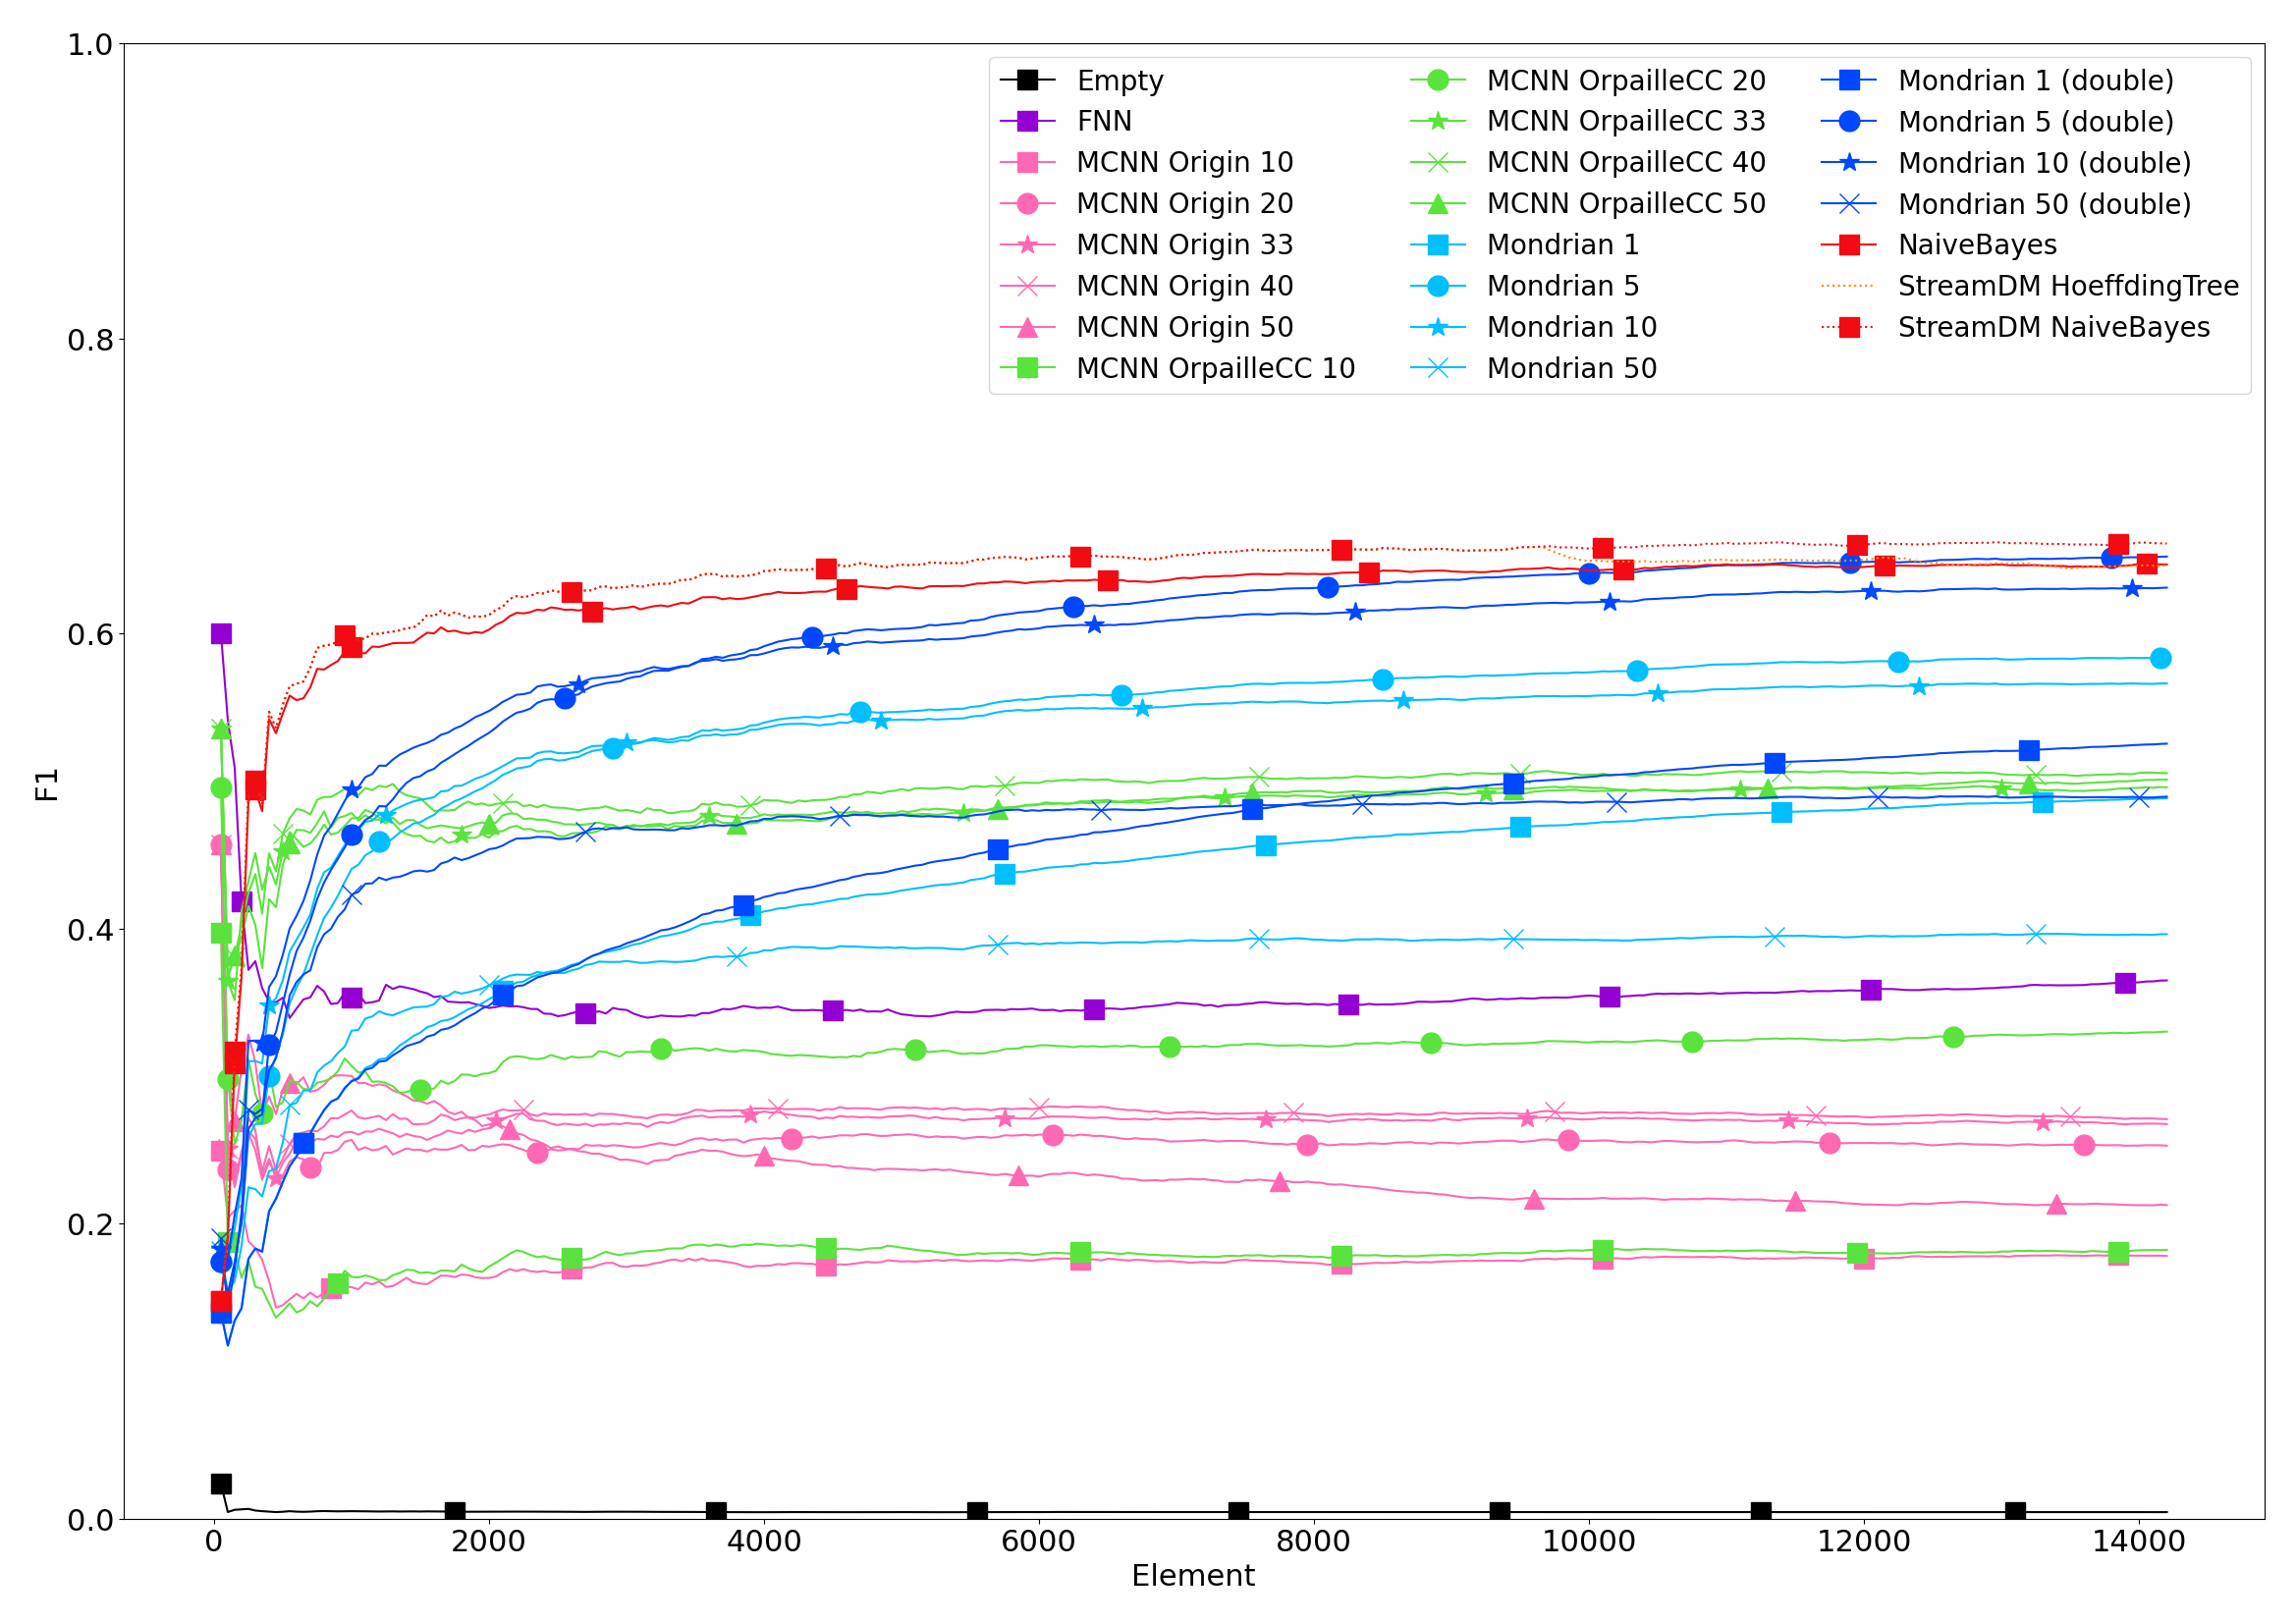
\includegraphics[width=\linewidth]{figures/results/banos_6_f1.png}
		\caption{\banosdataset}
		\label{fig:f1-banos}
	\end{subfigure}
	\hfill
	\begin{subfigure}[t]{.49\linewidth}
		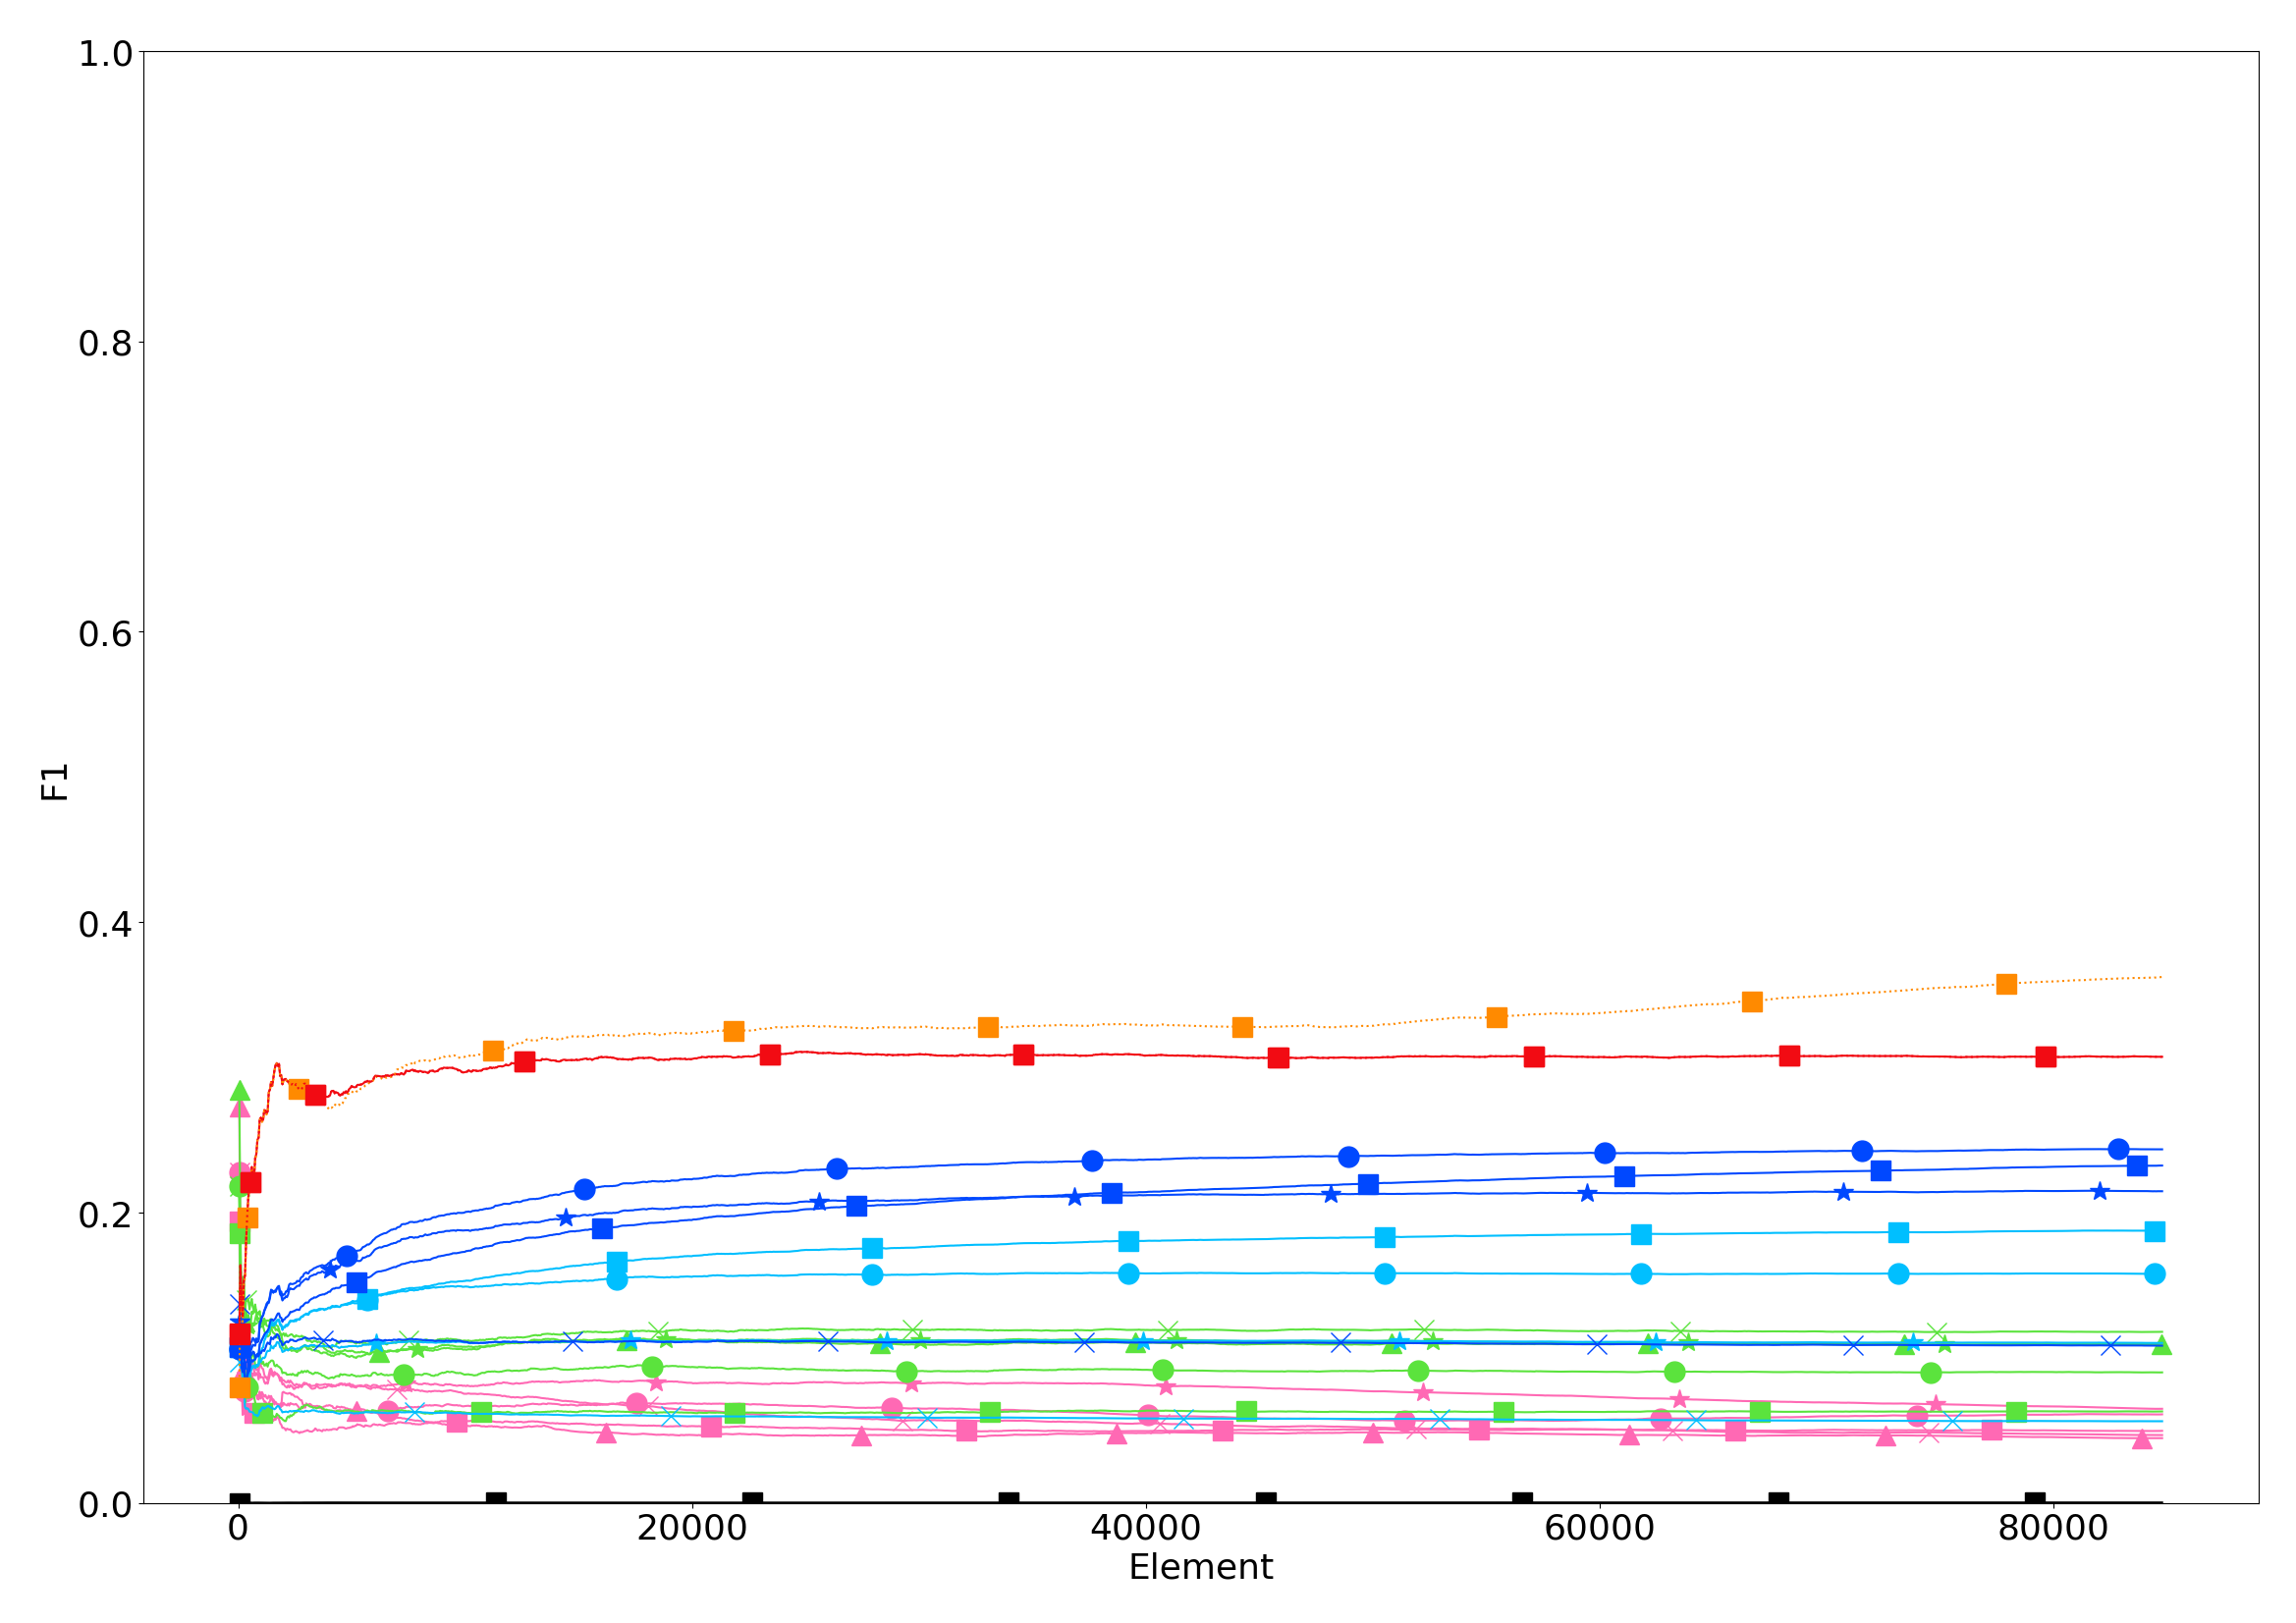
\includegraphics[width=\linewidth]{figures/results/recofit_6_f1.png}
		\caption{\recofitdataset}
		\label{fig:f1-recofit}
	\end{subfigure}\\
	\begin{subfigure}[t]{.49\linewidth}
		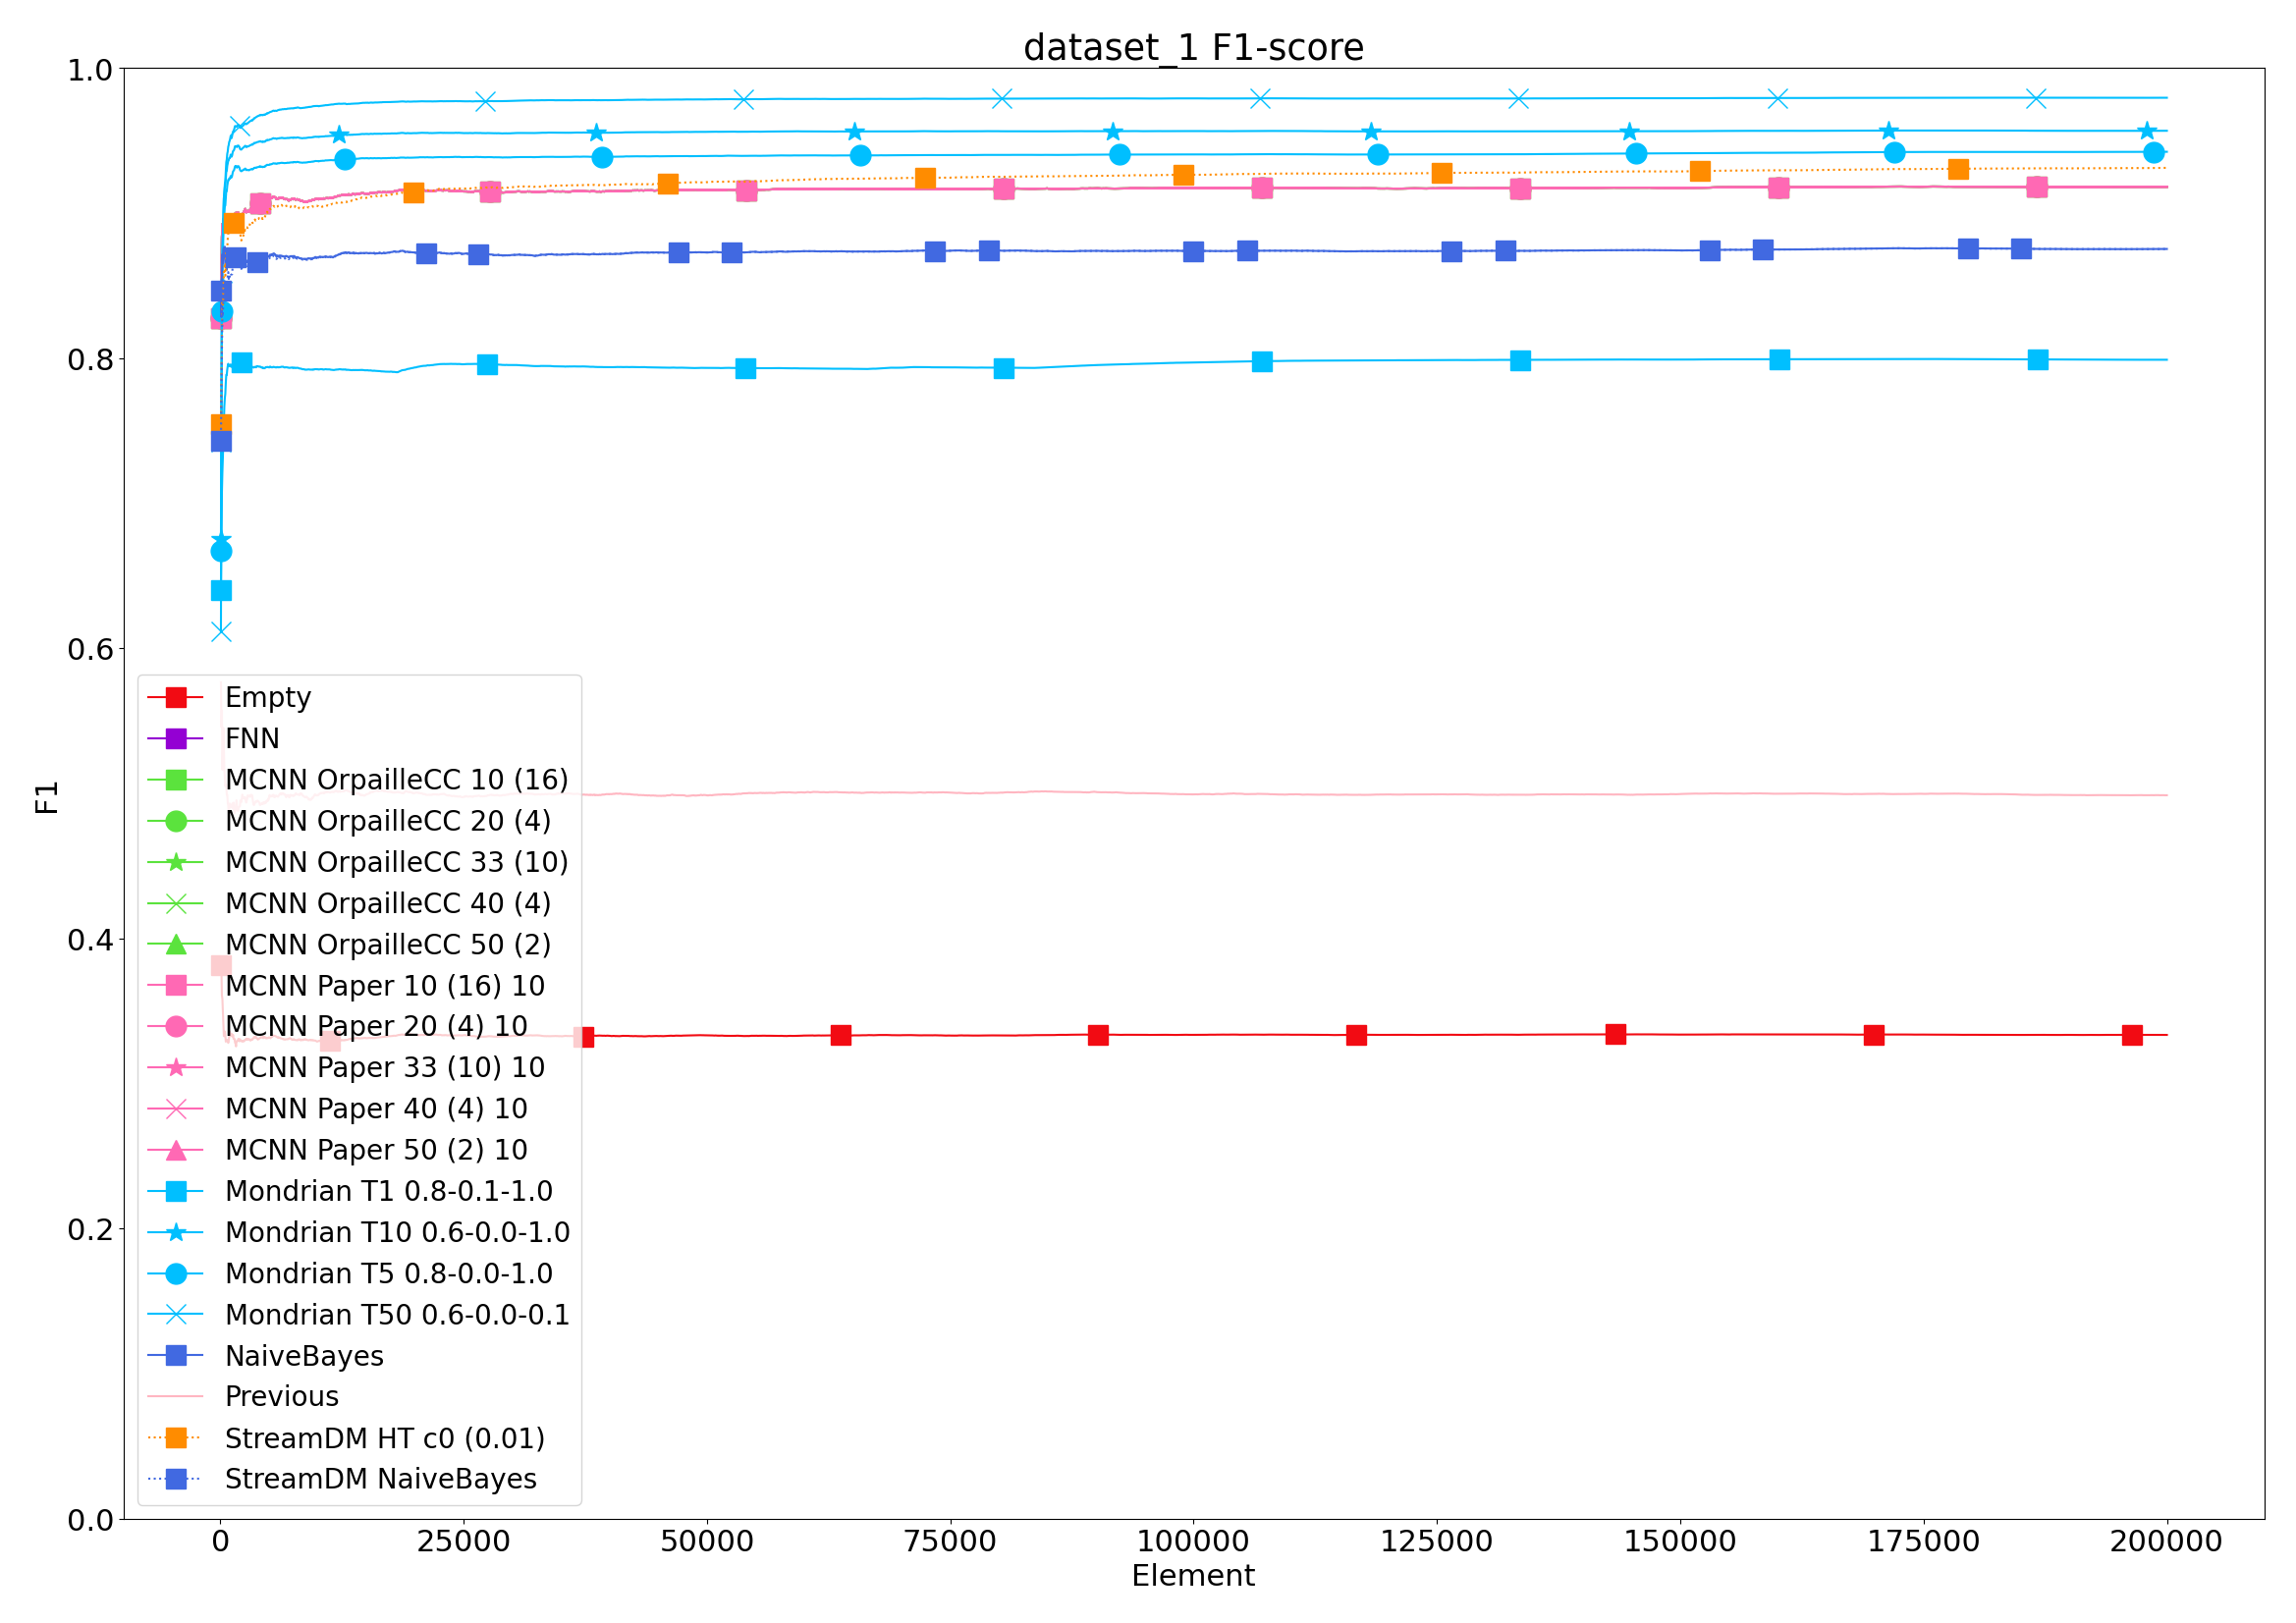
\includegraphics[width=\linewidth]{figures/results/dataset_1_f1.png}
		\caption{Hyperplane (MOA)}
		\label{fig:f1-dataset_1}
	\end{subfigure}
	\hfill
	\begin{subfigure}[t]{.49\linewidth}
		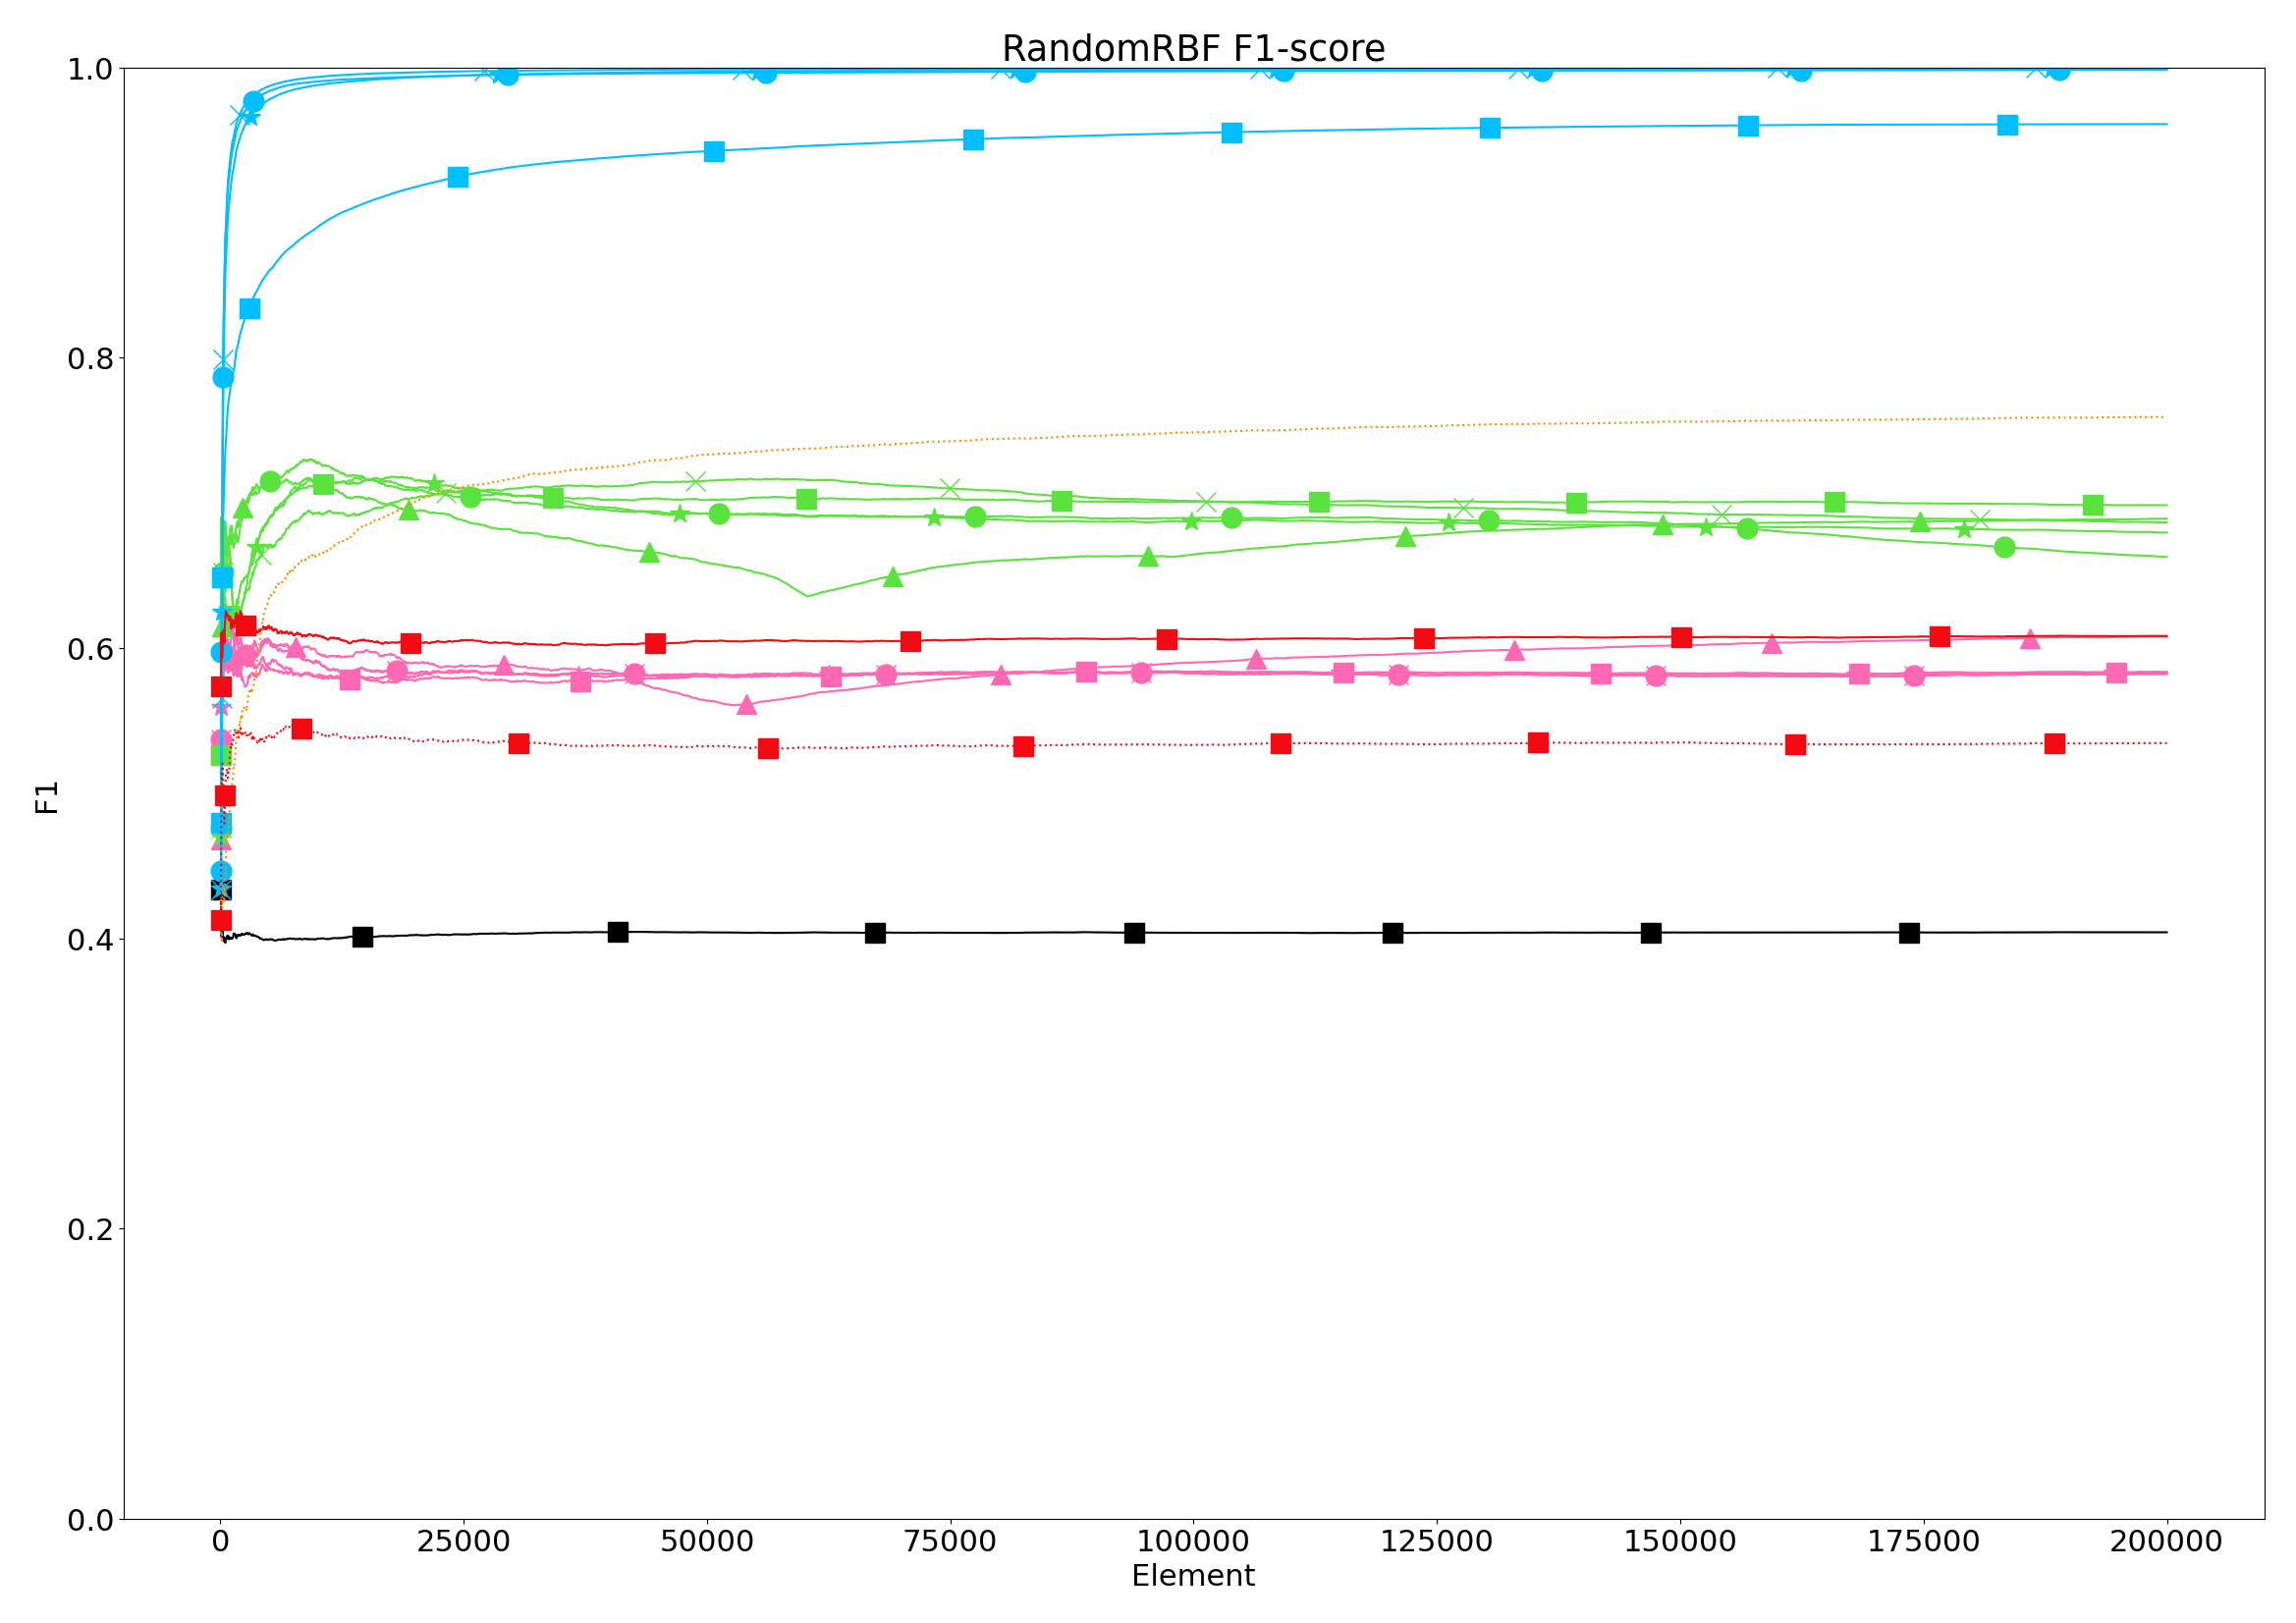
\includegraphics[width=\linewidth]{figures/results/dataset_2_f1.png}
		\caption{RandomRBF (MOA)}
		\label{fig:f1-dataset_2}
	\end{subfigure}\\
	\begin{subfigure}[t]{.49\linewidth}
		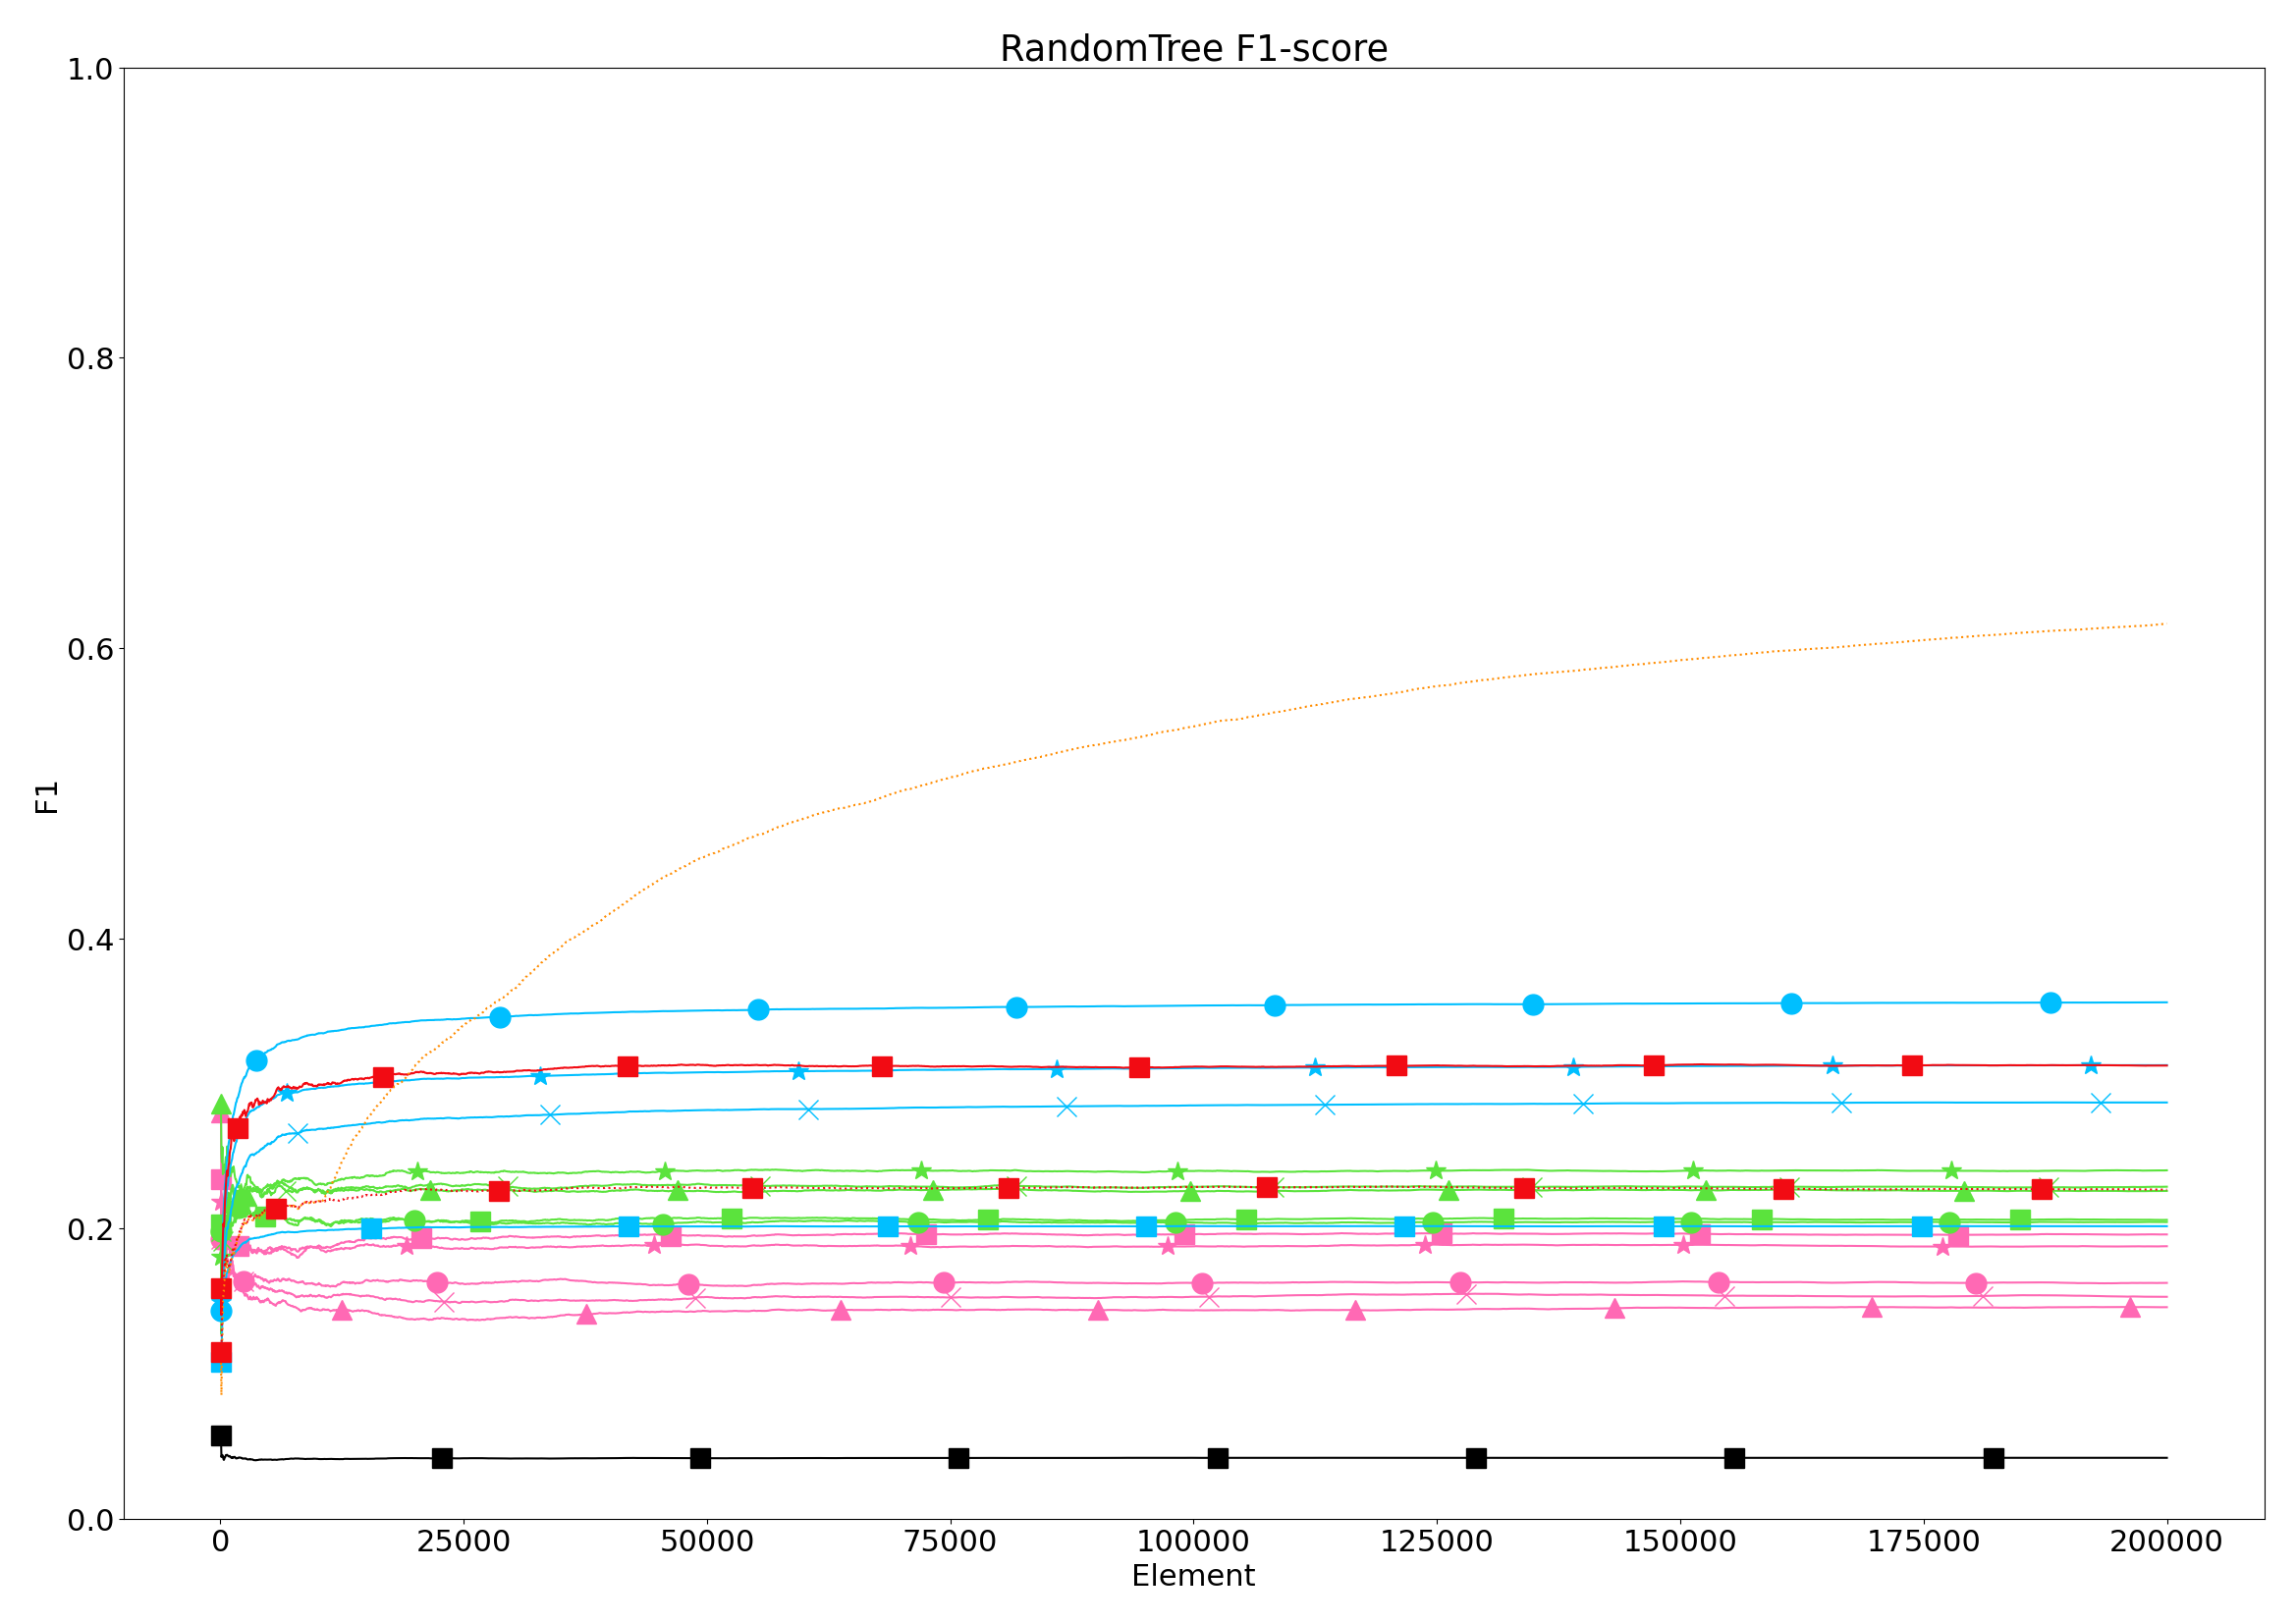
\includegraphics[width=\linewidth]{figures/results/dataset_3_f1.png}
		\caption{RandomTree (MOA)}
		\label{fig:f1-dataset_3}
	\end{subfigure}
	\hfill
	\begin{subfigure}[t]{.49\linewidth}
		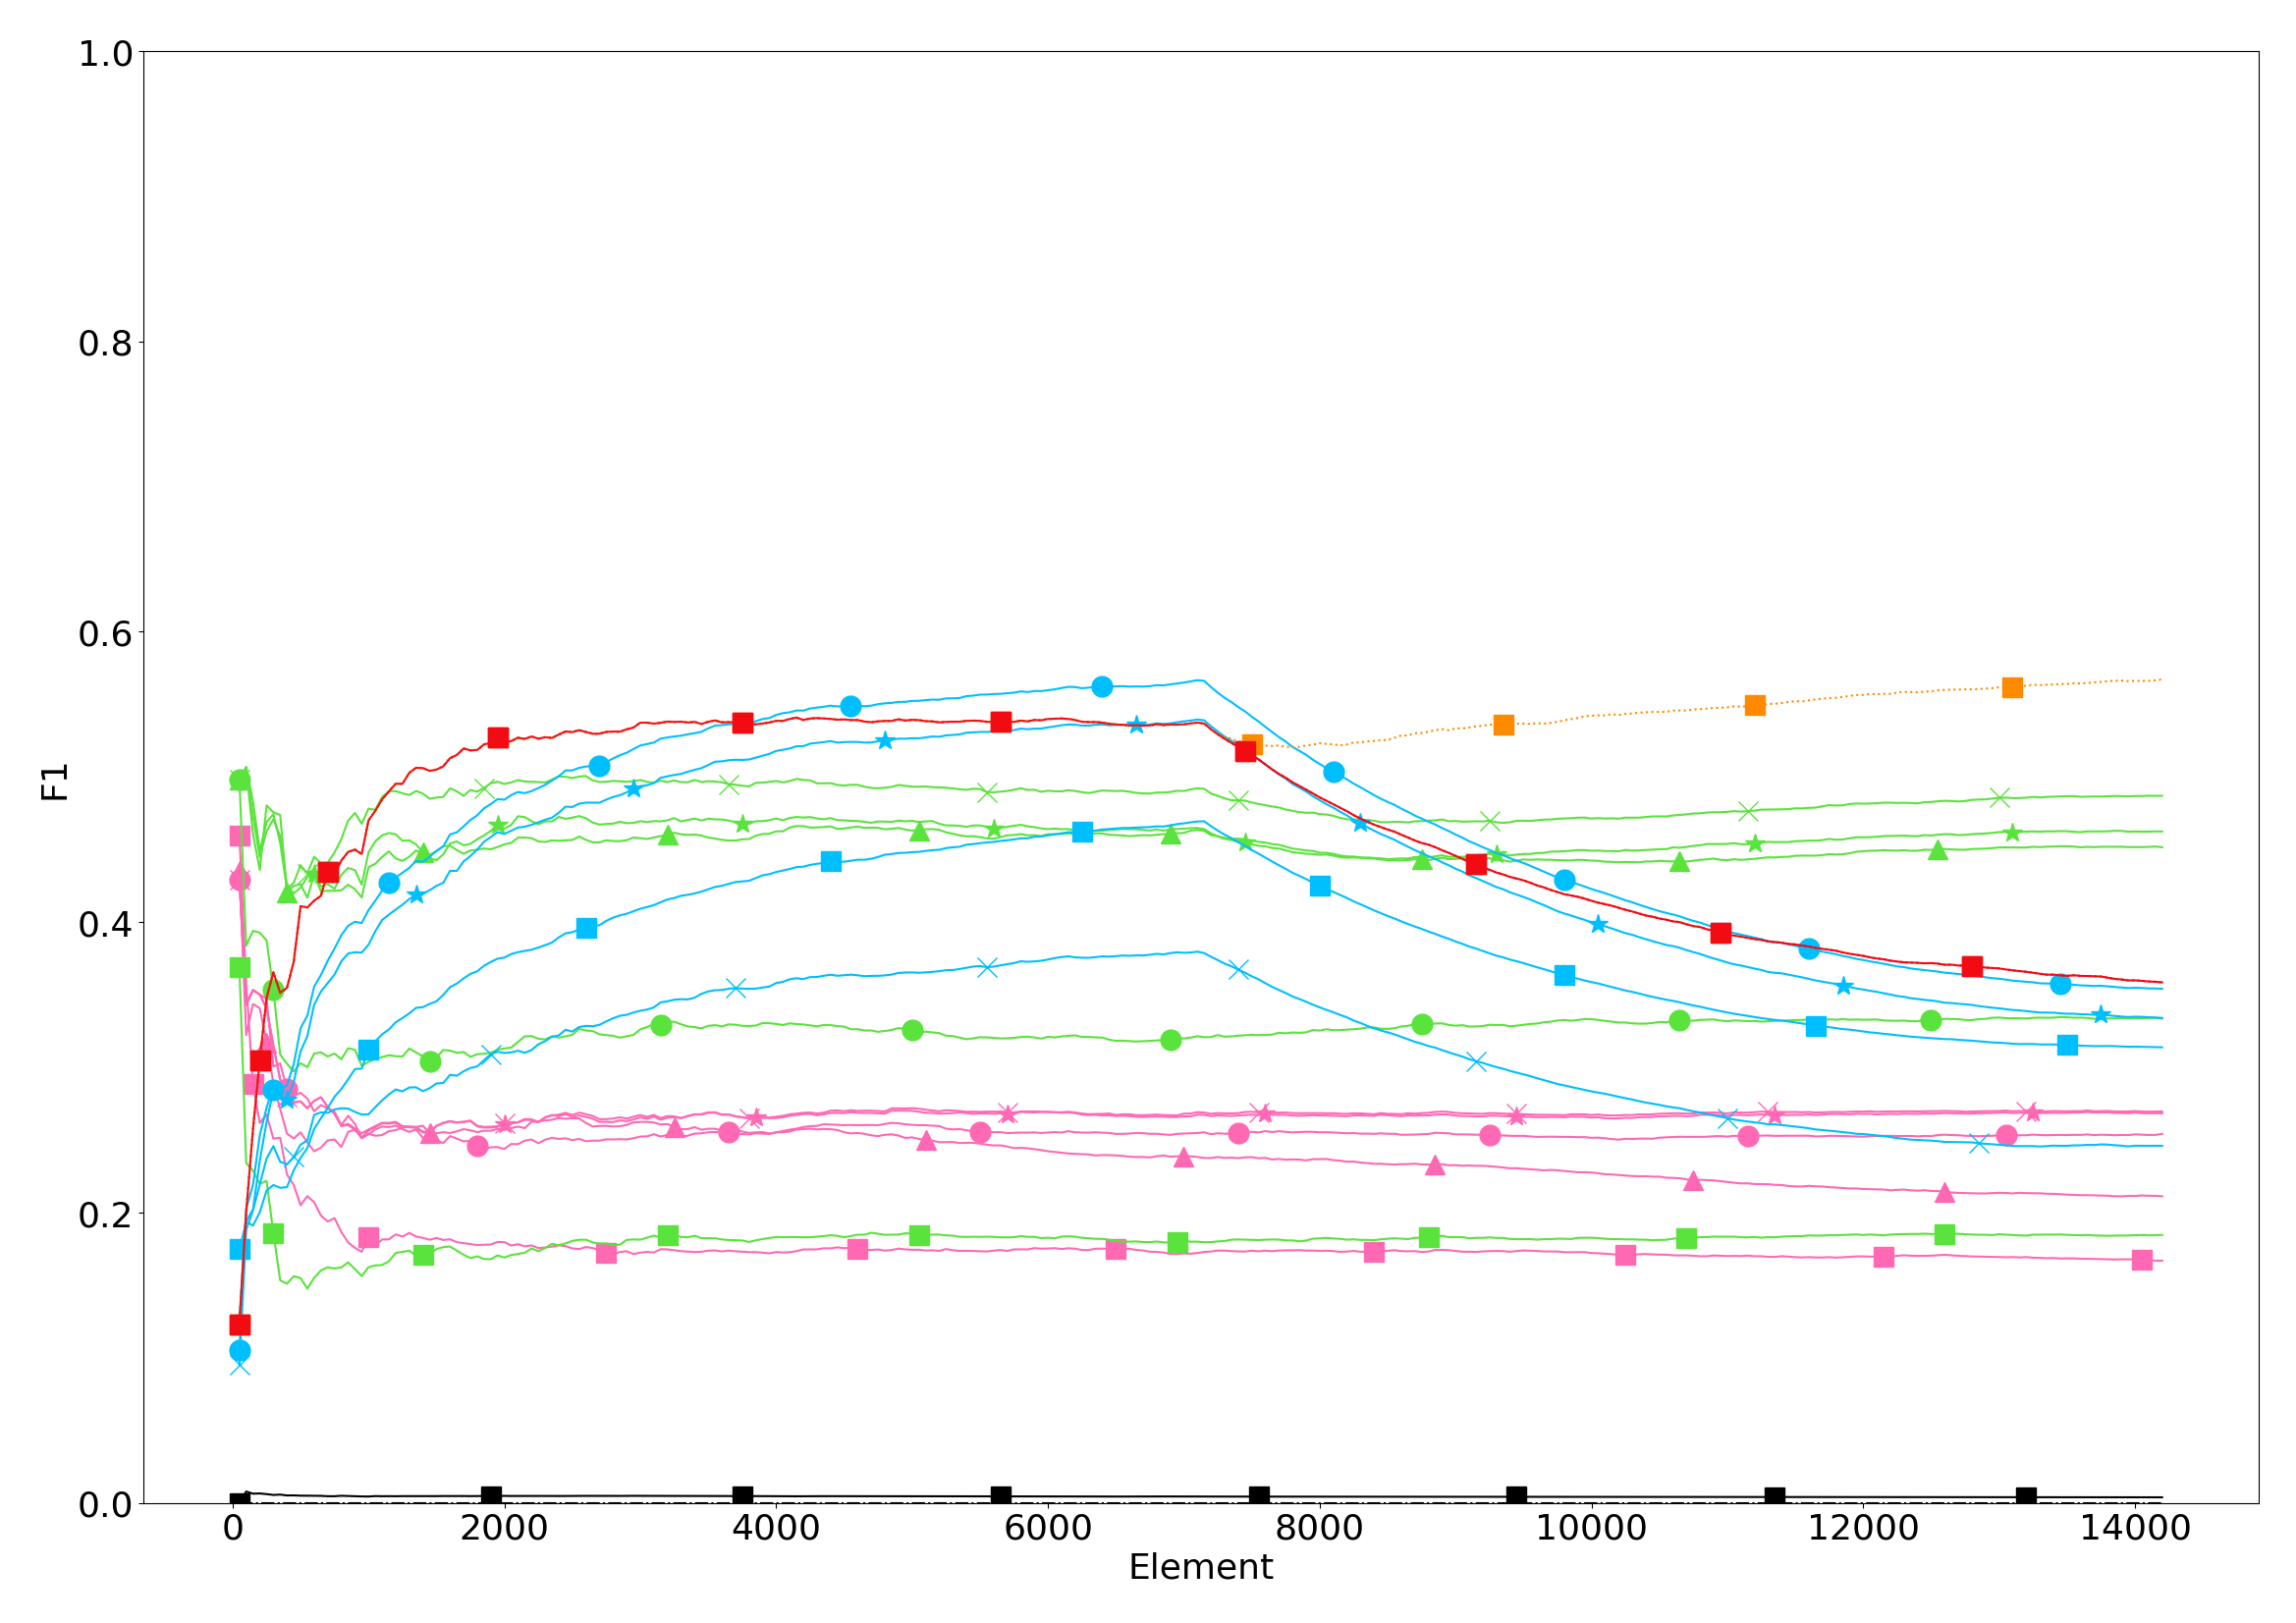
\includegraphics[width=\linewidth]{figures/results/drift_3_f1.png}
		\caption{\banosdataset (with Drift)}
		\label{fig:f1-drift}
	\end{subfigure}
	\caption{F1-scores for the six datasets. Result over 20 repetitions.}
	\label{fig:f1}
\end{figure*}

\section{Results}
This section presents our benchmarks results and the corresponding
hyperparameter tunning experiments.

\subsection{F1-score}
Figure~\ref{fig:f1} compares the F1-scores obtained by all classifiers on the
six datasets.  \naivebayes and the \hoeffdingtree outperforme the other
classifiers on the two real datasets (\banosdataset and \recofitdataset).  On
the other hand, the \mondrianforest with 5 or 10 trees achieves the best
performances on 2 synthetic datasets.  Also, the \mondrianforest is the third
classifier on the two real datasets.  Finally, the \hoeffdingtree outperform
all other classifiers on the RandomTree dataset, where it is followed by the
\mondrianforest.

F1-score values vary greatly across the datasets.  While the highest
observed F1-score is above 0.95 on the Hyperplane and RandomRBF datasets,
it barely reaches 0.65 for the \banosdataset dataset, and it remains under
0.4 on the \recofitdataset and RandomTree datasets. This trend is
consistent for all classifiers.

The StreamDM \hoeffdingtree algorithm achieves better performance than the
\naivebayes except for the \banosdataset dataset.  Both to them start close
together because the \hoeffdingtree uses a \naivebayes in its leaves.  However,
they start diverging because the \hoeffdingtree improves by reshaping its tree
structure.  This is caused by a sufficient amount of element and the difference
is more noticable when a concept drift occurs.

On all datasets, \mcnn OrpailleCC achieves better performances than \mcnn
Original. Additionally, on the datasets RandomRBF and RandomTree, the lowest
\mcnn OrpailleCC performs better than the highest \mcnn Origin \TG{not sure I
understand this sentence. Maybe add a brief explanation instead, ``presumably
due to \ldots''}.

On the real datasets (\banosdataset and \recofitdataset), the \mcnn OrpailleCC
classifier appears to be learning faster than the \mondrianforest, although
\mondrianforest catch up after a few thousand elements. 

Surprisingly, a \mondrianforest with 50 trees performs worse than with 5 or 10
trees. This is due to the fact that our \mondrianforest implementation forces a
fixed memory footprint, which limits tree growth when the allocated memory is
full. Because 50 trees fill the memory faster than 10 or 5 trees, the
classifier adaptation is blocked faster, when the trees have not learned enough
from the data.

Figure~\ref{fig:f1-banos} and Figure~\ref{fig:f1-recofit} show the F1-score
difference between two \mondrianforest. The \mondrianforest in the dark blue
plot uses twice as much memory as the on cyan plot. We notice that using more
memory induce a F1-score difference greater than 0.1 except when only one tree
is used. In which case the improvement caused by the memory is less than 0.05.

The \hoeffdingtree appears to be the most robust to concept drifts
(Figure~\ref{fig:f1-drift}), while the \mondrianforest and \naivebayes
classifier are the most impacted. \mcnn classifiers are marginally impacted.
The low resilience of \mondrianforest to concept drifts can be attributed to
two factors. First, \mondrianforest cannot update existing nodes, only add new ones.
Second, when the memory limit is reached, \mondrianforest are not able to grow
or reshape their structure anymore.

\begin{figure}
		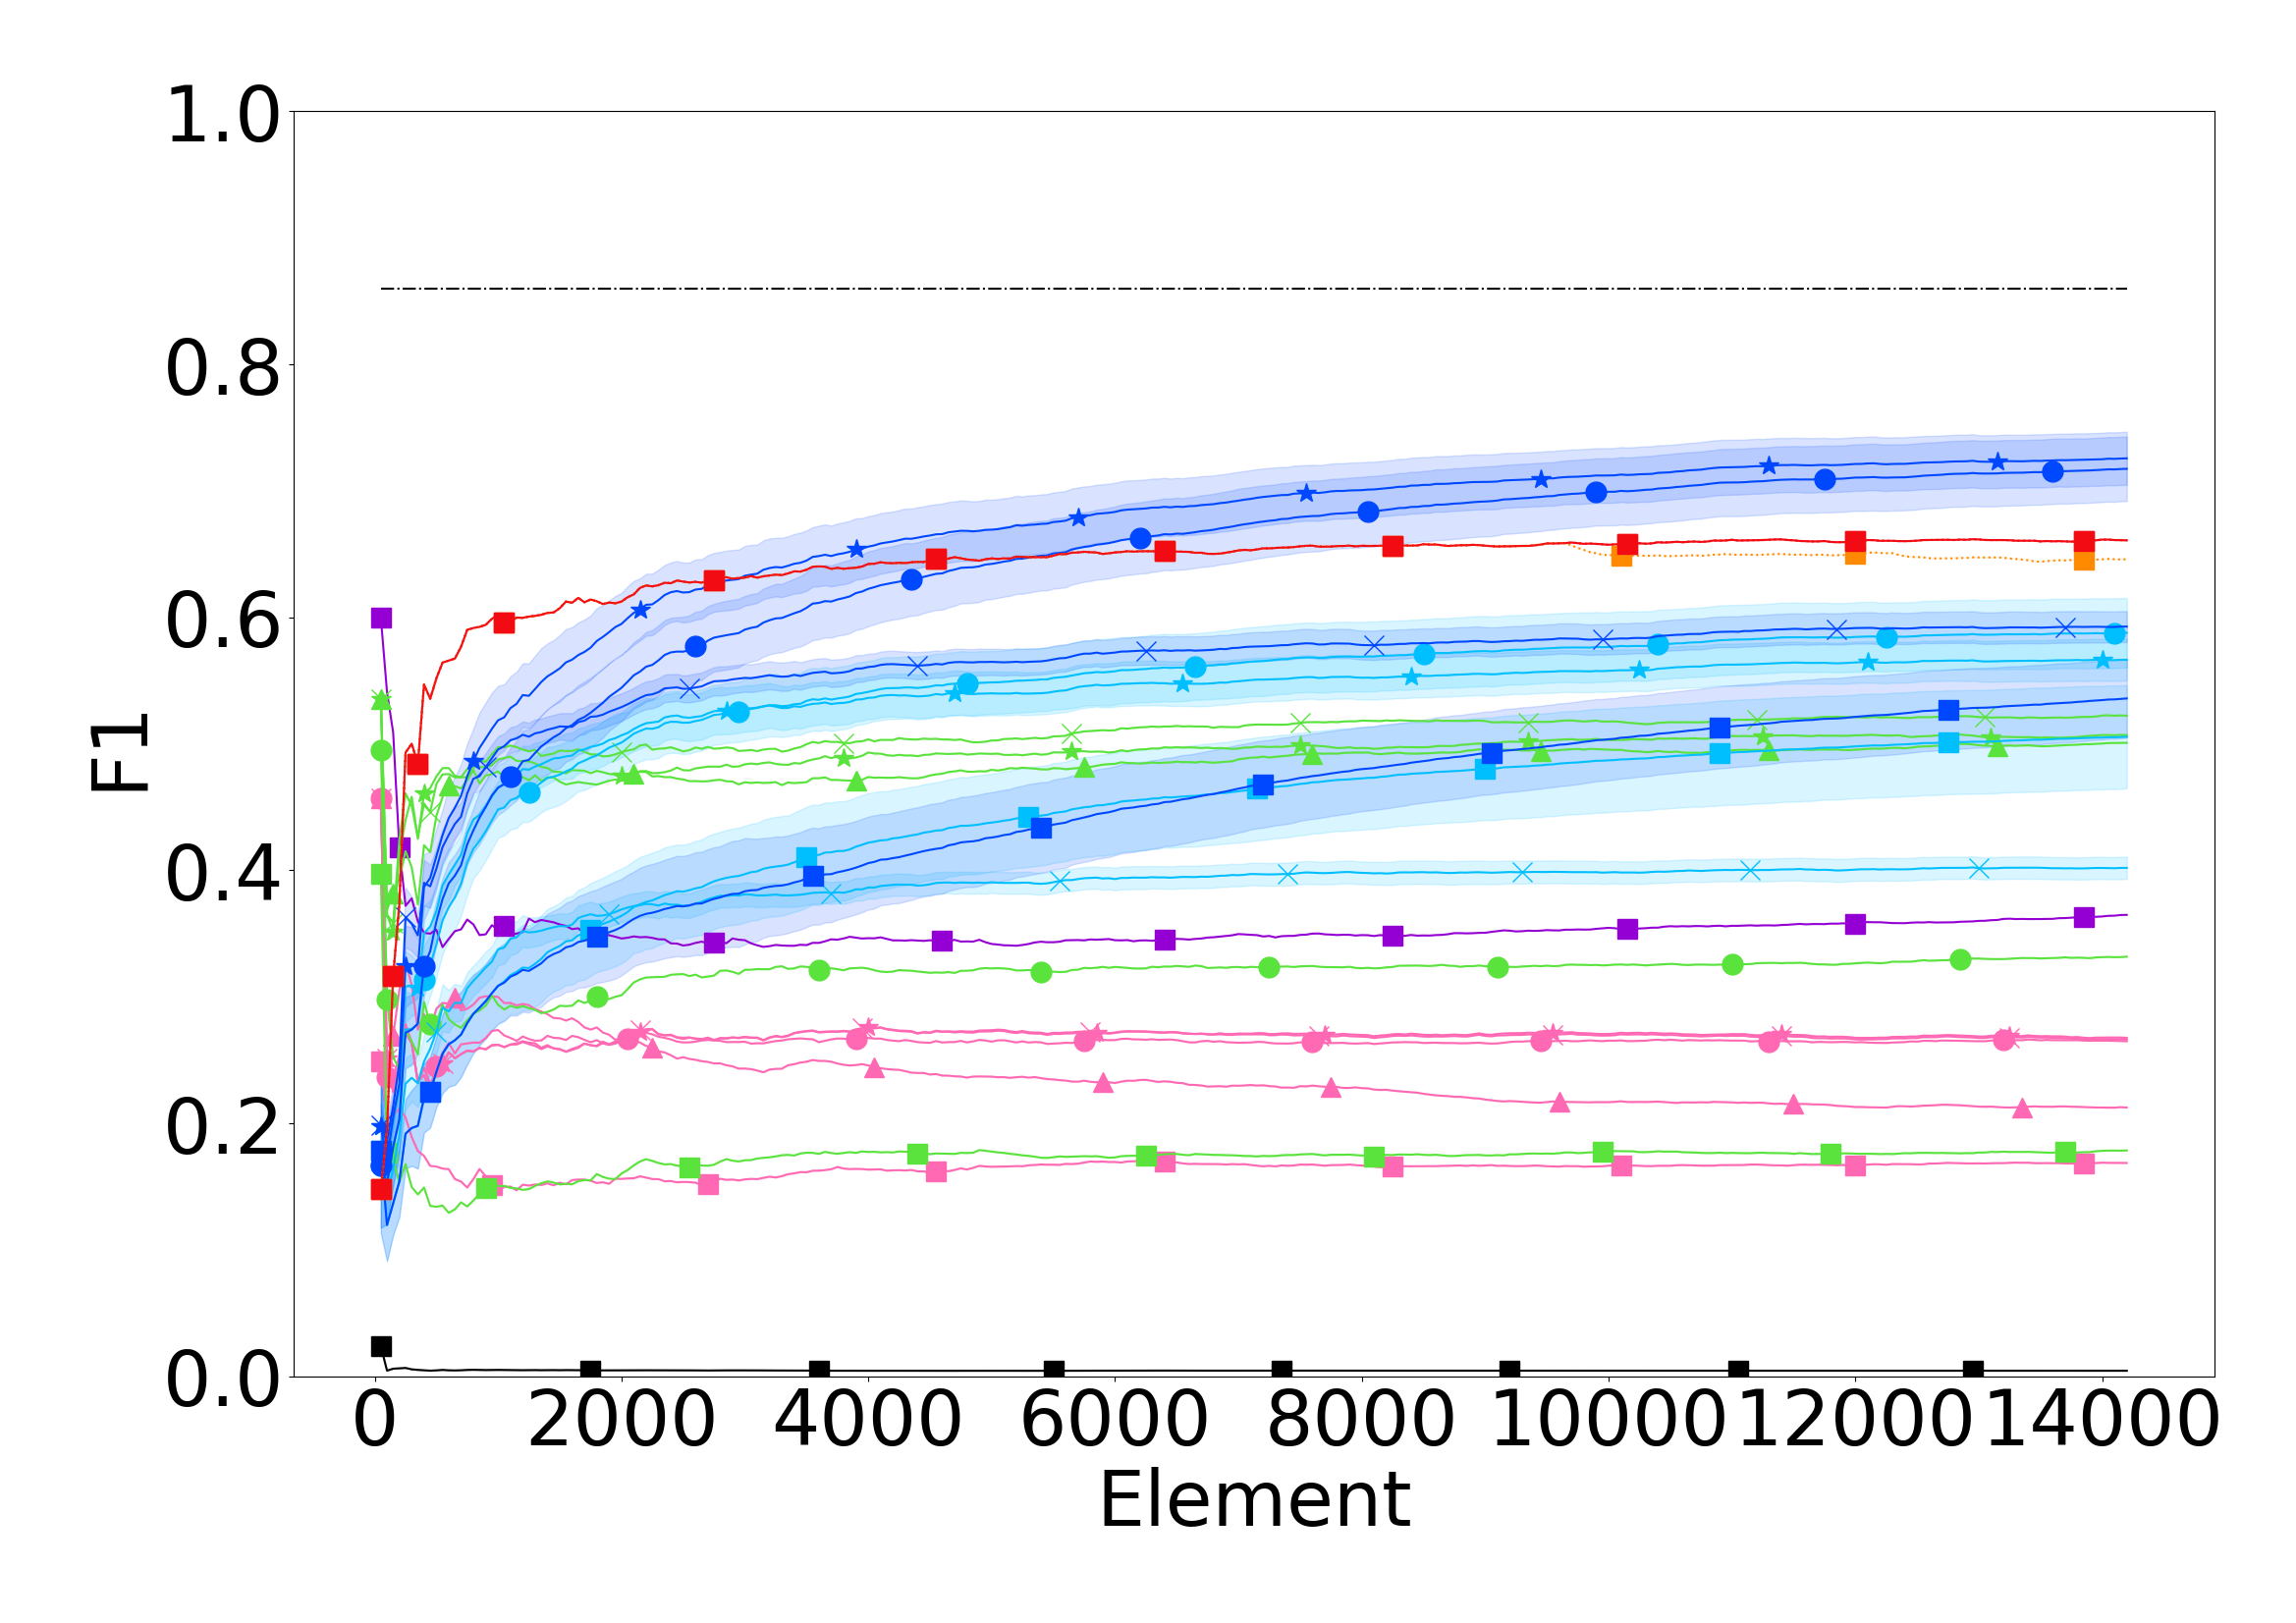
\includegraphics[width=\linewidth]{figures/results/banos_6_f1_std.png}
		\caption{F1-score variance on \banosdataset dataset. Some classifiers
		have been removed to make the Figure clearer (\mcnn Origin,
		\hoeffdingtree, some of the \mcnn OrpailleCC)}
		\label{fig:f1-variance}
\end{figure}

Figure~\ref{fig:f1-variance} shows the F1-score variance for the classifiers.
Only \mondrianforest has variance since it is the only one involving
randomness. Hence, we removed so classifier from the Figure to make it clearer.
On Figure~\ref{fig:f1-variance} we notice that \mondrianforest variance
decreases with the number of tree. The higher the tree count, the lower the
variance. Finally, we notice that the \mondrianforest variance with double
memory covers the \naivebayes lines. Therefore, some \mondrianforest run
achieves better F1-score than the \naivebayes.

Figure~\ref{fig:f1-banos} shows that the F1-score of the \FNN
is around 0.3. Therefore, it remains better than \mcnn Origin but it is quite
low compare to other classifiers with the same dataset.

Finally, we notice that the StreamDM and OrpailleCC implementations of
\naivebayes remain close on the two real datasets: \banosdataset and
\recofitdataset.  This suggests that the two implementations are not similar,
but SreamDM implements additional mechanisms \TG{this is too vague}.

\begin{figure*}
	\begin{subfigure}[t]{.49\linewidth}
		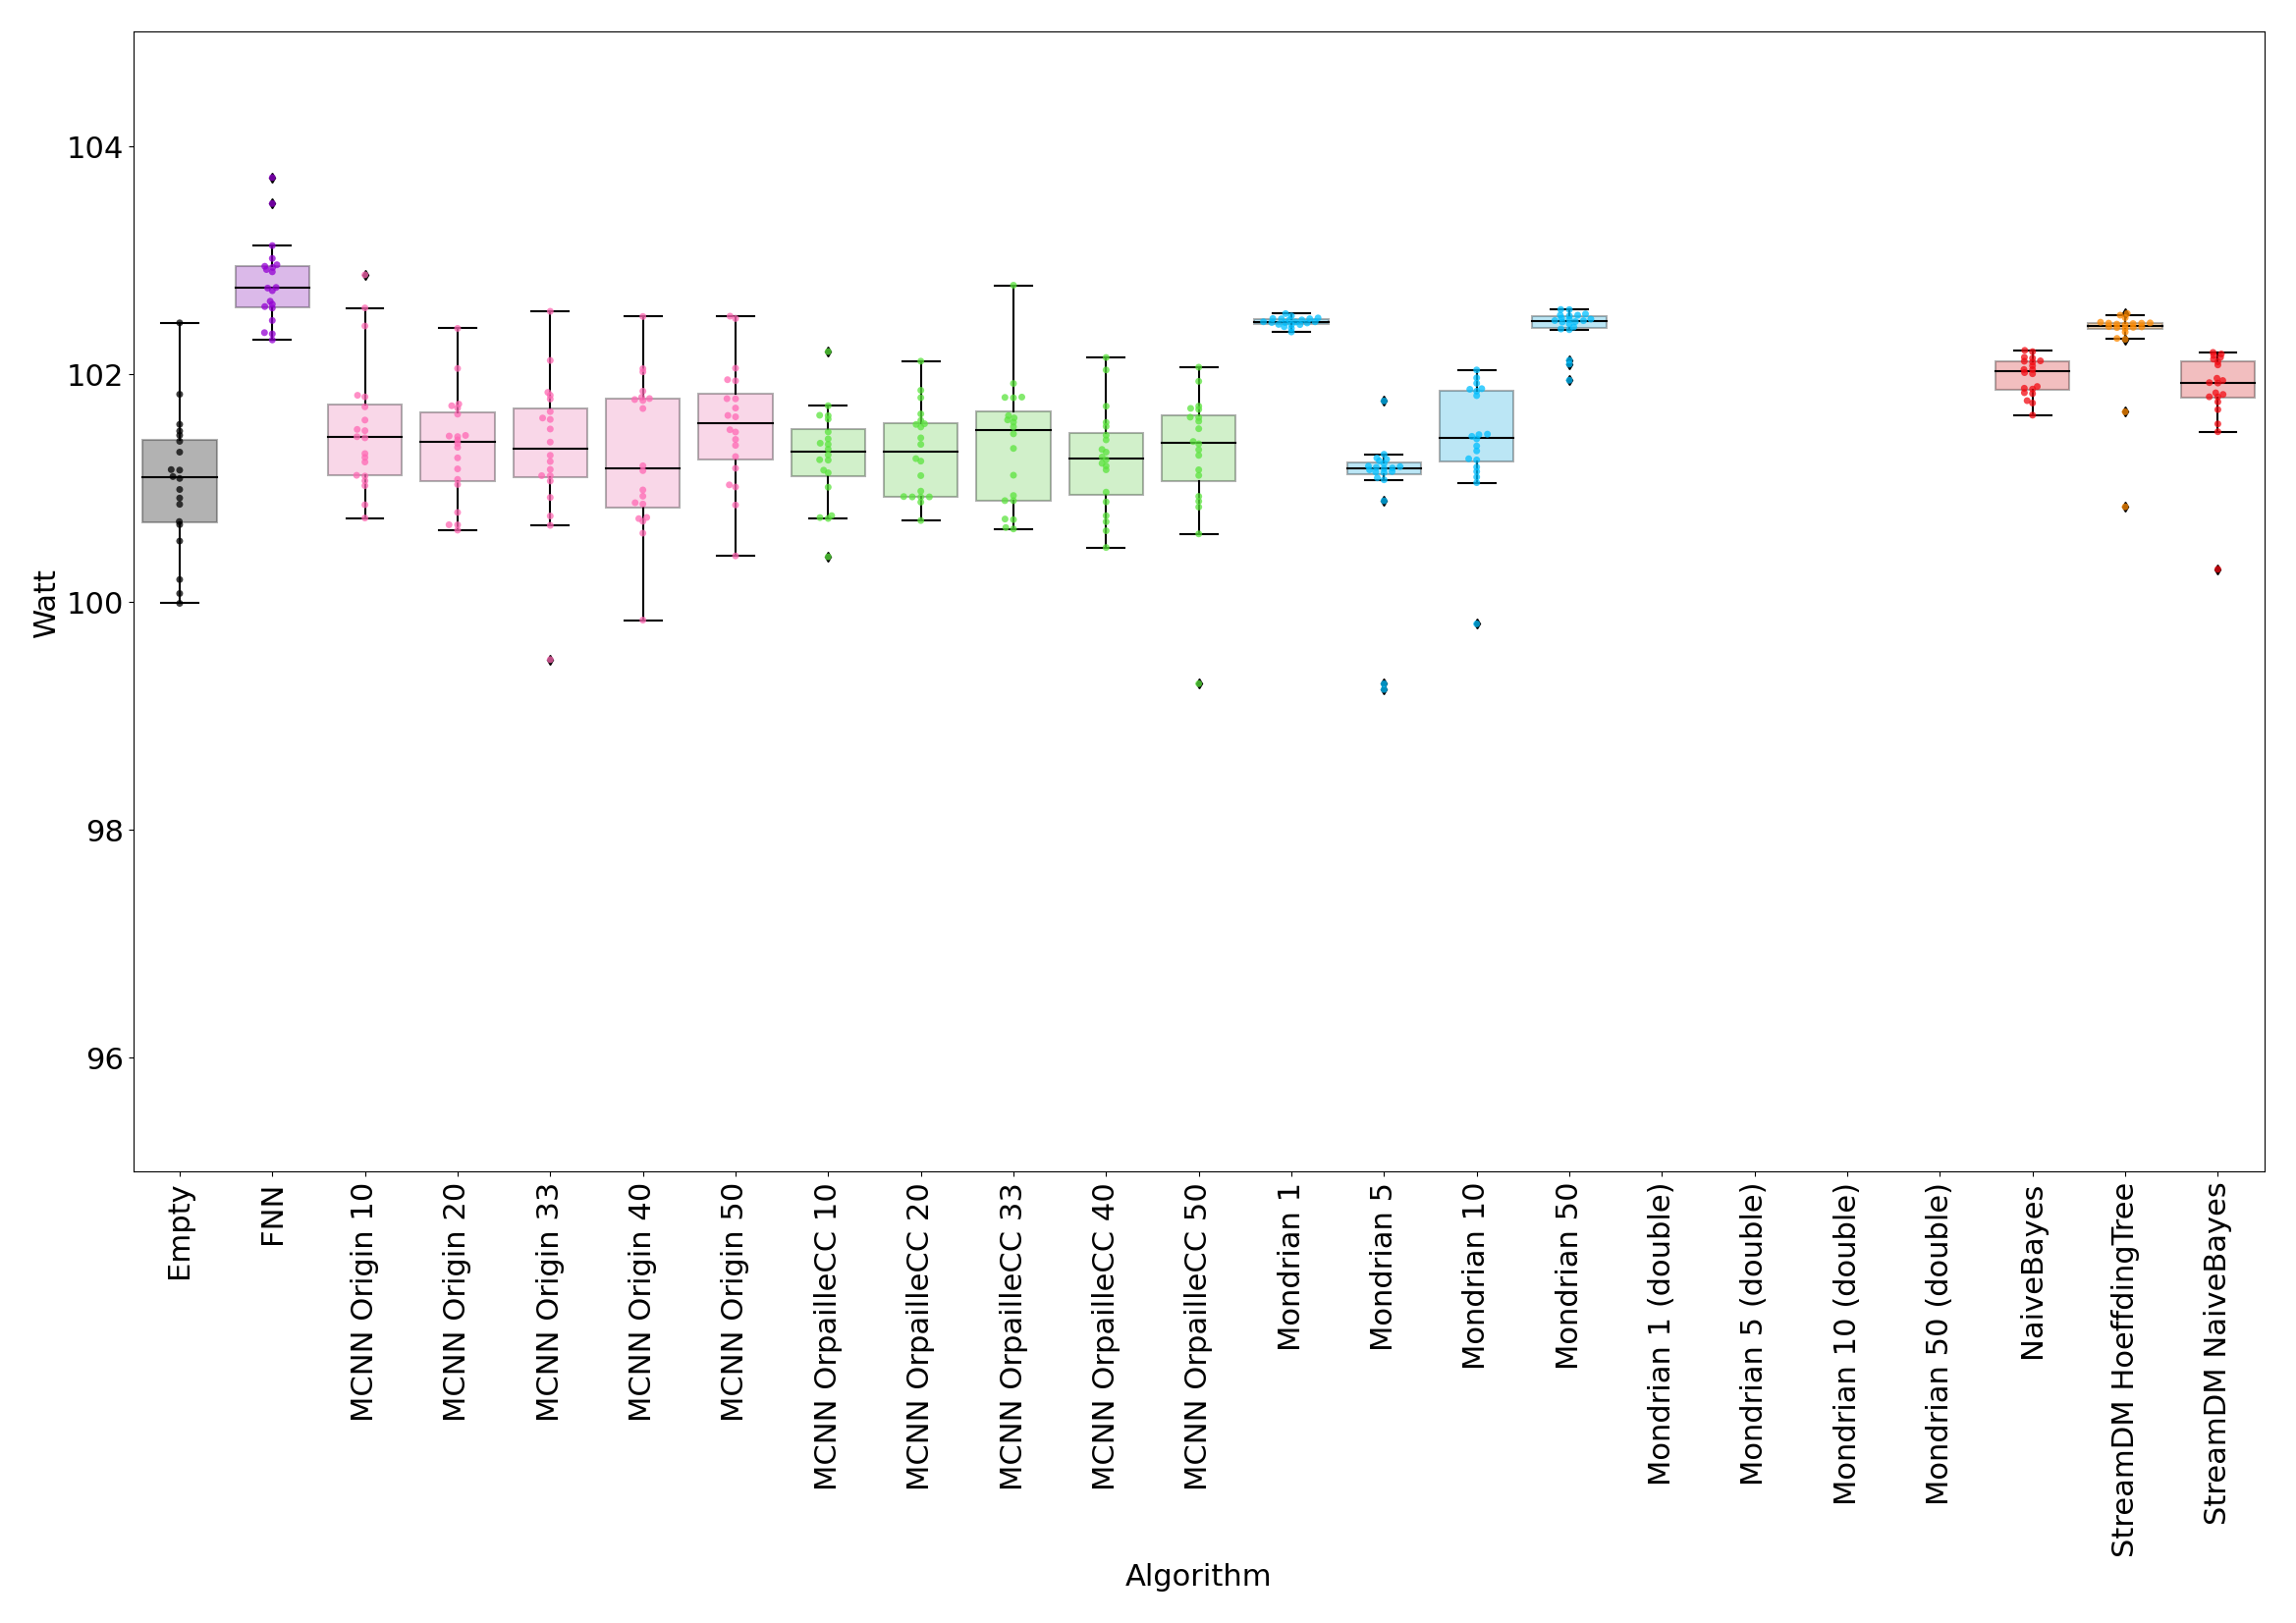
\includegraphics[width=\linewidth]{figures/results/banos_3_watt.png}
		\caption{\banosdataset}
		\label{fig:power-banos}
	\end{subfigure}
	\hfill
	\begin{subfigure}[t]{.49\linewidth}
		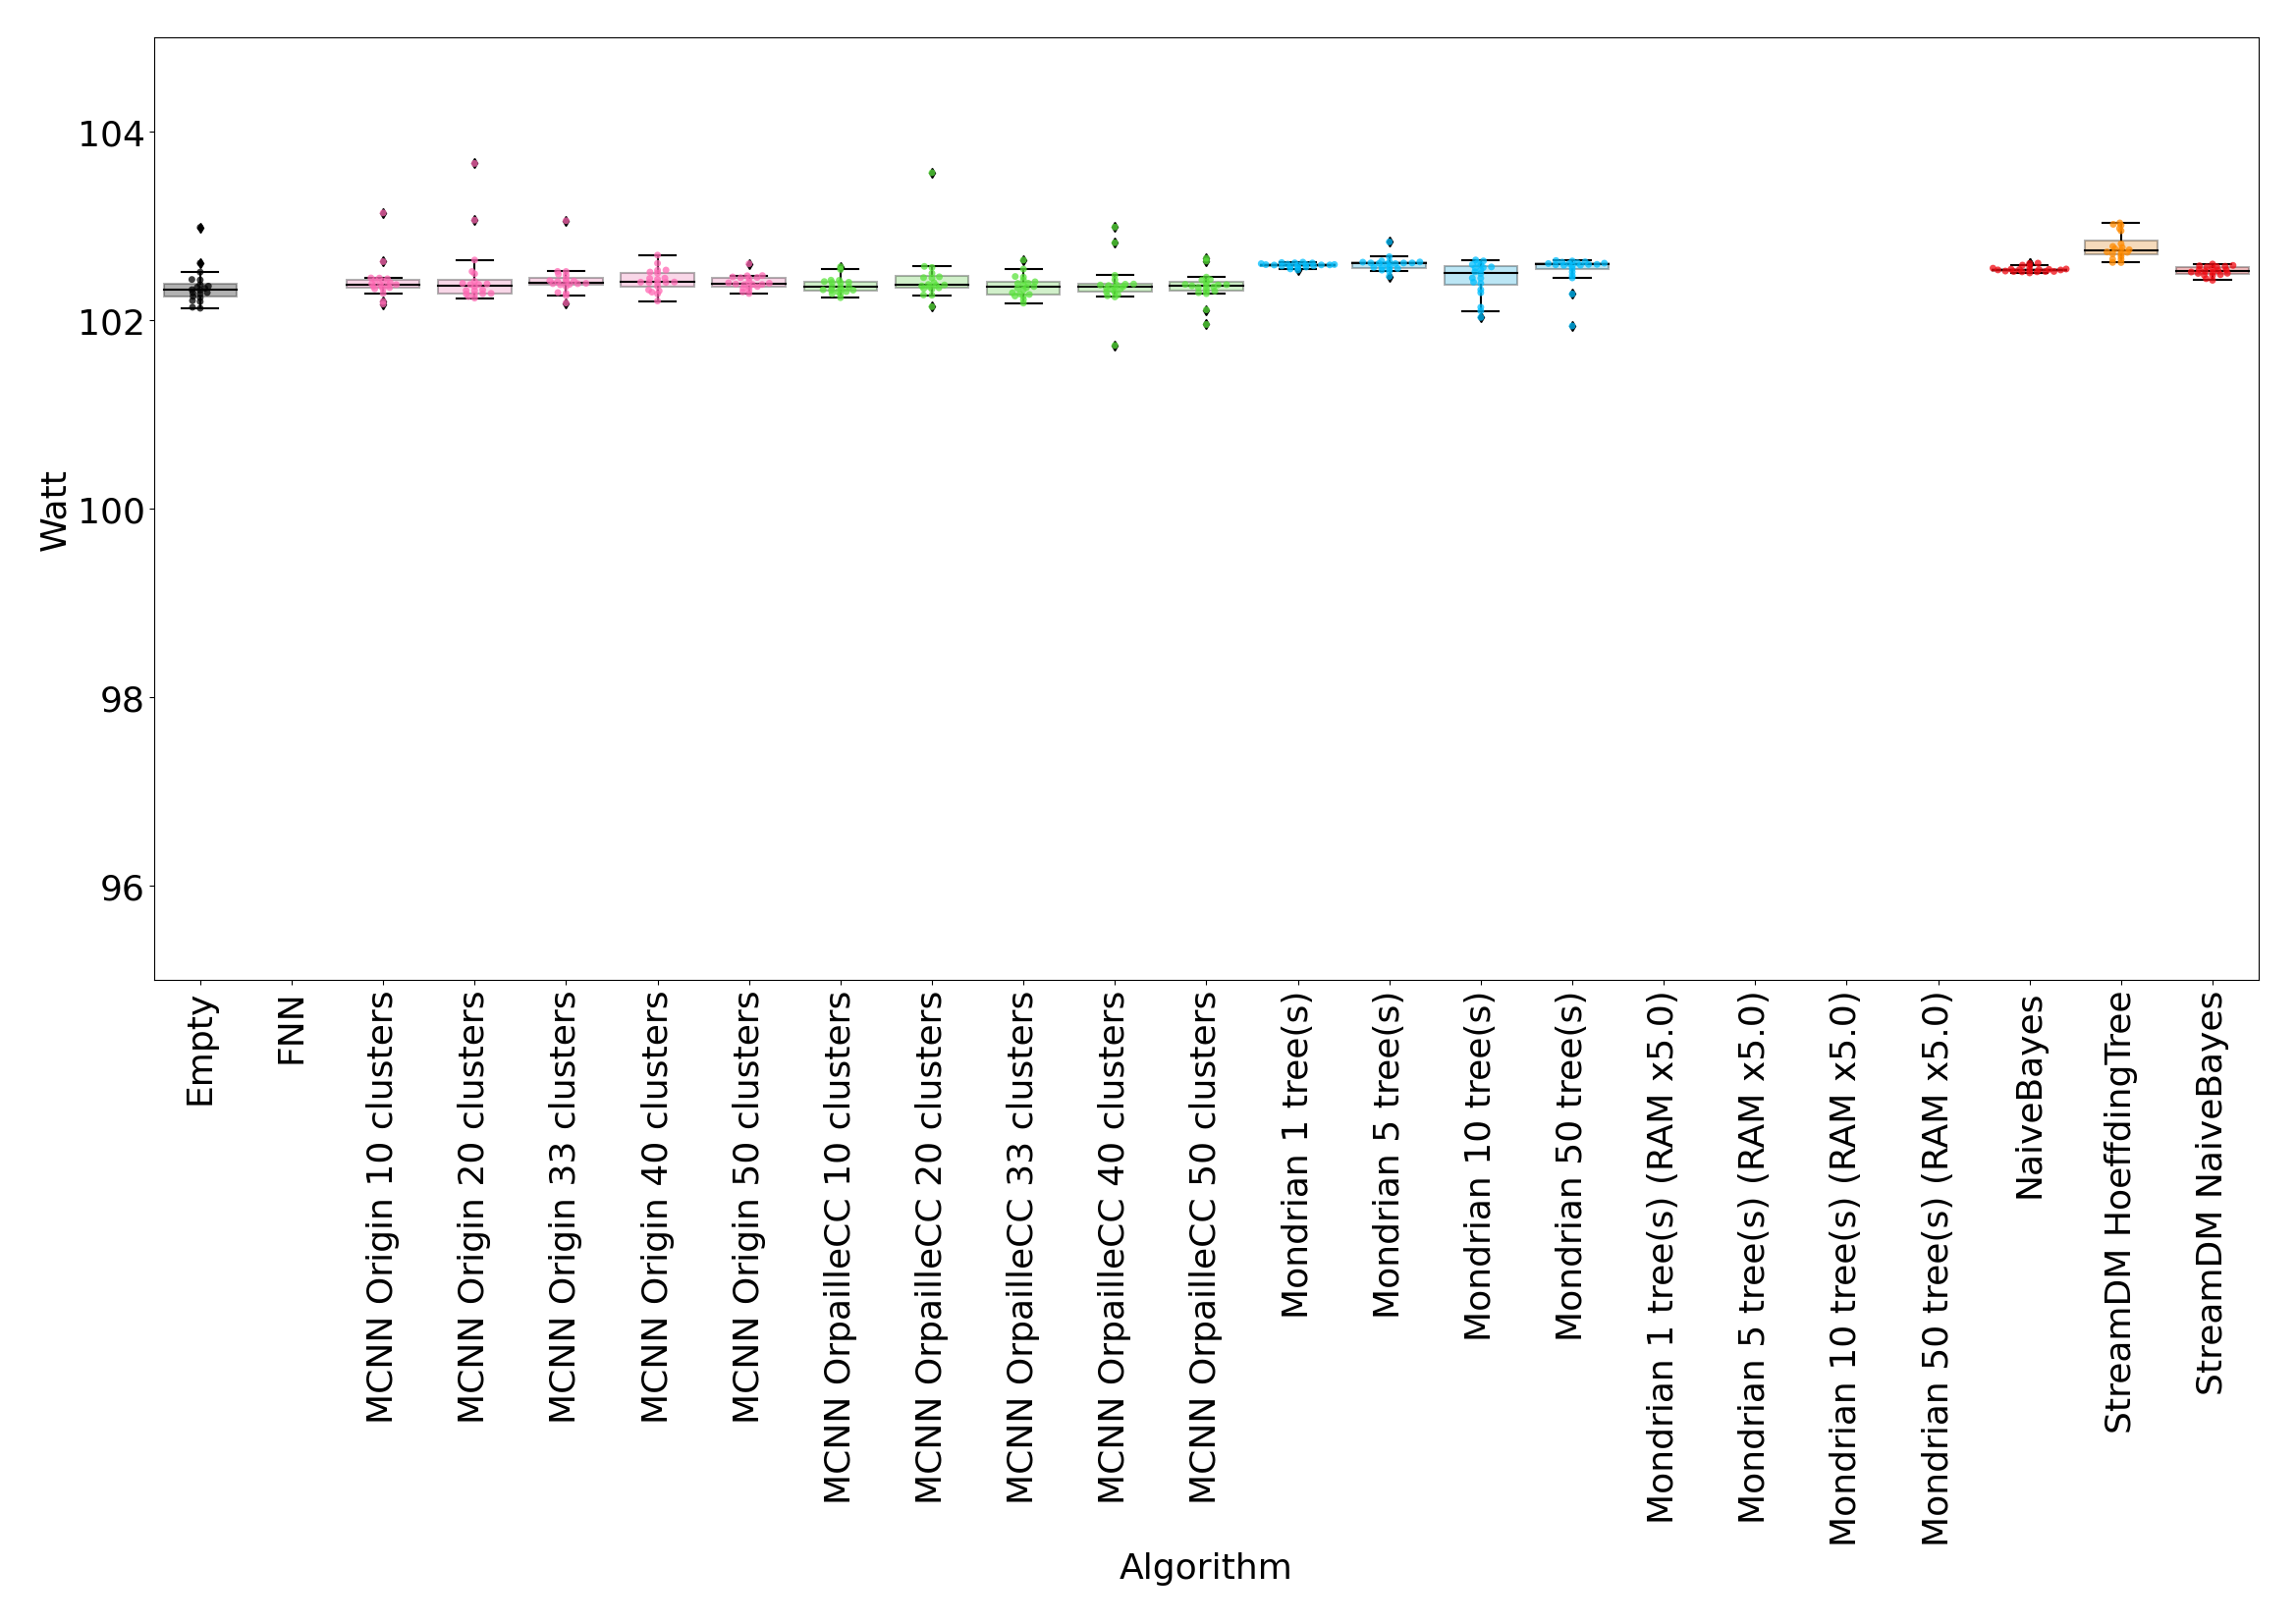
\includegraphics[width=\linewidth]{figures/results/recofit_3_watt.png}
		\caption{\recofitdataset}
		\label{fig:power-recofit}
	\end{subfigure}\\
	\begin{subfigure}[t]{.49\linewidth}
		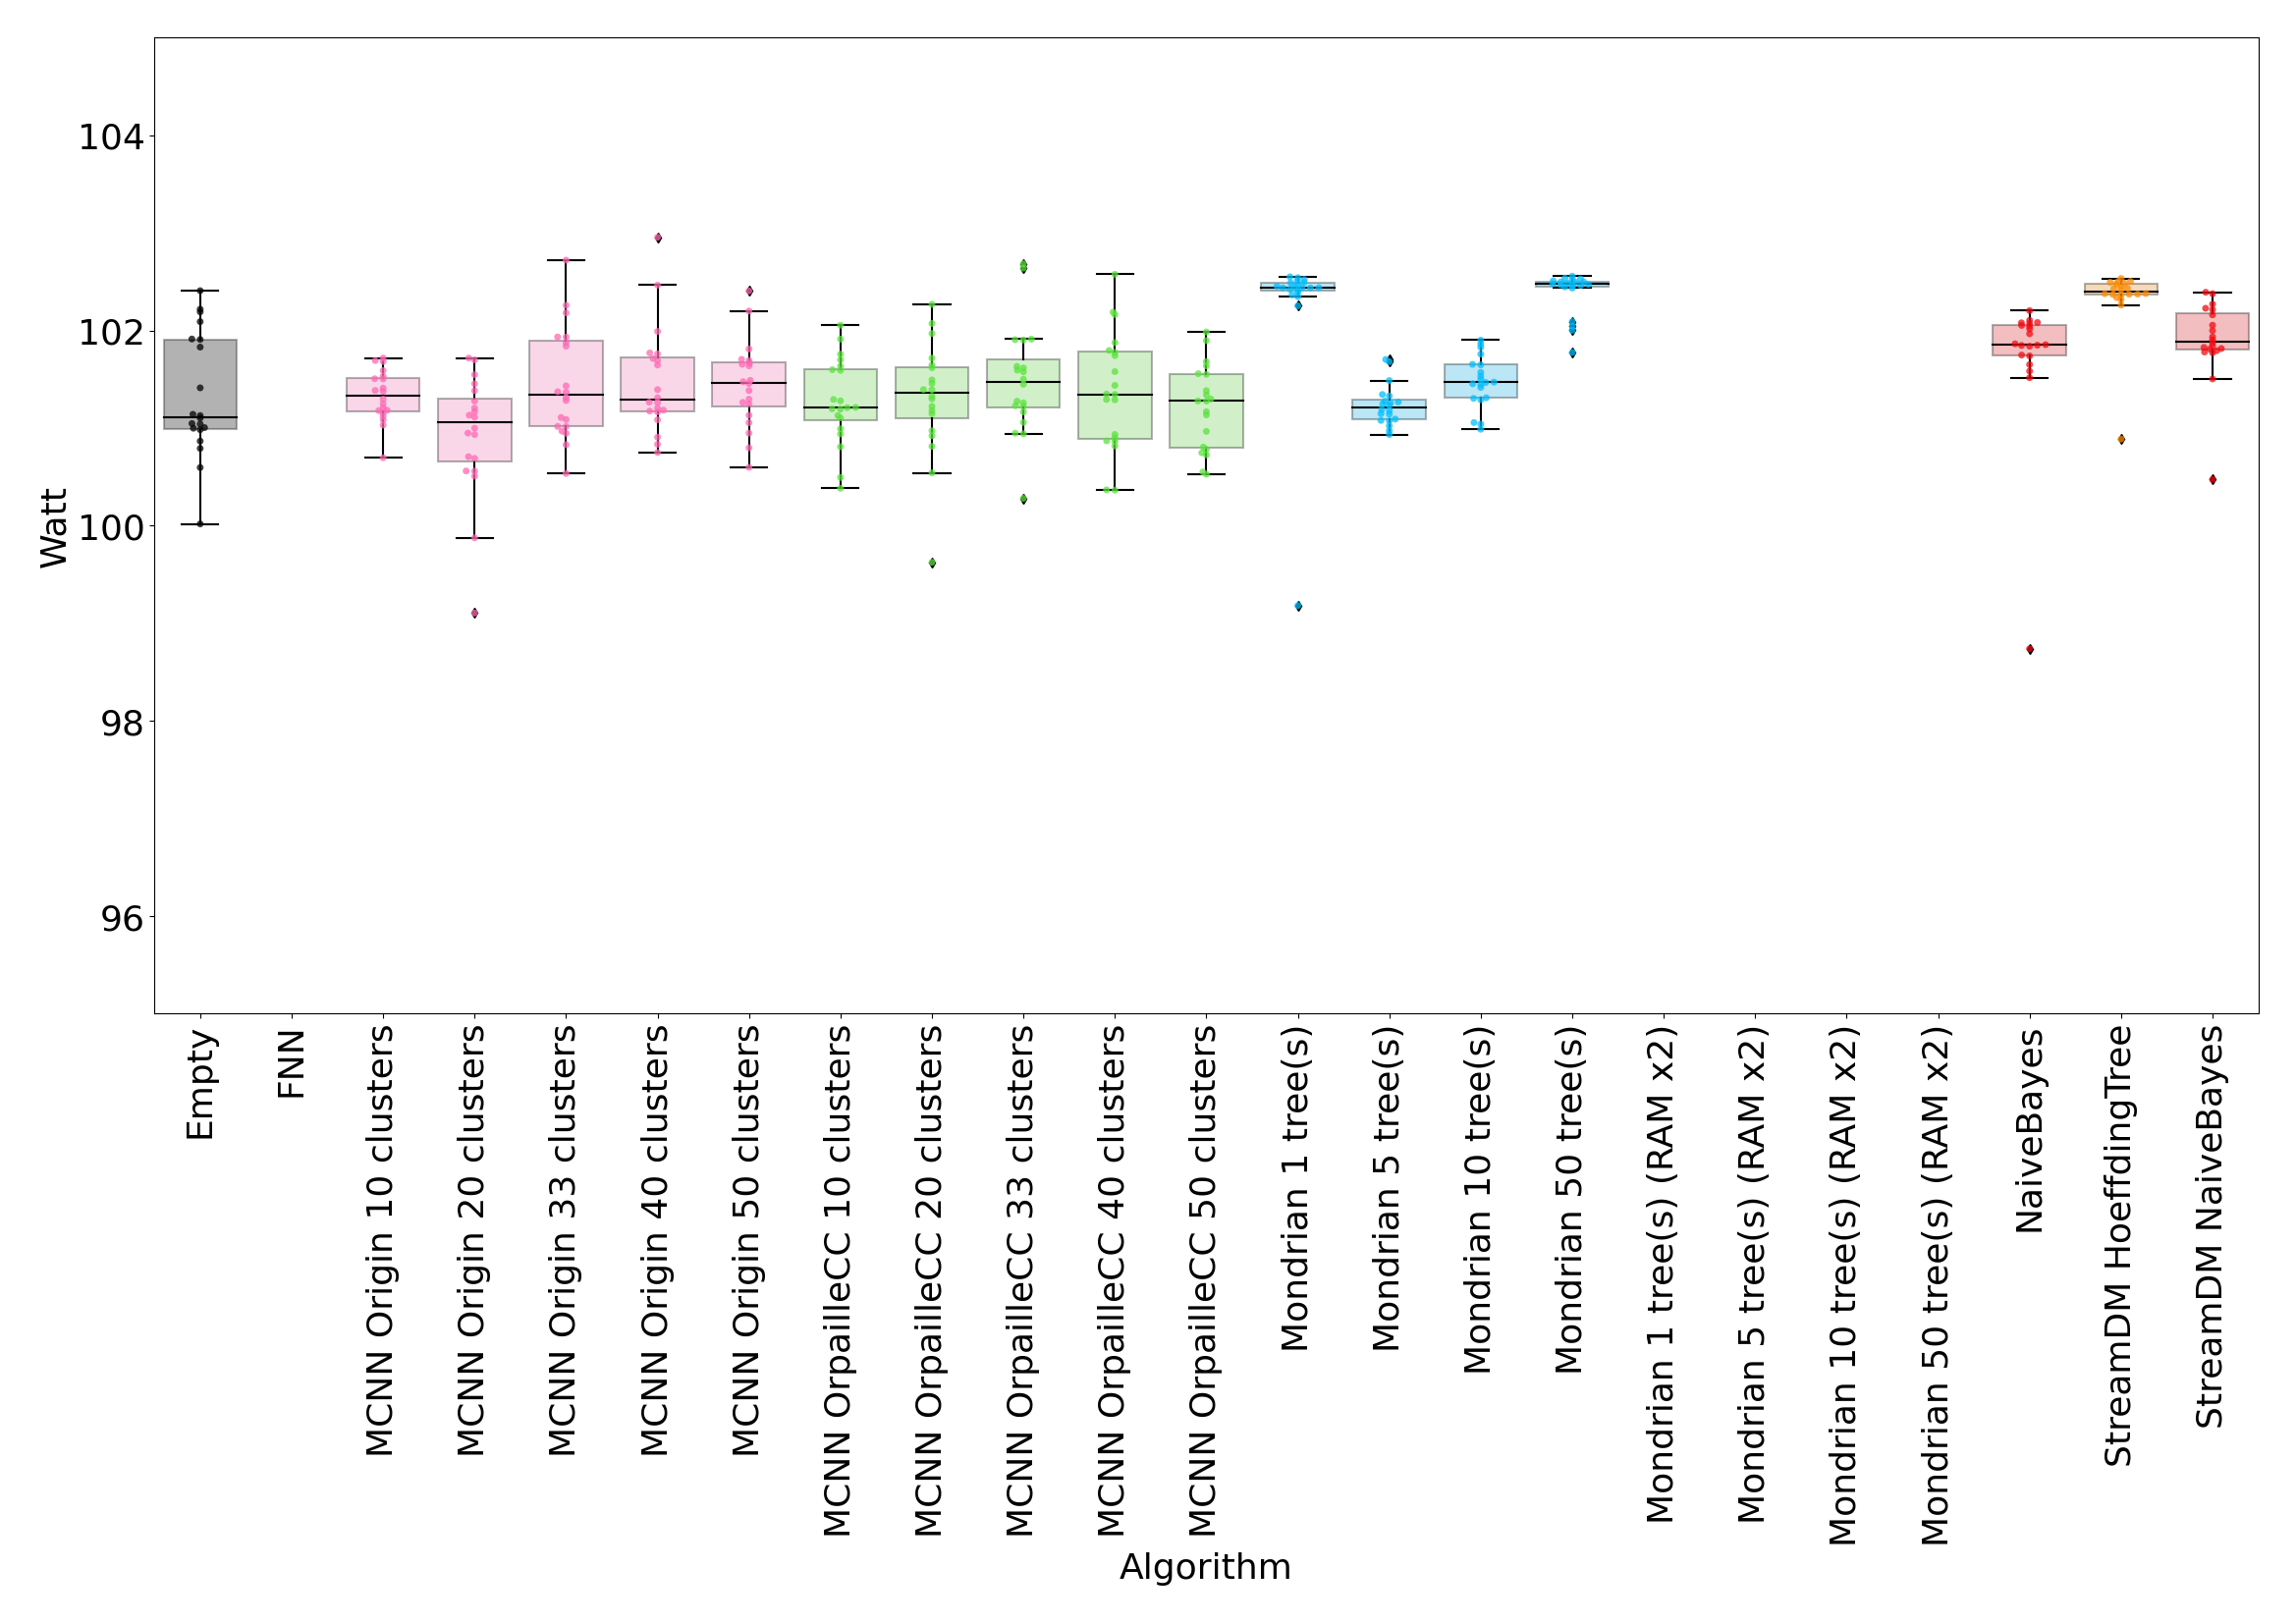
\includegraphics[width=\linewidth]{figures/results/drift_3_watt.png}
		\caption{\banosdataset with drift.}
		\label{fig:power-drift}
	\end{subfigure}
	\hfill
	\begin{subfigure}[t]{.49\linewidth}
		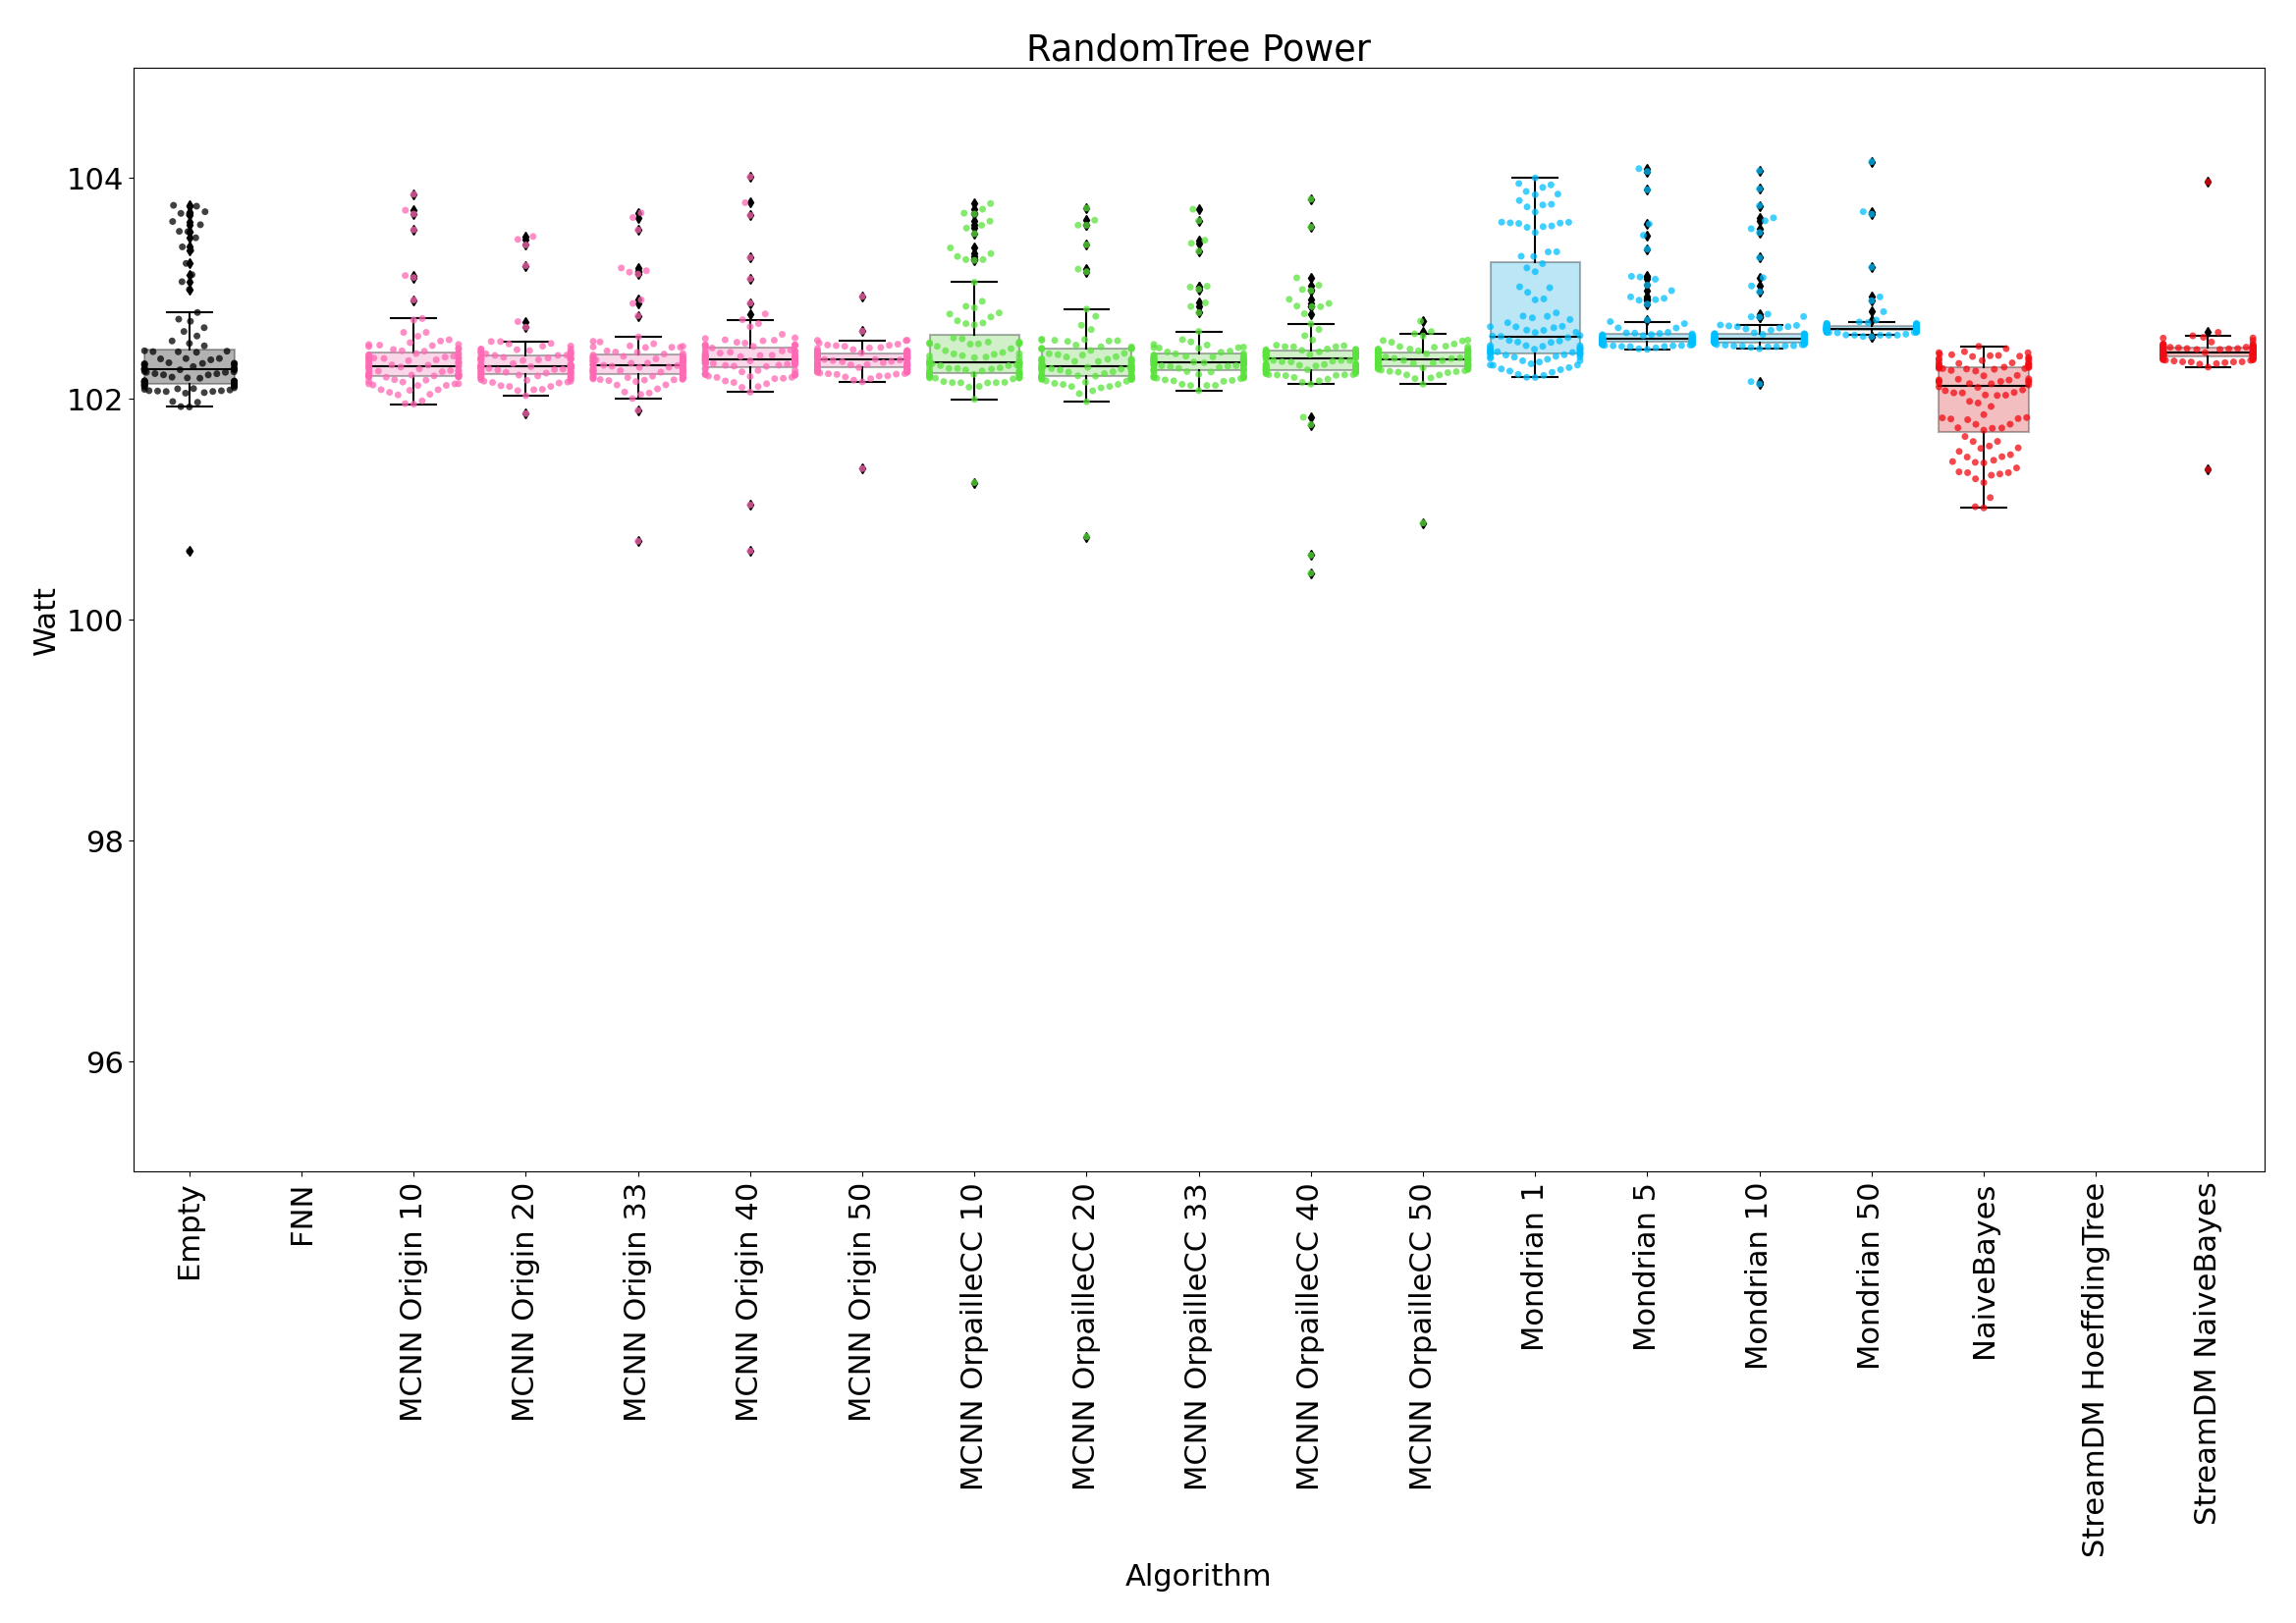
\includegraphics[width=\linewidth]{figures/results/dataset_3_watt.png}
		\caption{RandomTree}
		\label{fig:power-dataset_3}
	\end{subfigure}
	\caption{Power usage for four datasets.}
	\label{fig:power}
\end{figure*}
\subsection{Power}
\label{sec:result-power}
Figure~\ref{fig:power} shows the power usage of each classifier on four
datasets. Since all classifiers
exhibit comparable power consumptions, close to 102~W, we decided to show only
four of them.


\subsection{Runtime}
Figure~\ref{fig:runtime} shows the runtime of classifiers for the two real
datasets.
\mondrianforest are the slowest classifier, in particular for 50 trees. The
second slowest classifier is the \hoeffdingtree, which compares with the 1-tree
\mondrianforest. The \hoeffdingtree is followed by the two \naivebayes
implementations, which is not surprising since \naivebayes classifiers are used
in the leaves of the \hoeffdingtree. The \mcnn classifiers are the fastest
ones, with a runtime very close to the empty classifier.

We observe that \naivebayes from StreamDM is slightly faster than the one
from OrpailleCC \TG{I think they are quite comparable in fact. You should
explain that this makes the comparison between hoeffding tree and mondrian
fair even though they are implemented differently.}.

\begin{figure*}
	\begin{subfigure}[t]{.49\linewidth}
		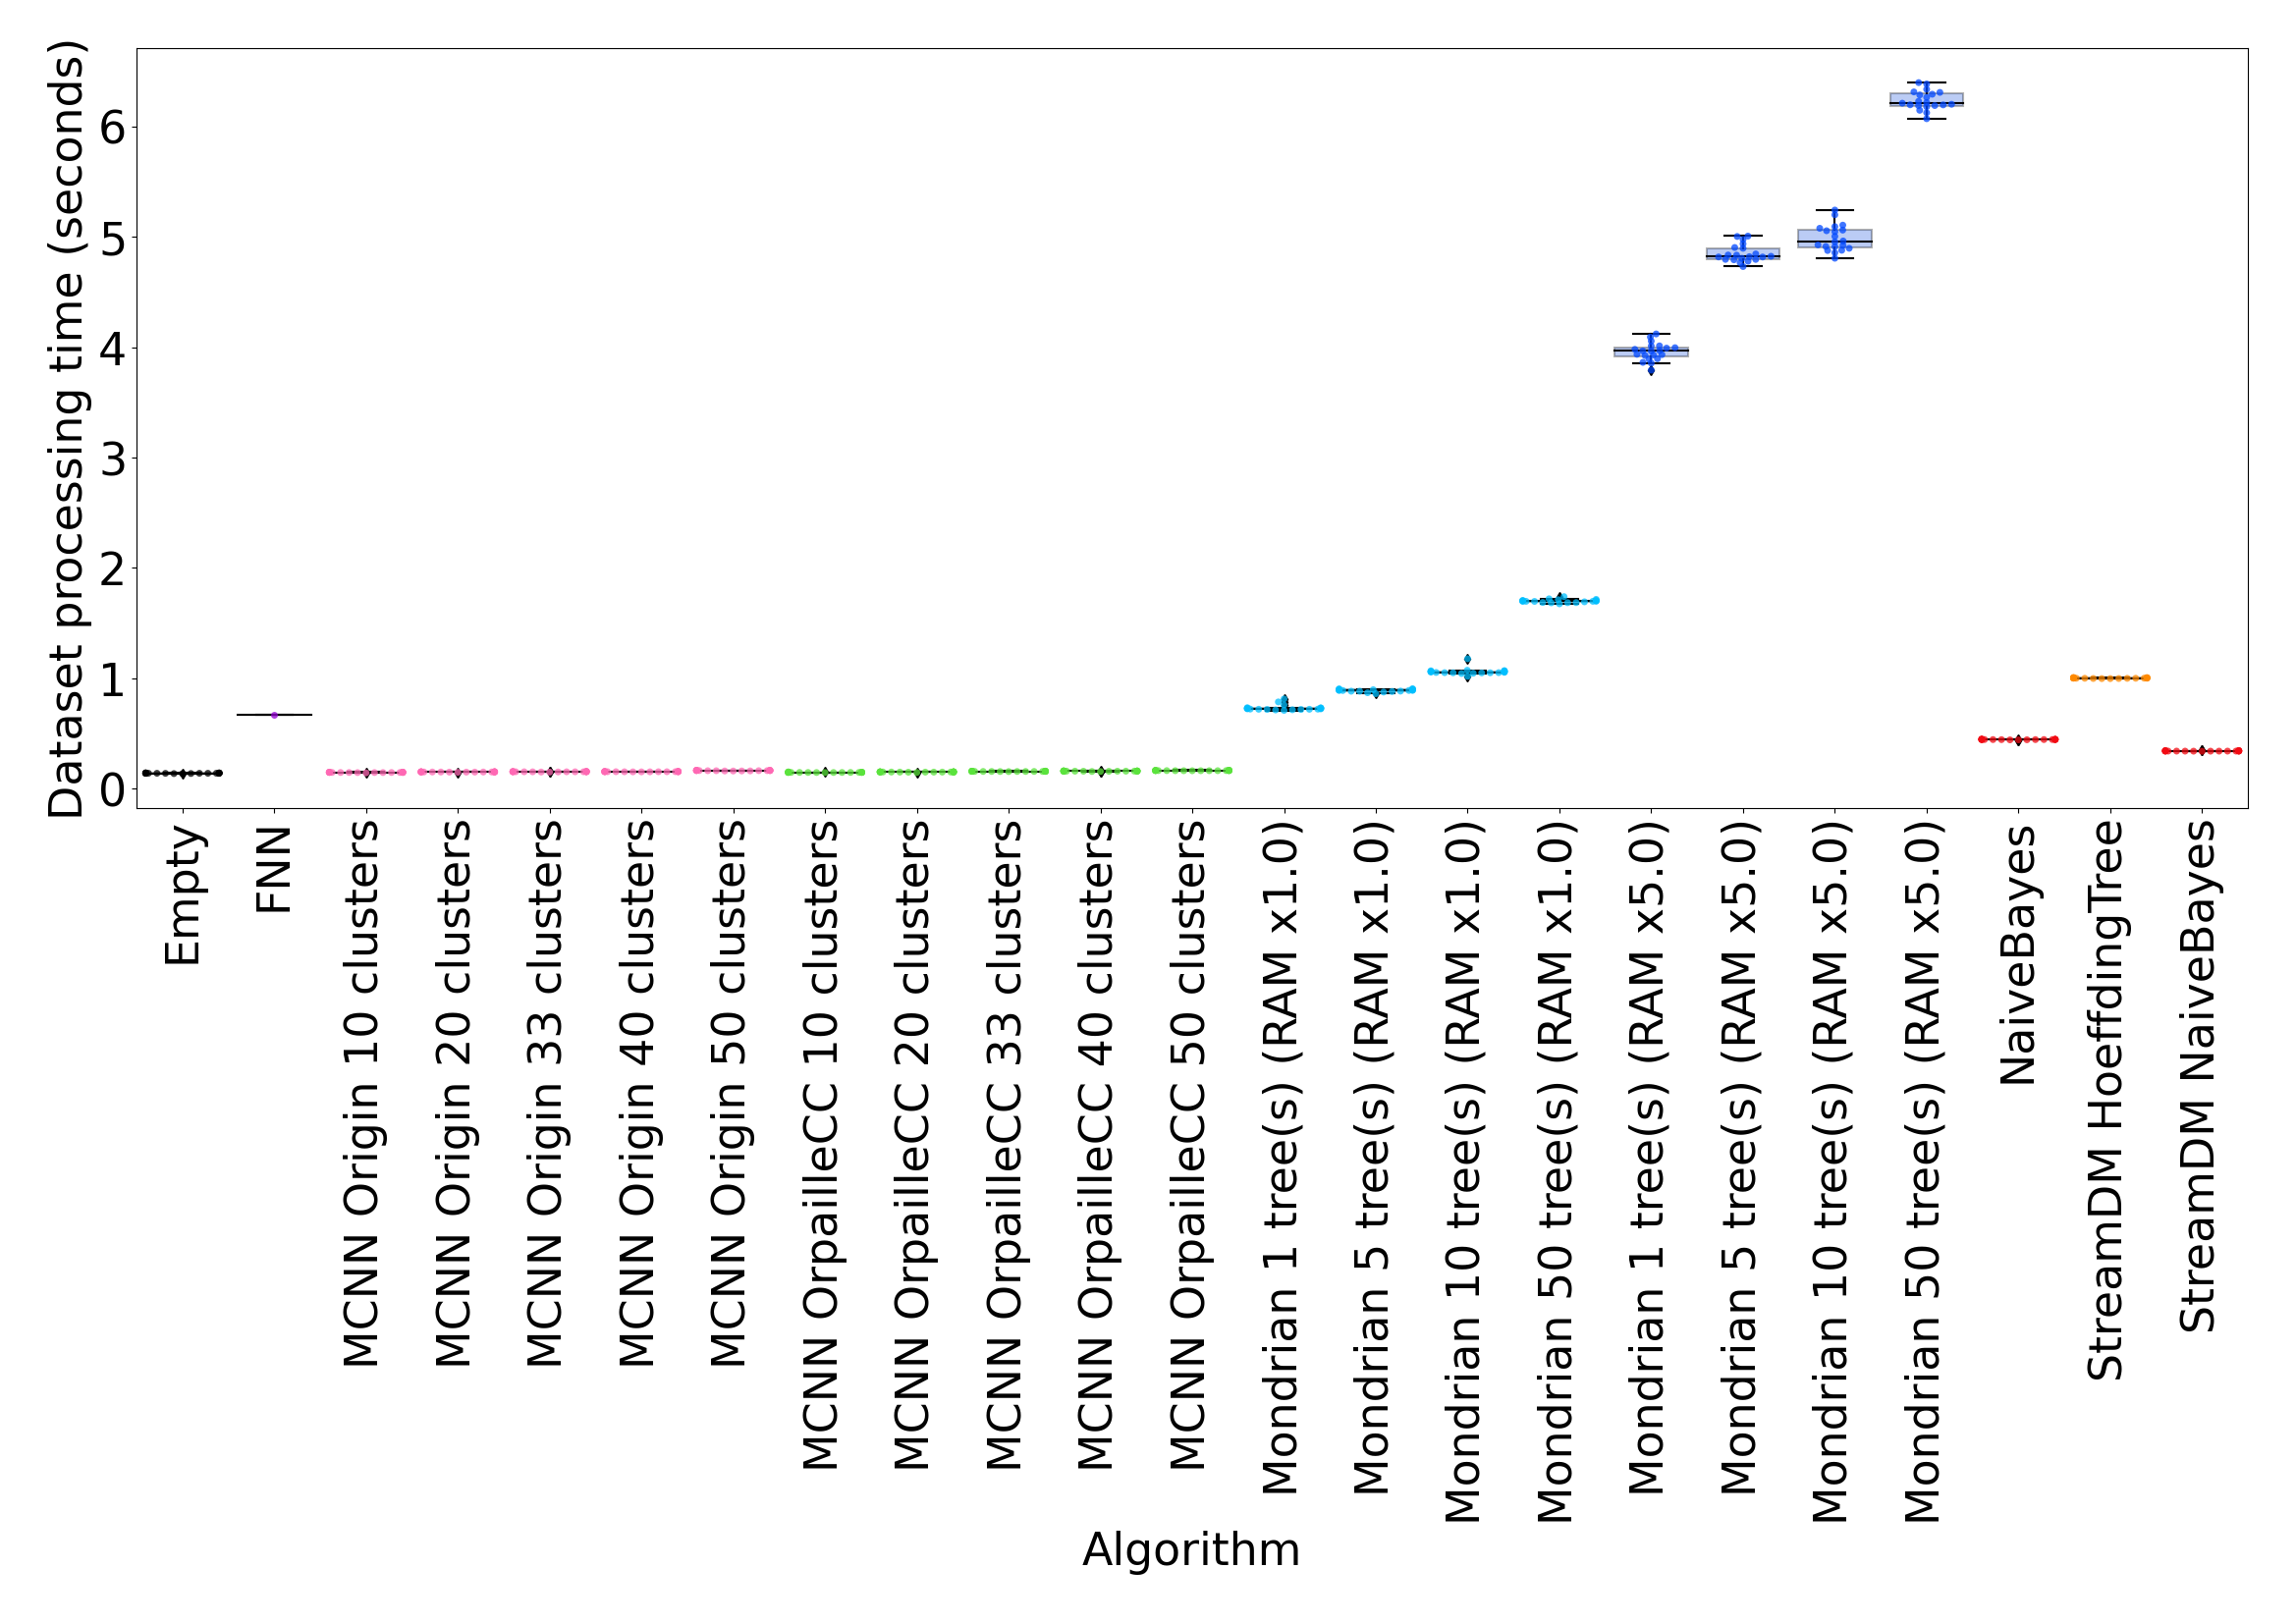
\includegraphics[width=\linewidth]{figures/results/banos_6_runtime.png}
		\caption{\banosdataset}
		\label{fig:runtime-banos}
	\end{subfigure}
	\hfill
	\begin{subfigure}[t]{.49\linewidth}
		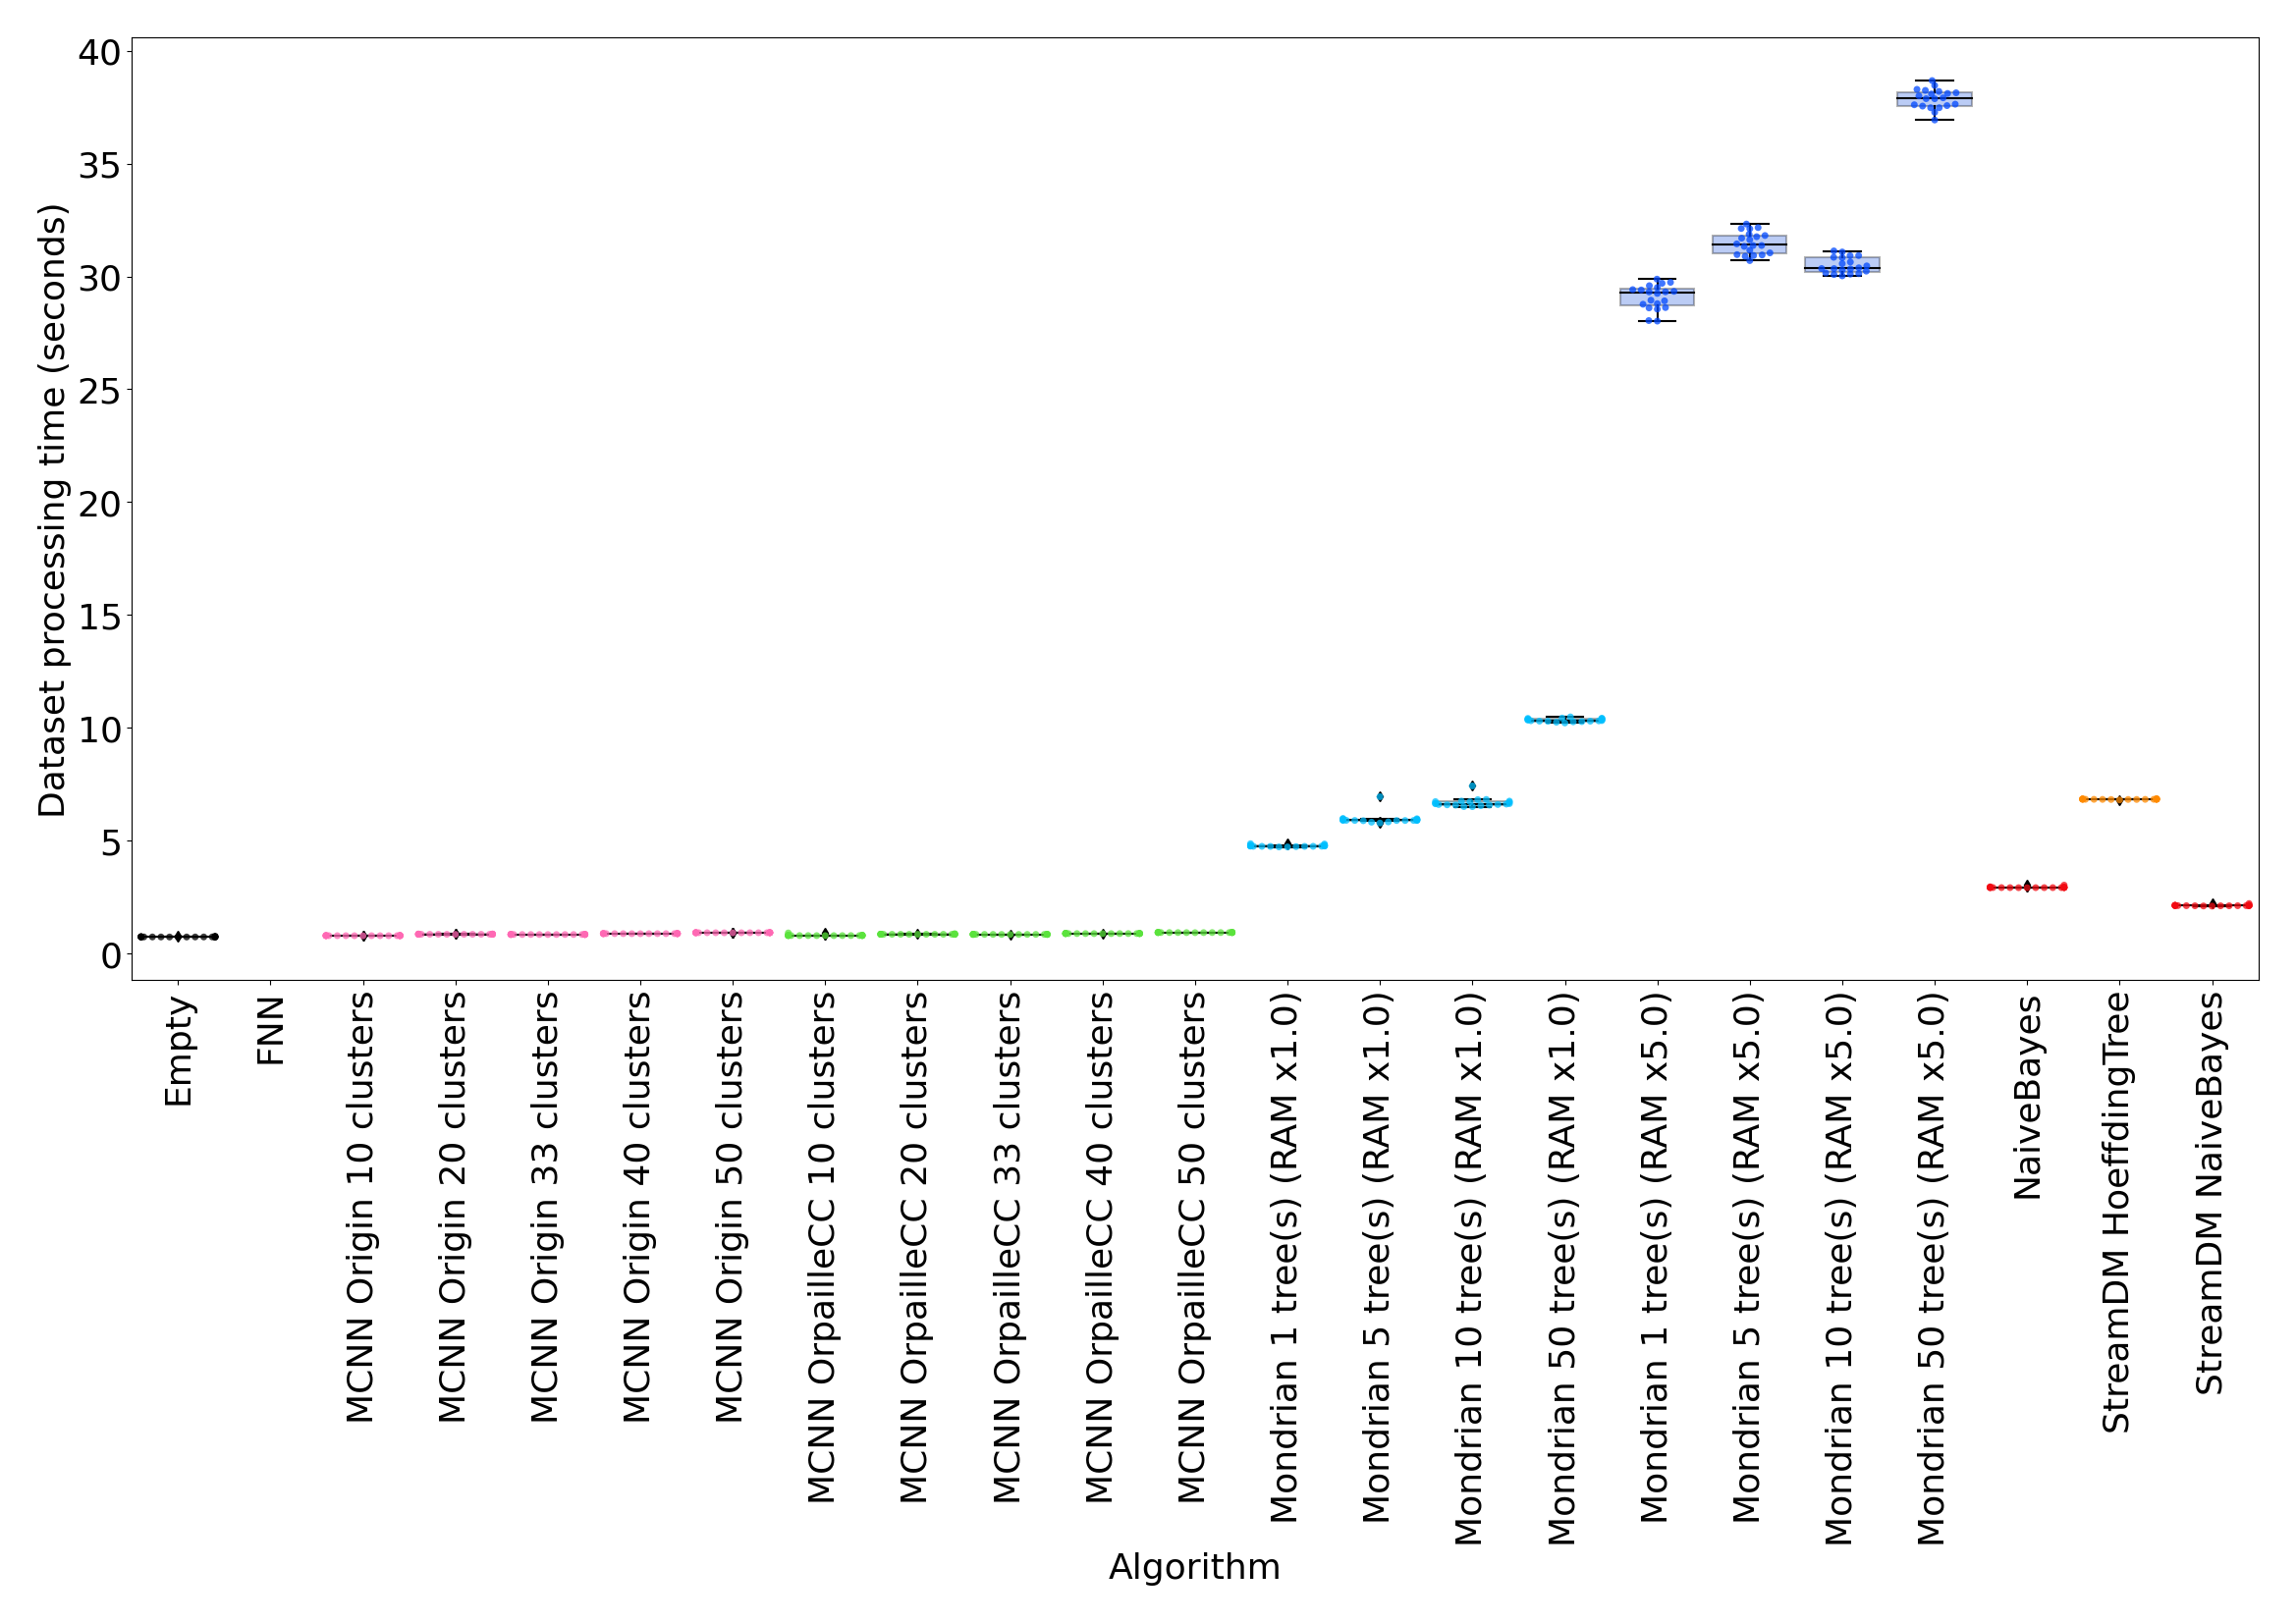
\includegraphics[width=\linewidth]{figures/results/recofit_6_runtime.png}
		\caption{\recofitdataset}
		\label{fig:runtime-recofit}
	\end{subfigure}
	\caption{Runtime with the two real datasets (20 repetitions).}
	\label{fig:runtime}
\end{figure*}

\subsection{Memory}
\label{sec:result-memory}
Figure~\ref{fig:memory} shows the evolution of the memory footprint for the
\banosdataset dataset. Because we focus on the classifiers footprint, the
figure only shows the memory difference between the classifiers and an empty
classifier. 

Memory footprint is similar across all datasets, due to the fact that most
algorithms follow a bounded memory policy or have a constant space complexity.
The only exception is the \hoeffdingtree that constantly selects new splits
depending on new data points. The \mondrianforest have the same behavior but
OrpailleCC implementation include a memory bound which make its memory
footprint constant.
\TG{Last two sentences should be improved, this can be written in a more compact way.}.

\begin{figure}
	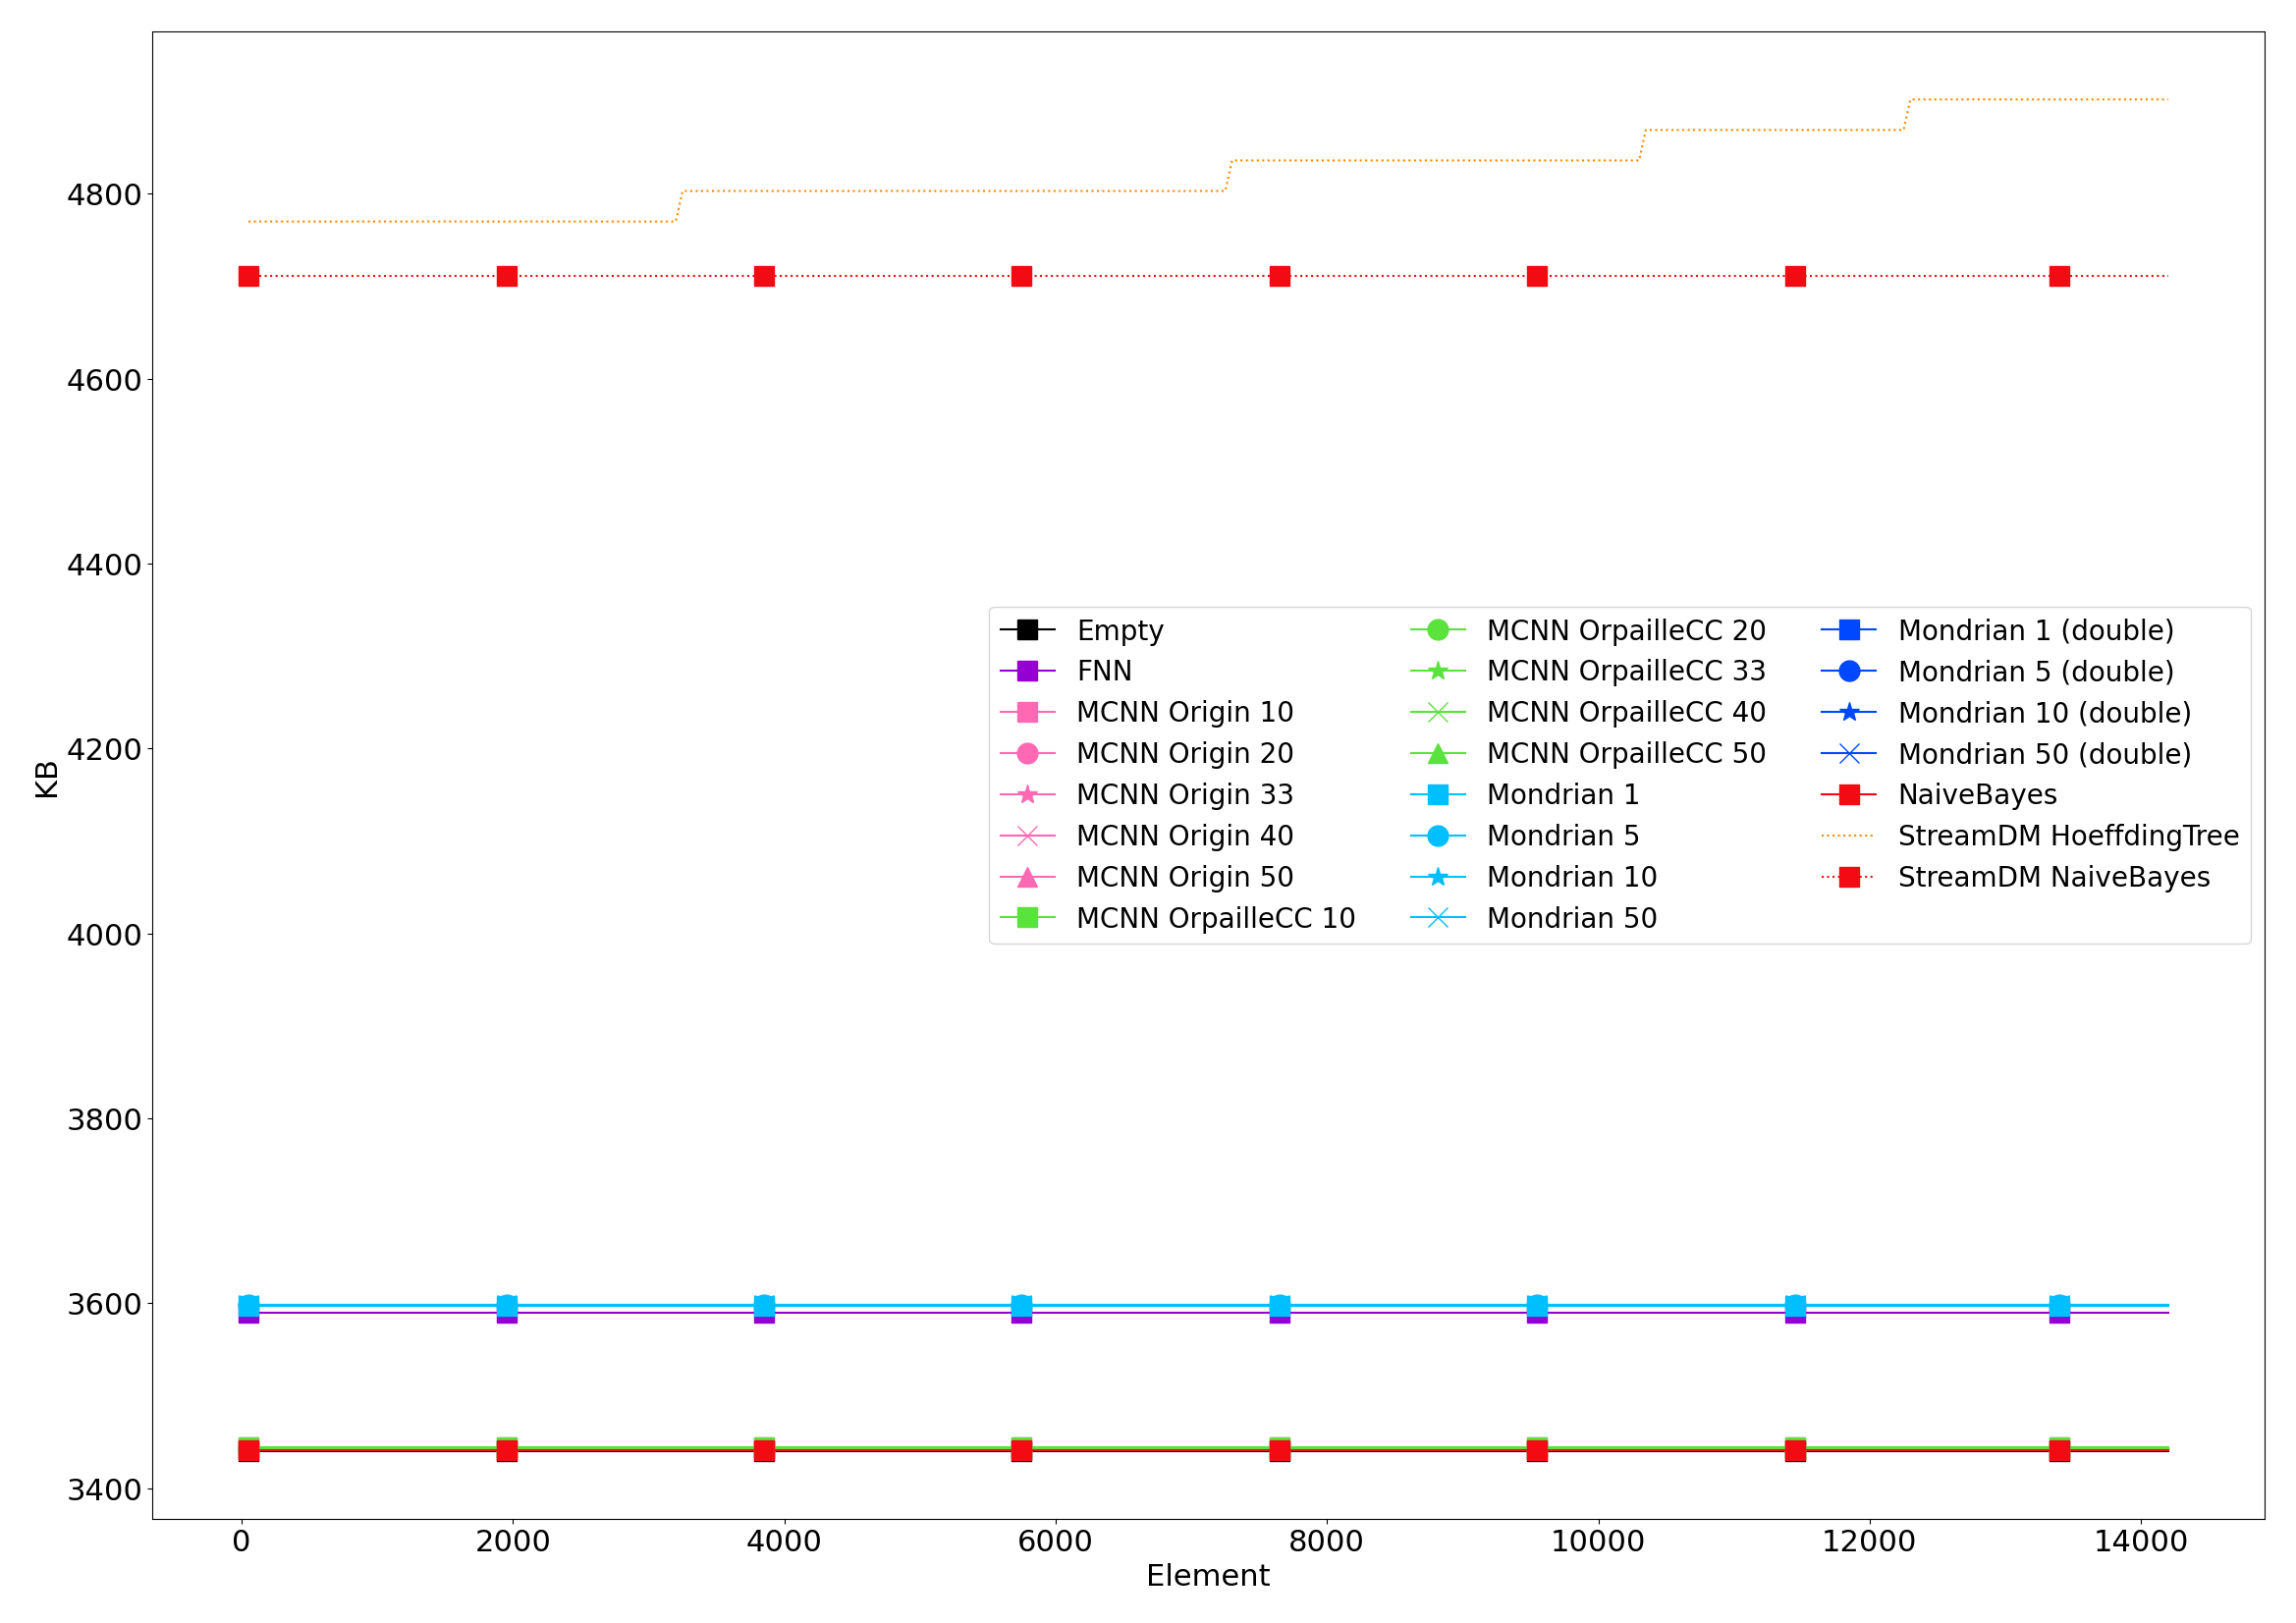
\includegraphics[width=\linewidth]{figures/results/banos_3_memory.png}
	\caption{Memory footprint of the classifiers compared to an empty
	classifier on the Banos dataset. The memory footprint of the empty
	classifier is slightly above 3.4~MB.\TG{increase font size in all graphs,
	to make it only slightly smaller than font size in caption}}
	\label{fig:memory}
\end{figure}


\subsection{Micro-Cluster Nearest Neighbor Hyperparameters}

Figure~\ref{fig:mcnn-tuning-error} shows the impact of the error threshold
in the \mcnn classifiers with different cluster count. The error
threshold of \mcnn has little impact on the classification performance. For
20 and 40 clusters, the best-performing threshold is either 2 or 4, meaning
that a cluster may do 2 or 4 errors before being split. For 10 clusters,
all error thresholds perform equally.

\begin{figure}
	 \begin{subfigure}[b]{0.49\textwidth}
		 \centering
		 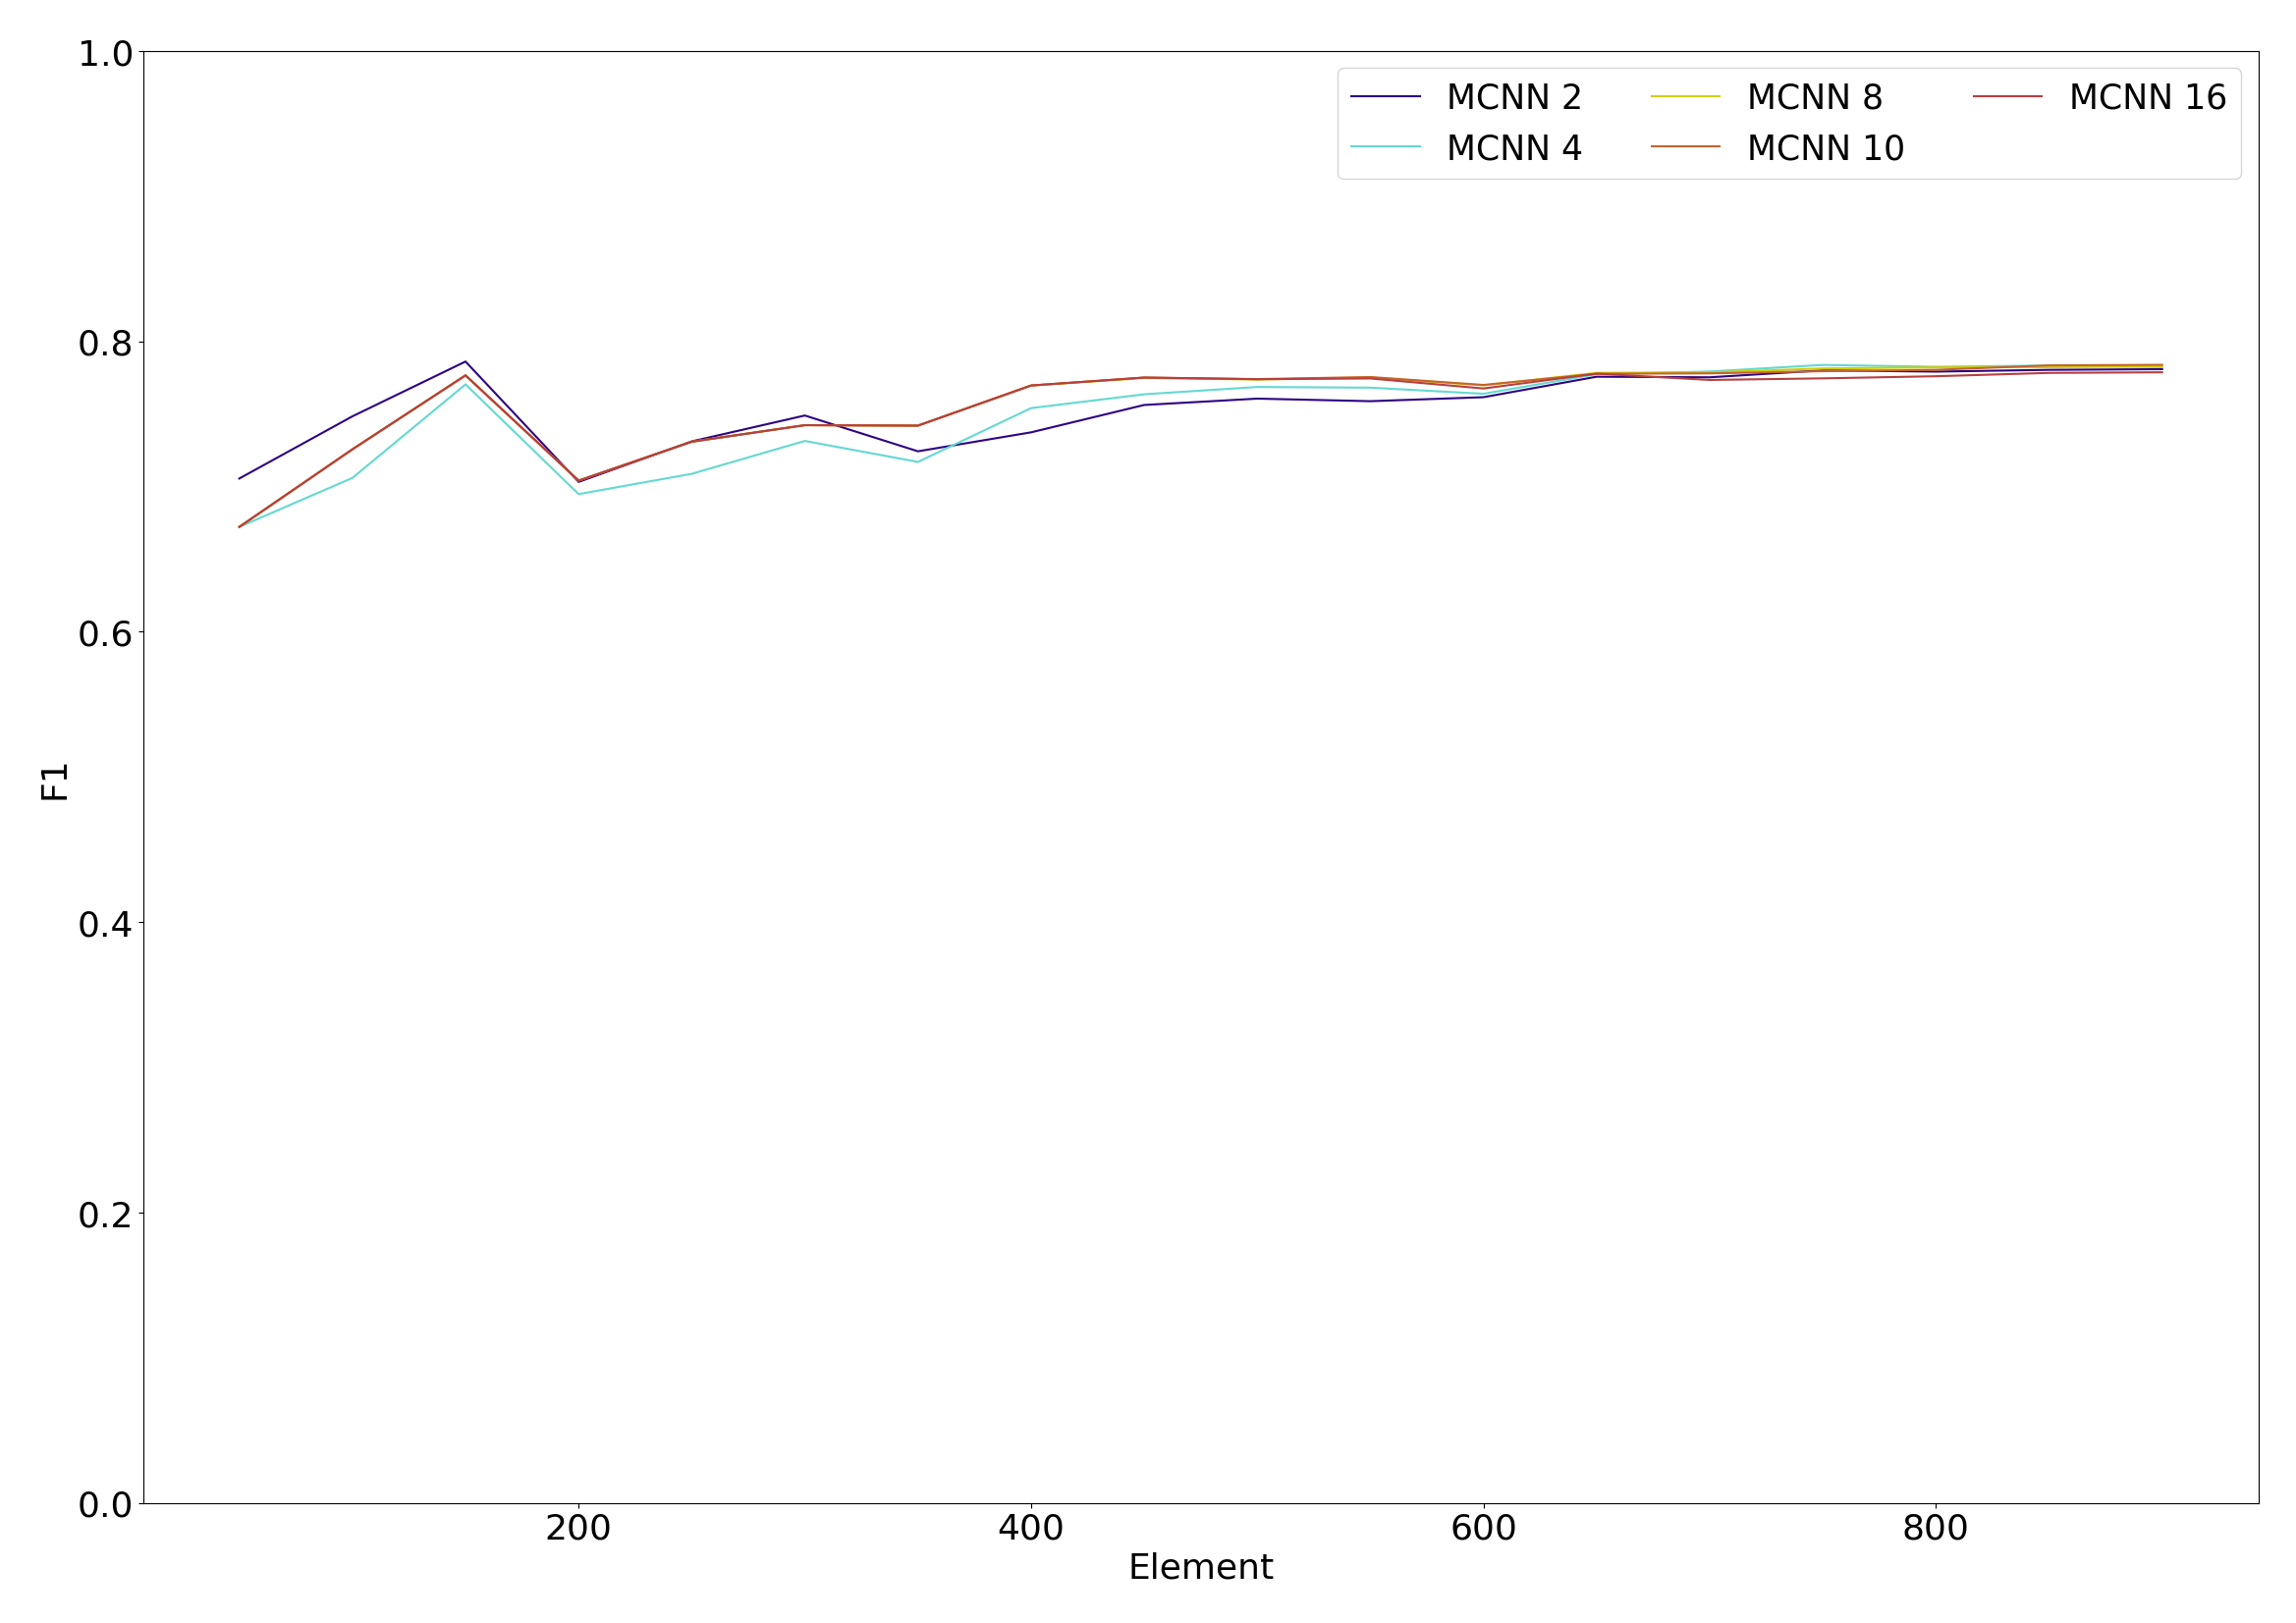
\includegraphics[width=\linewidth]{figures/calibration_mcnn_40.png}
		 \caption{40 clusters}
	 \end{subfigure}
	 \begin{subfigure}[b]{0.49\textwidth}
		 \centering
		 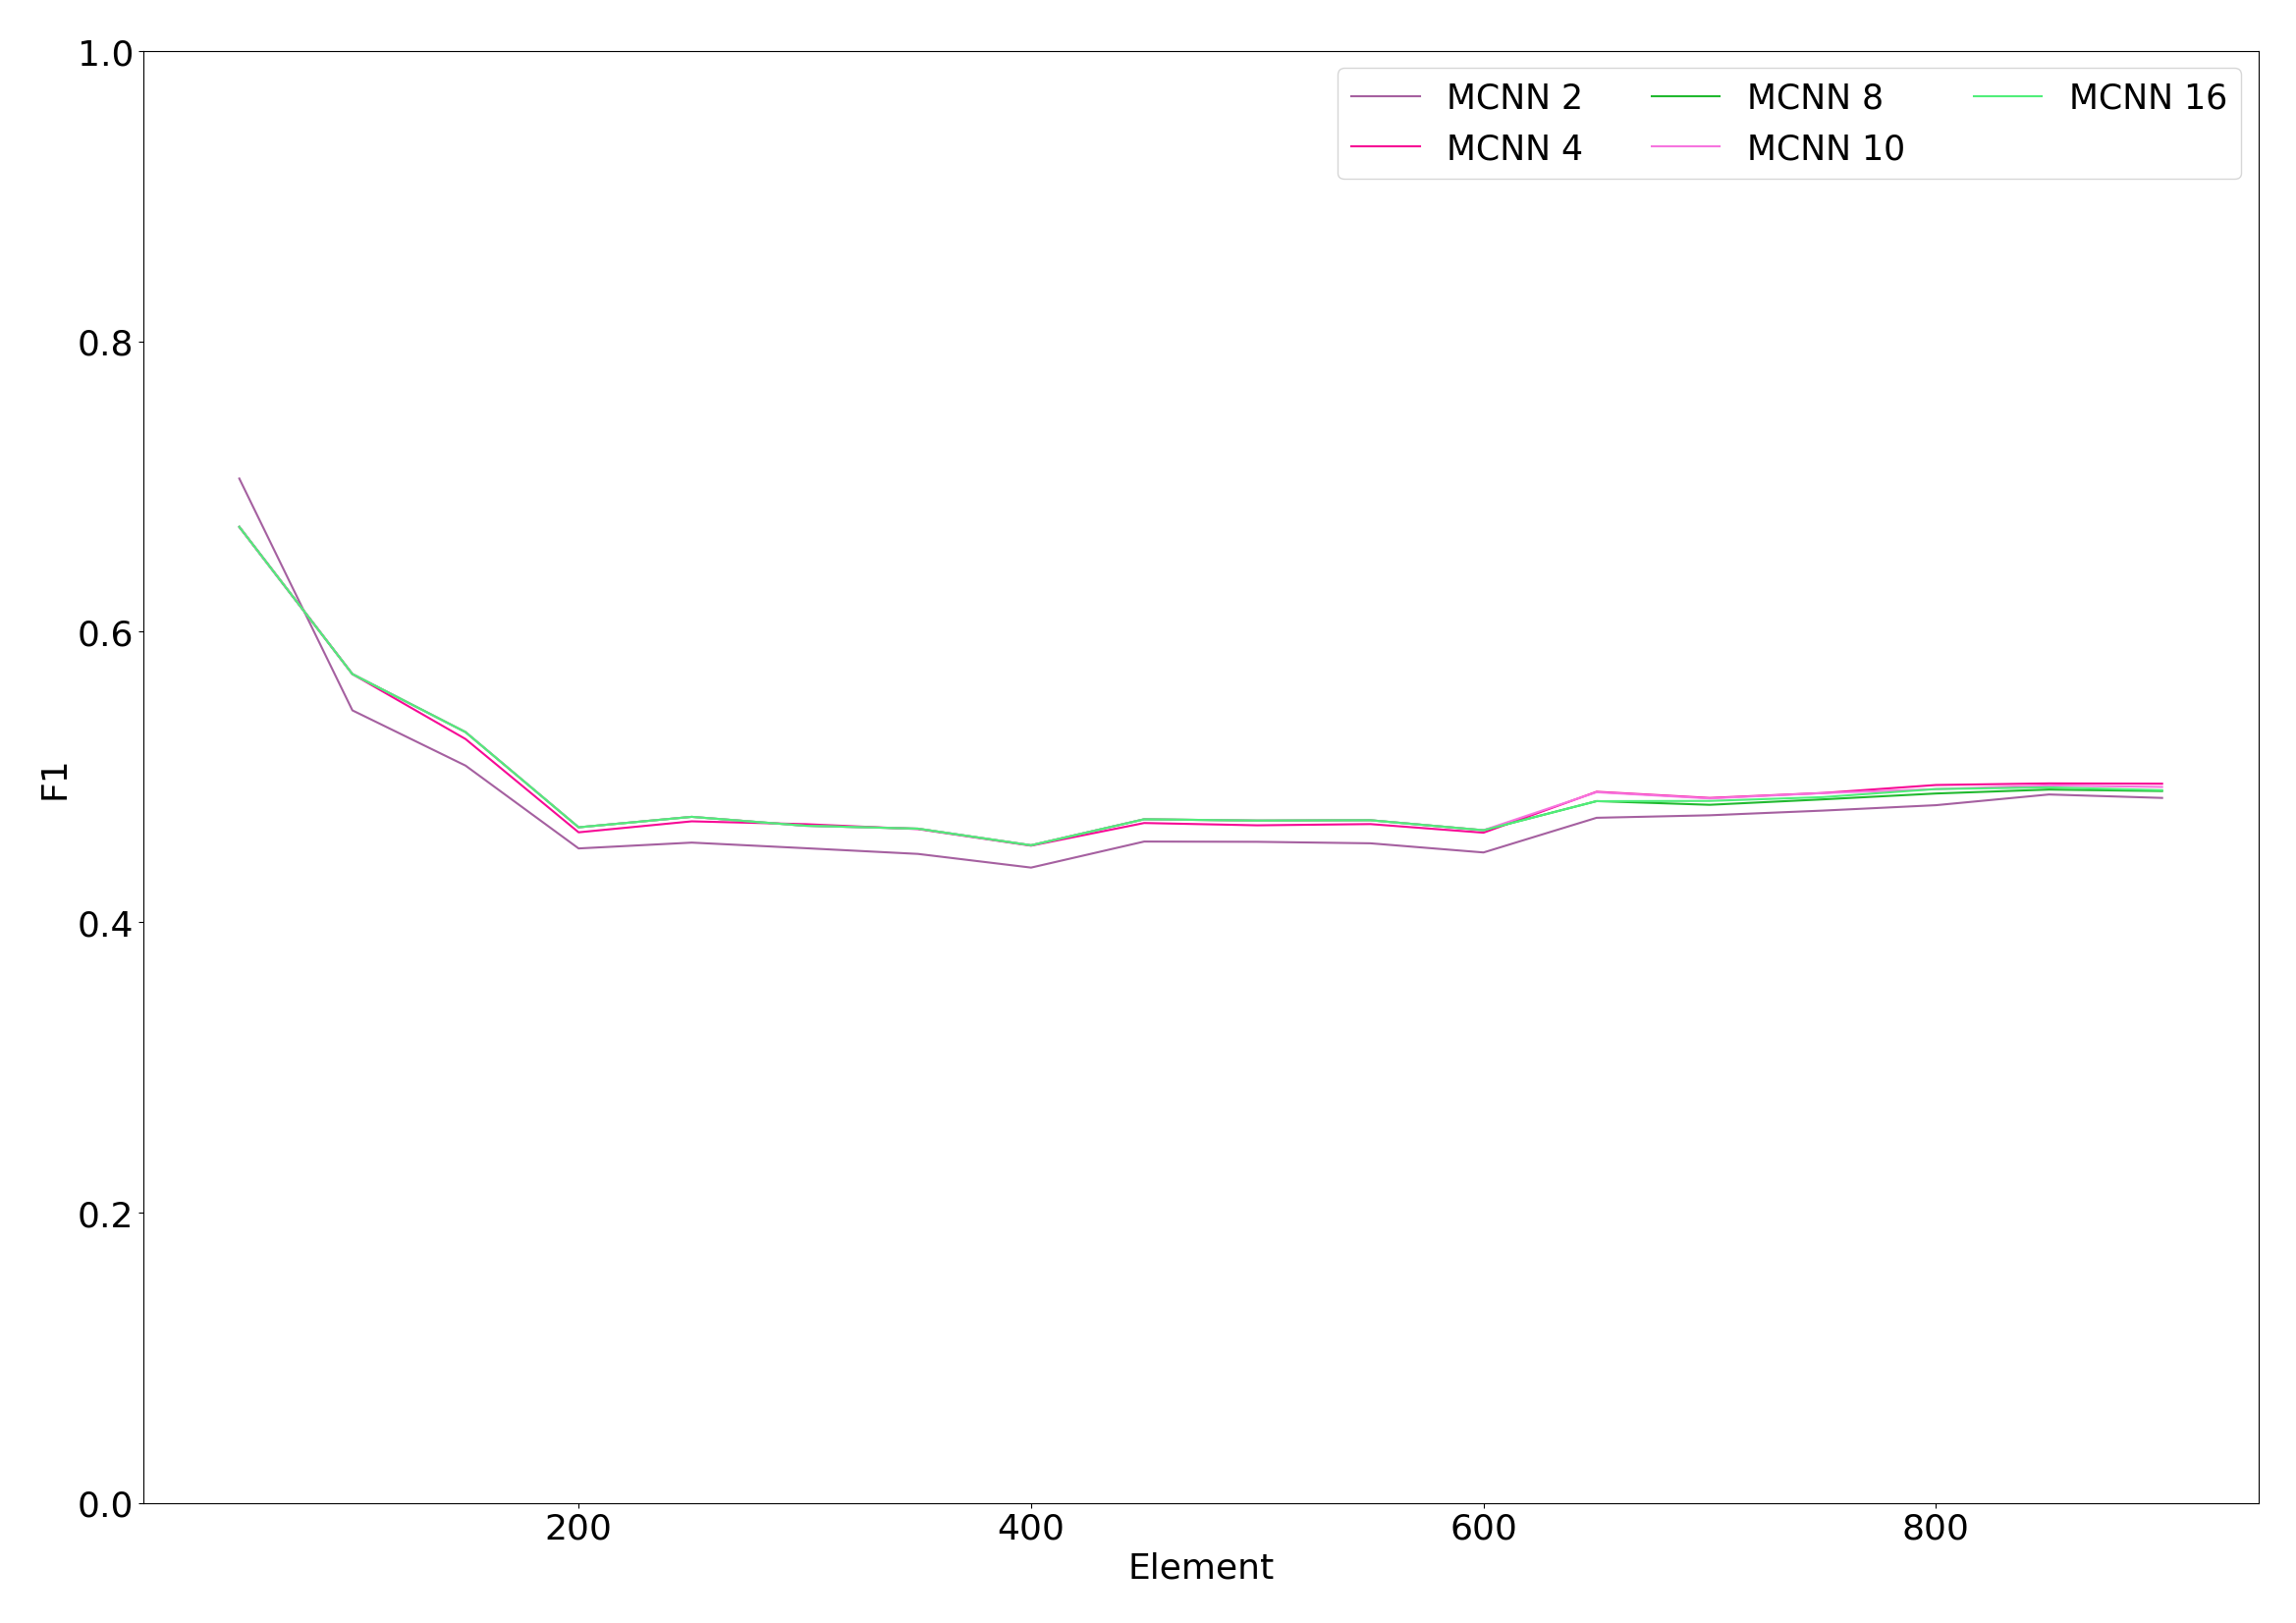
\includegraphics[width=\linewidth]{figures/calibration_mcnn_20.png}
		 \caption{20 clusters}
	 \end{subfigure}
	 \begin{subfigure}[b]{0.49\textwidth}
		 \centering
		 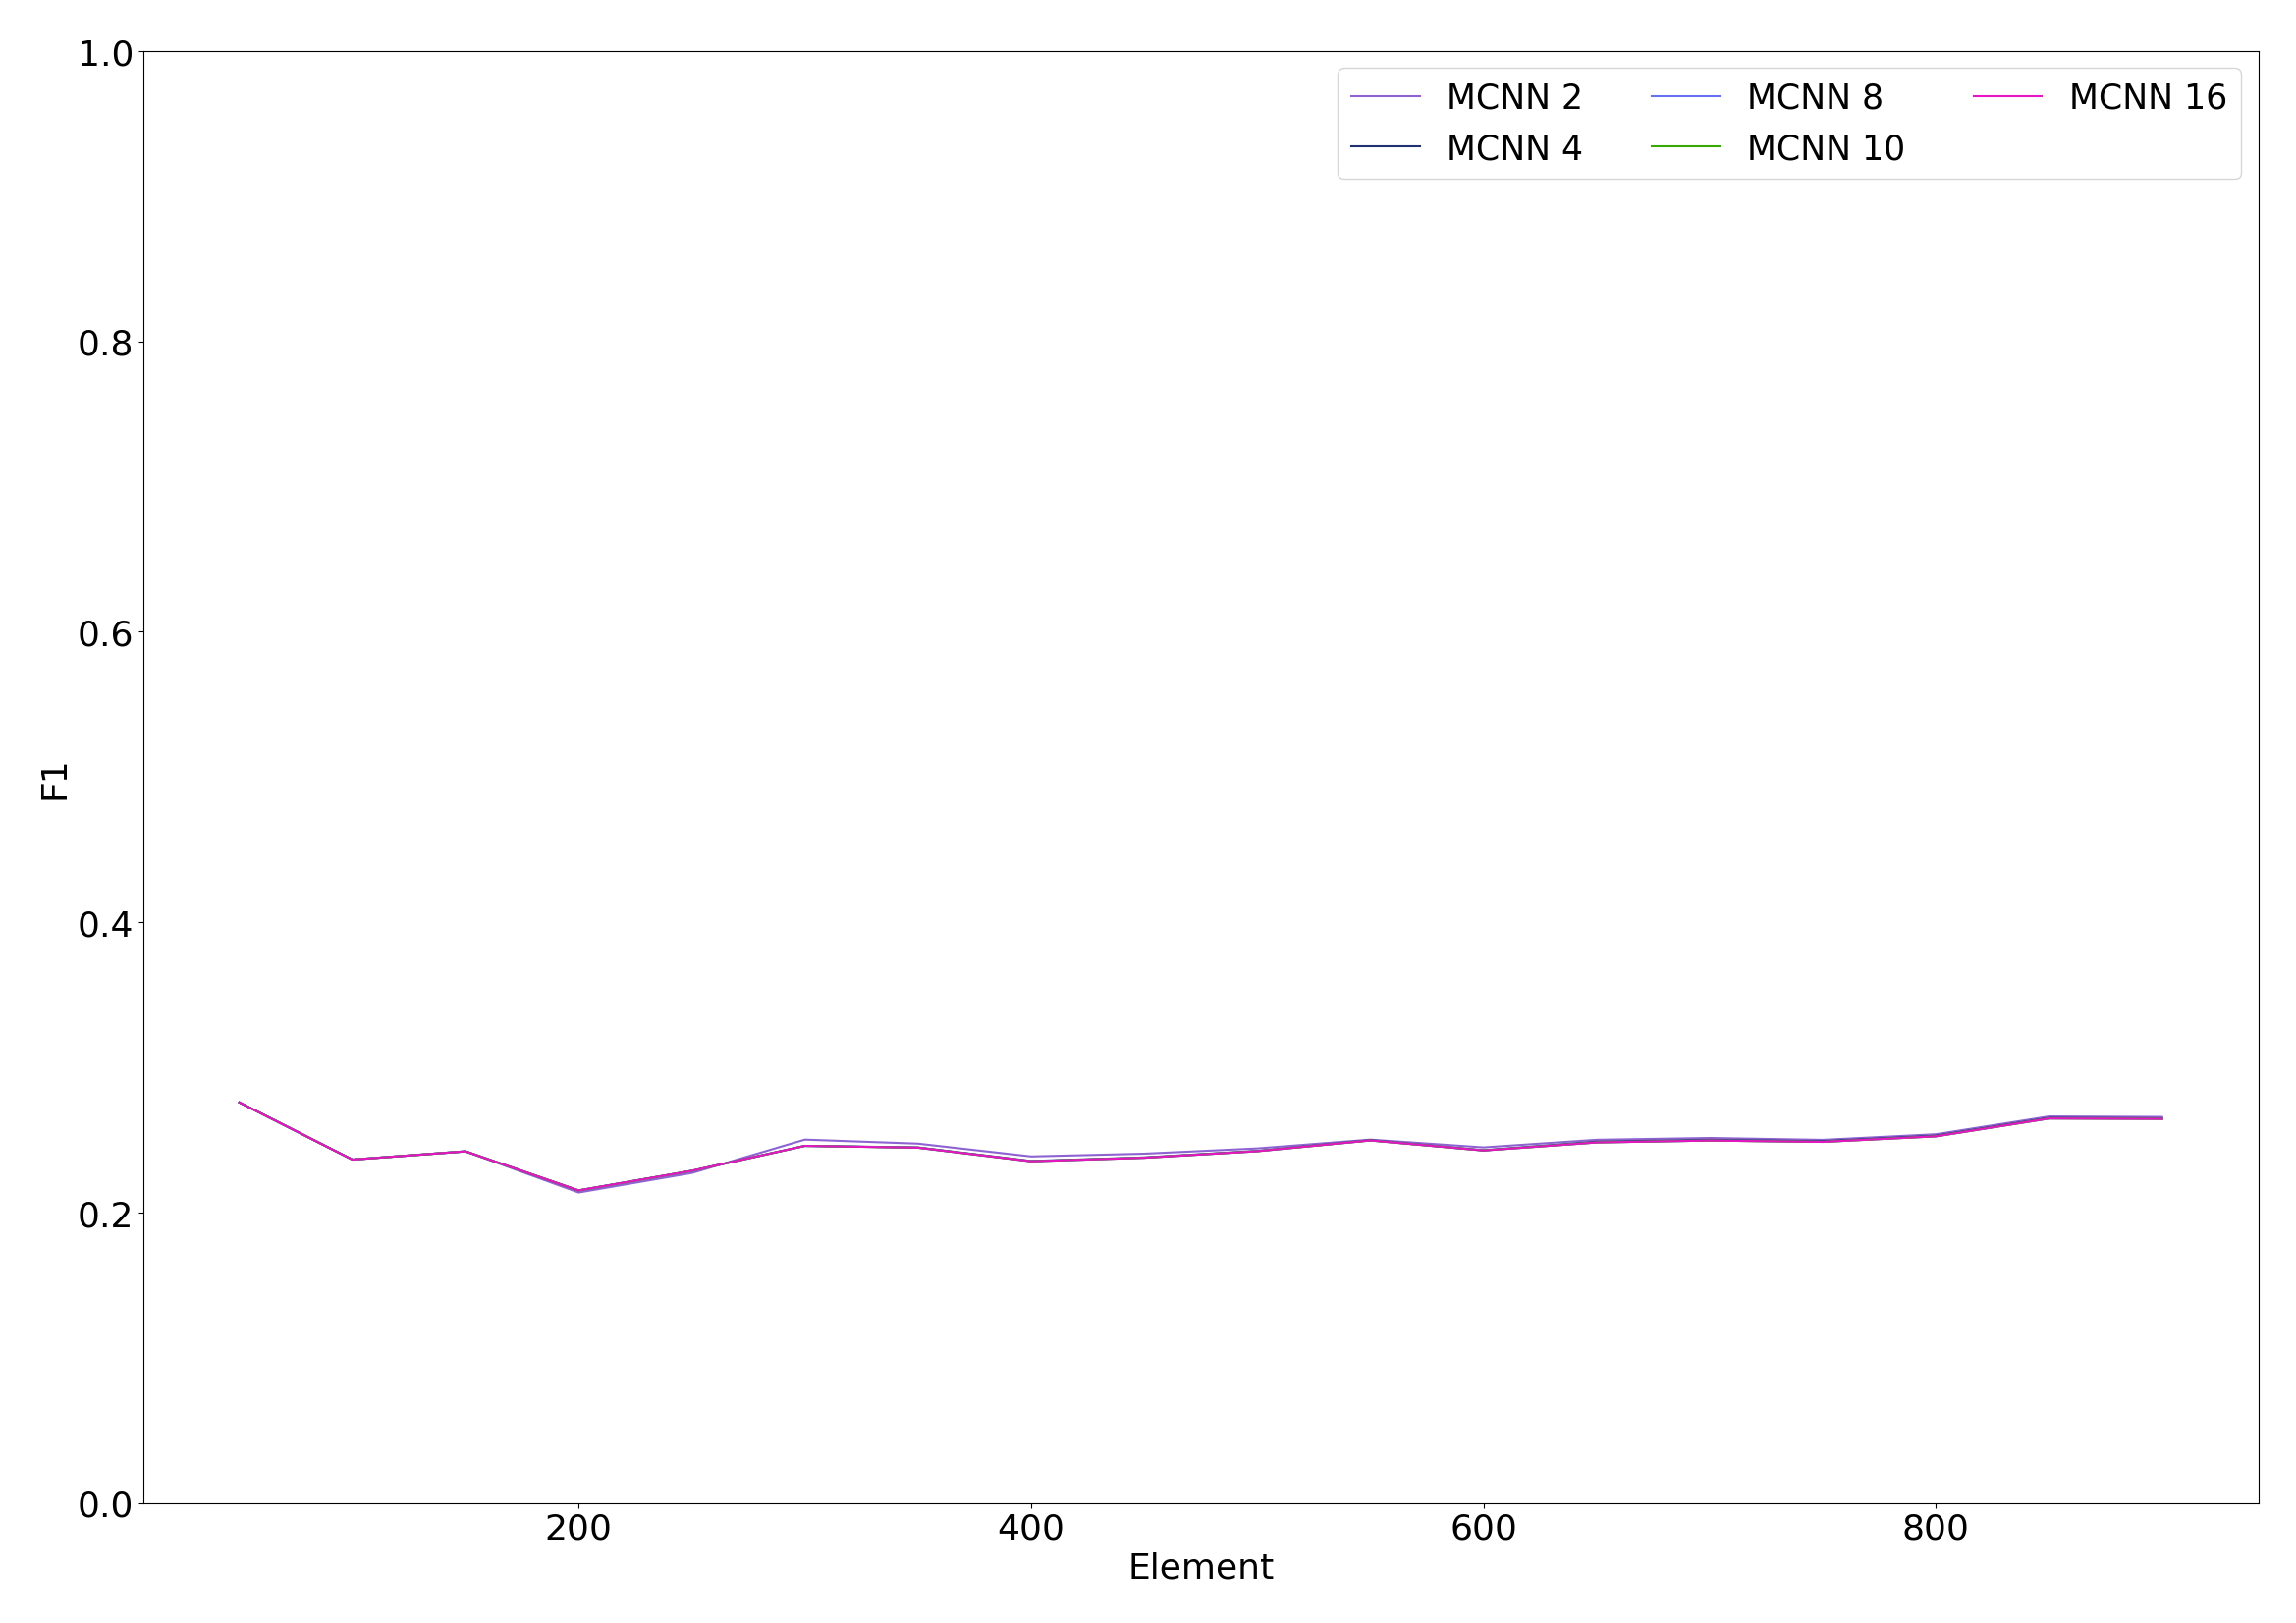
\includegraphics[width=\linewidth]{figures/calibration_mcnn_10.png}
		 \caption{10 clusters}
	 \end{subfigure}
	\caption{Hyperparameters tuning of \mcnn with first subject of \banosdataset dataset. \TG{It's a bit weird to use accuracy here while F1 score was used before. 
	Couldn't you just use F1 score here too?}}
	\label{fig:mcnn-tuning-error}
\end{figure}

\subsection{\mondrianforest Hyperparameters}

Figure~\ref{fig:mondrian-tuning} shows the impact of the \mondrianforest hyperparameters on
the classification performance. Occasionally, dashed lines are used to
emphasize the minimum and the maximum \TG{That's a comment for the caption. Why ``occasionally'' and not always?}.

The base count hyperparameter (Figure~\ref{fig:mondrian-base-count}) has a
very substantial impact on classification performance; the smallest value
(0.005) results in the best performance. On the contrary, the
budget hyperparameter (Figure~\ref{fig:mondrian-budget}) only has a
moderate impact on classification; the best value is slightly below
1.0. Finally, the discount hyperparameter
(Figure~\ref{fig:mondrian-discount}) has a negligible impact on the
performance; the best-performing value is 0.1.

\begin{figure}
	 \centering
	 \begin{subfigure}[b]{0.49\textwidth}
		\centering
		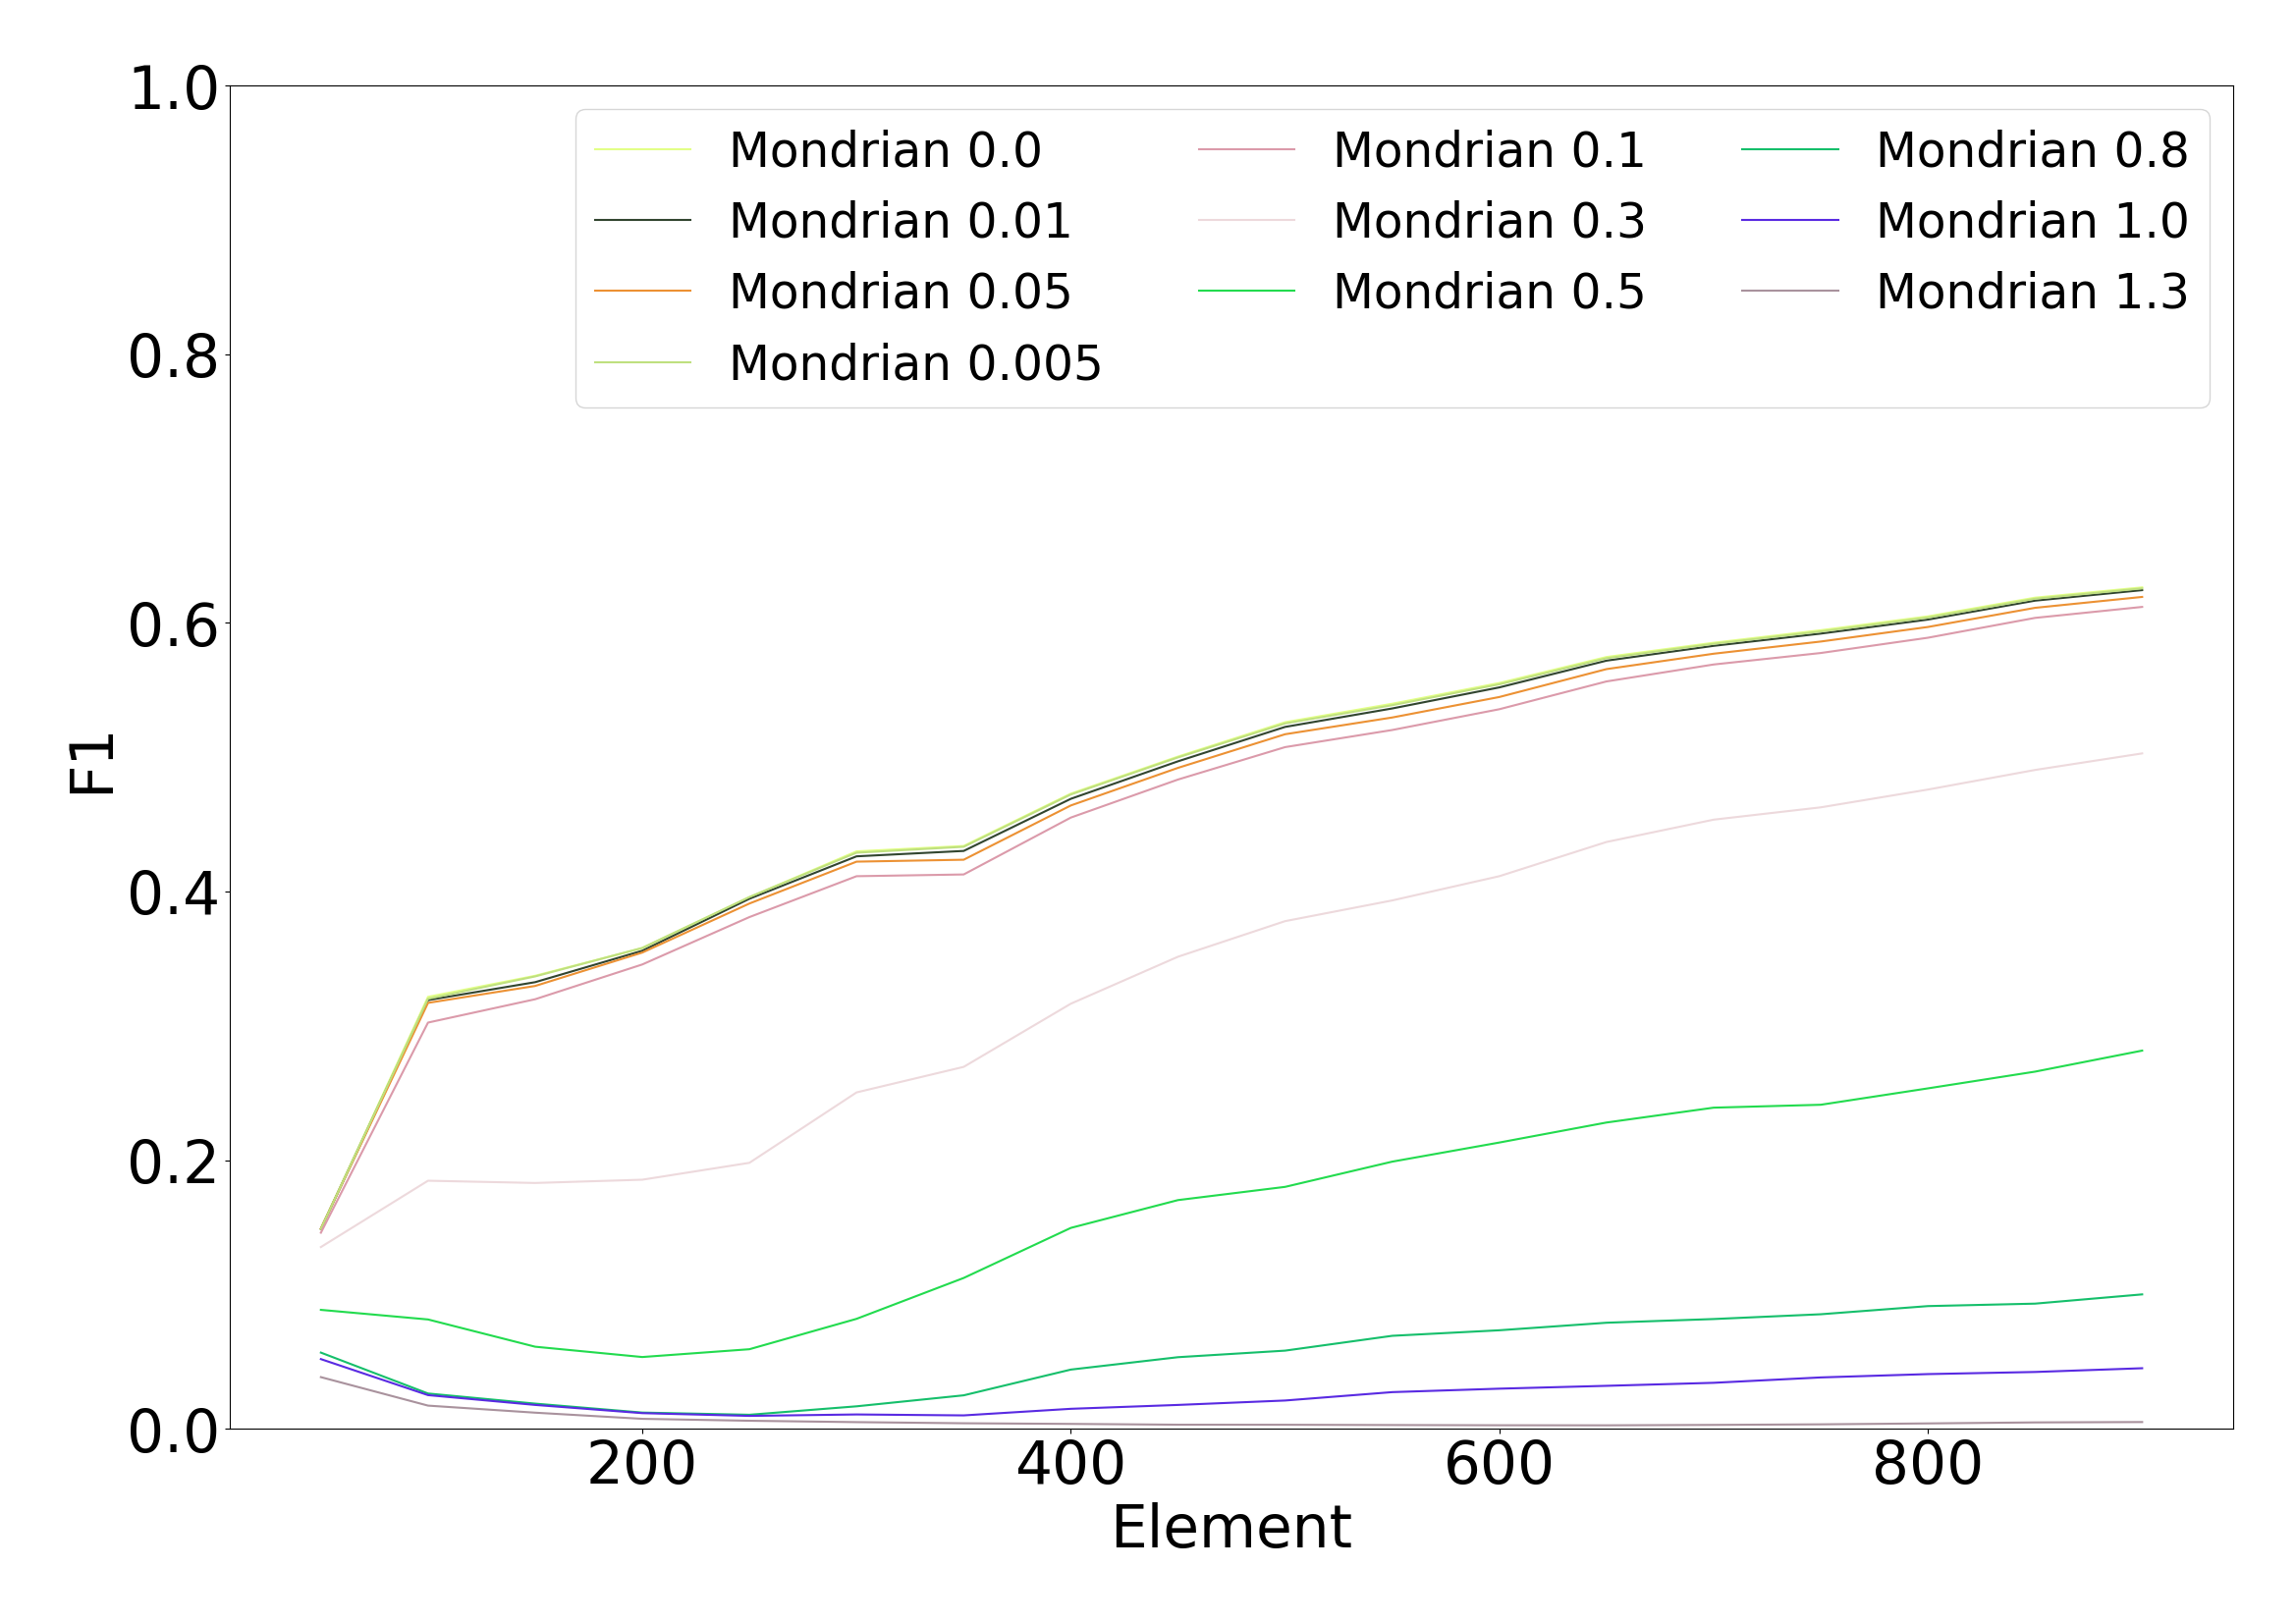
\includegraphics[width=\textwidth]{figures/calibration_mondrian_base.png}
		\caption{Impact of the base count with 10 trees, a budget of $1.0$, and a discount factor of $0.2$. \TG{Could you simplify the figure legend to just show ``Mondrian - <base count>''? 
		it's a bit difficult to read and all parameters are the same and reported in this caption. Same comment for the other sub-figures.}} 
		\label{fig:mondrian-base-count}
	\end{subfigure}
	\hfill
	 \begin{subfigure}[b]{0.49\textwidth}
		 \centering
		 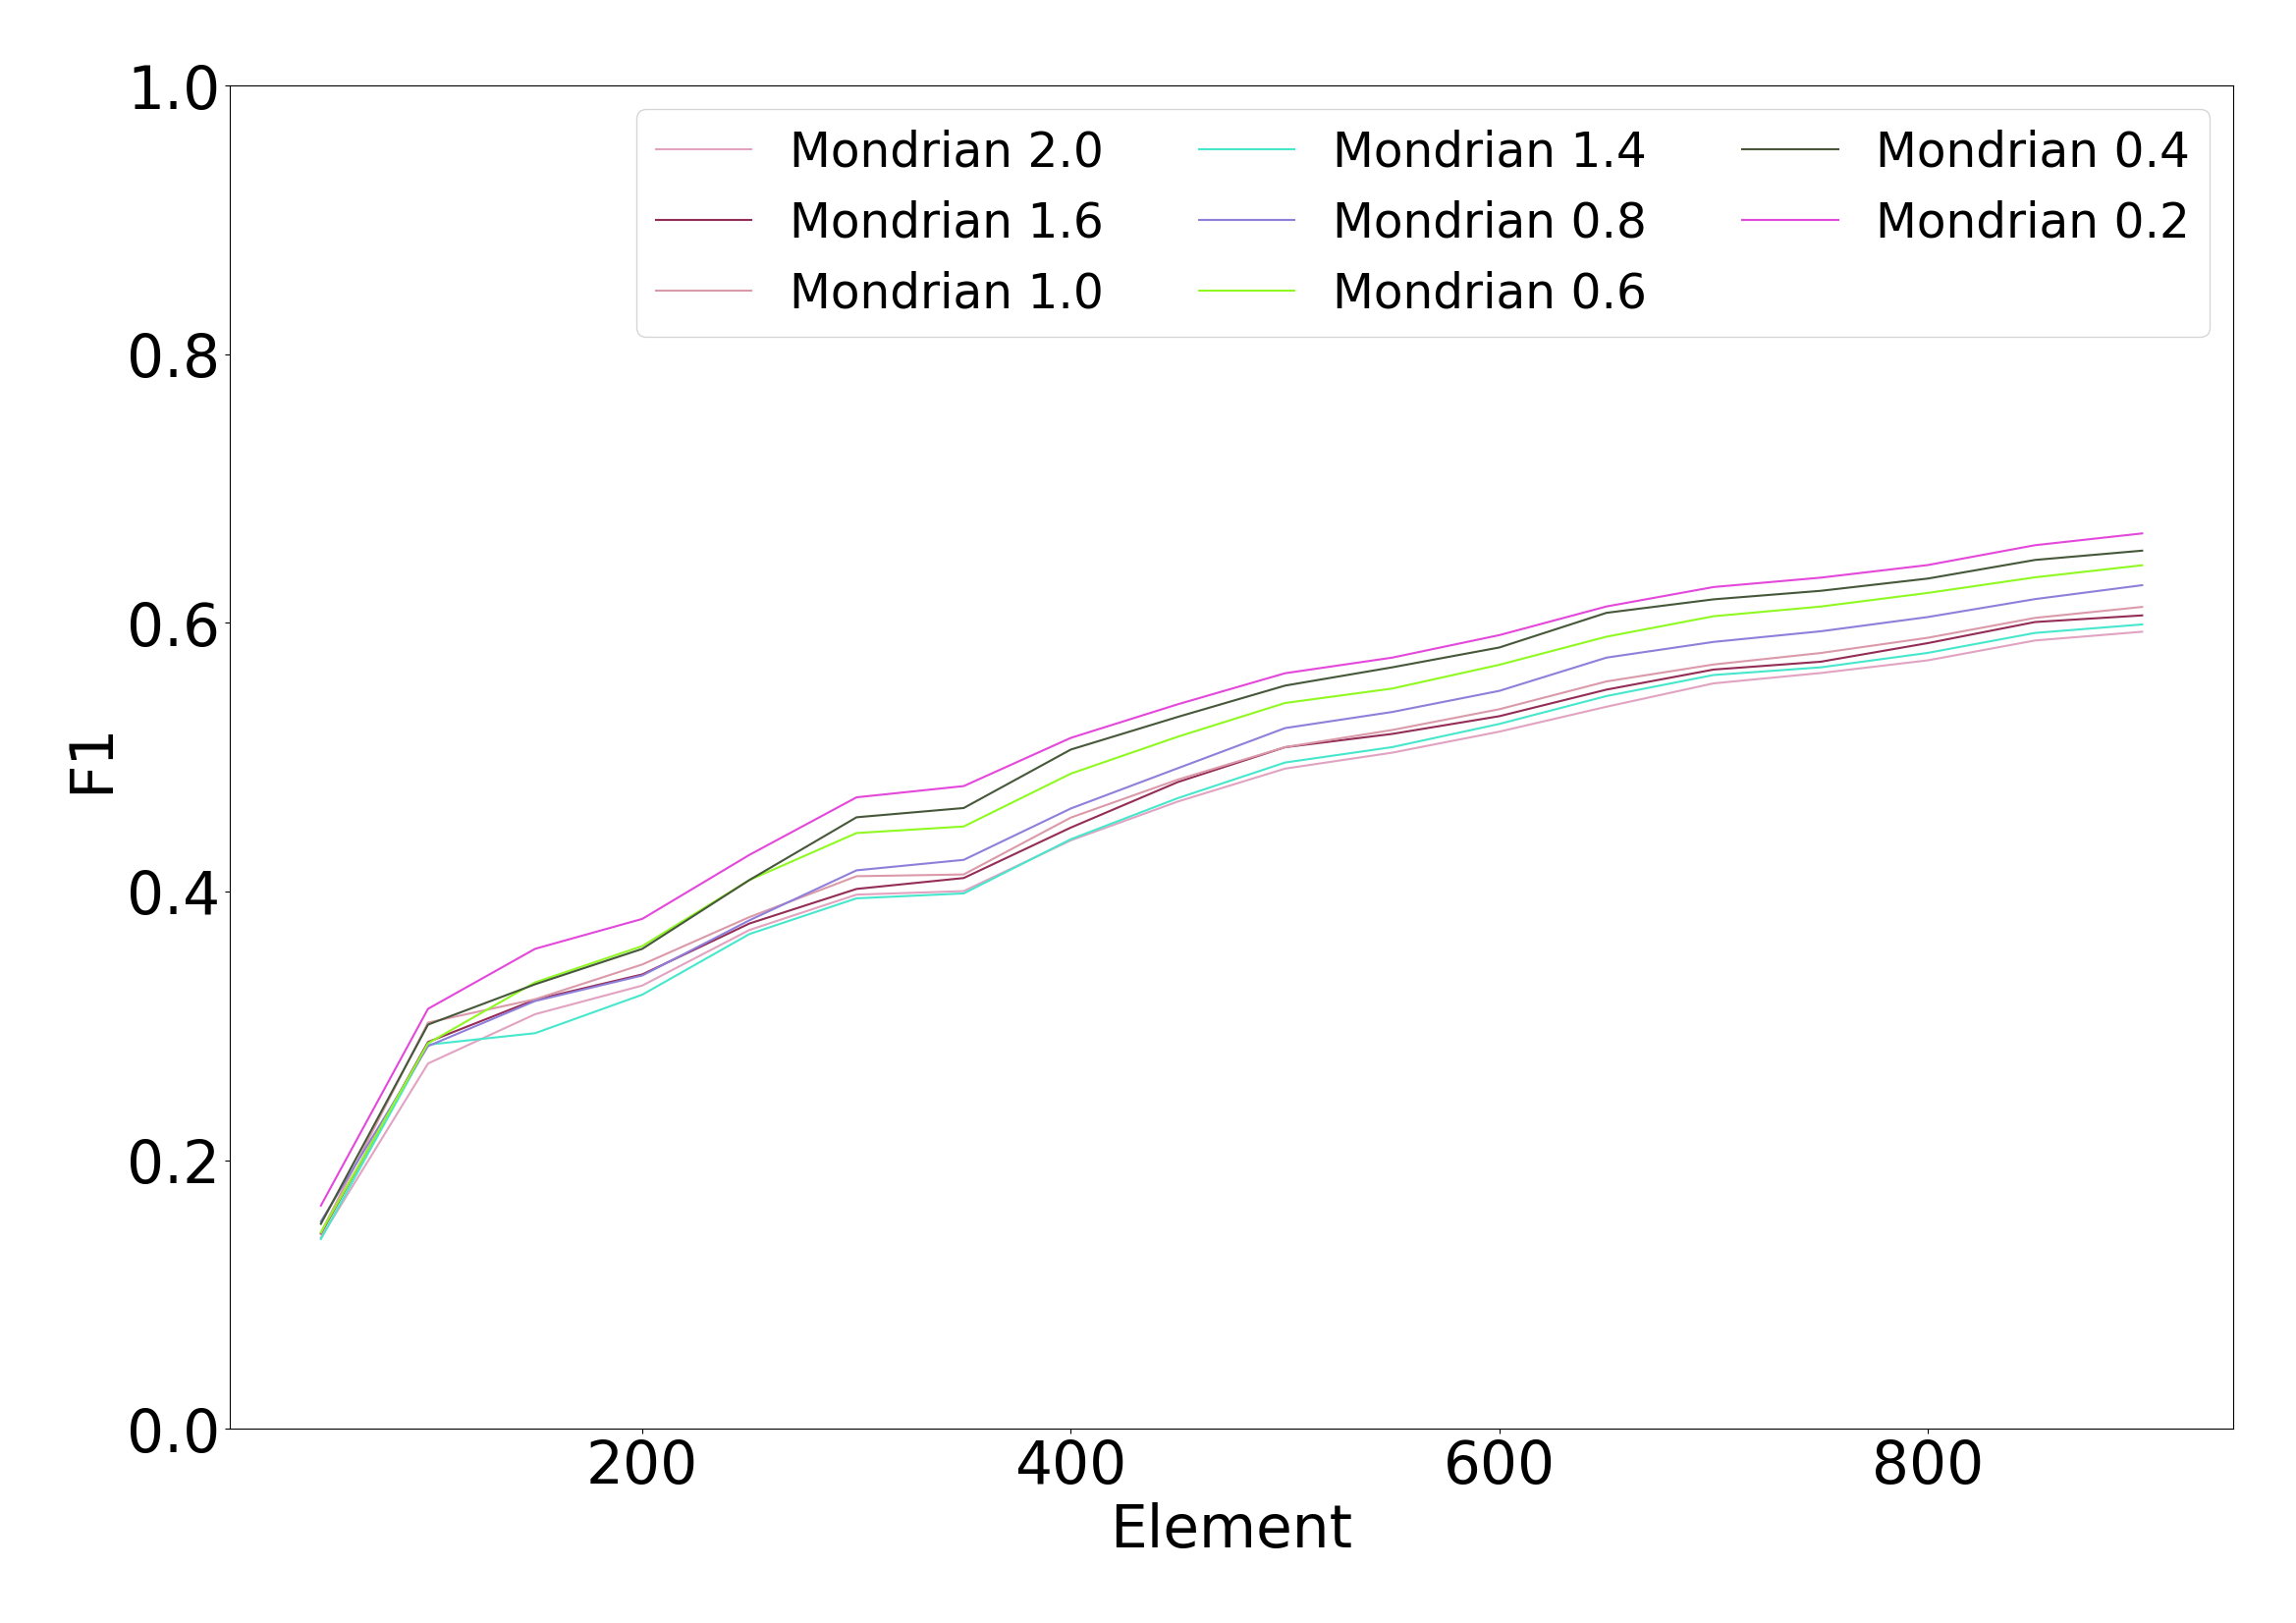
\includegraphics[width=\textwidth]{figures/calibration_mondrian_lifetime.png}
		 \caption{Impact of the budget with 10 trees, a base count of $0.1$, and discount factor of $0.2$.}
		 \label{fig:mondrian-budget}
	 \end{subfigure}
	 \hfill
	 \begin{subfigure}[b]{0.49\textwidth}
		 \centering
		 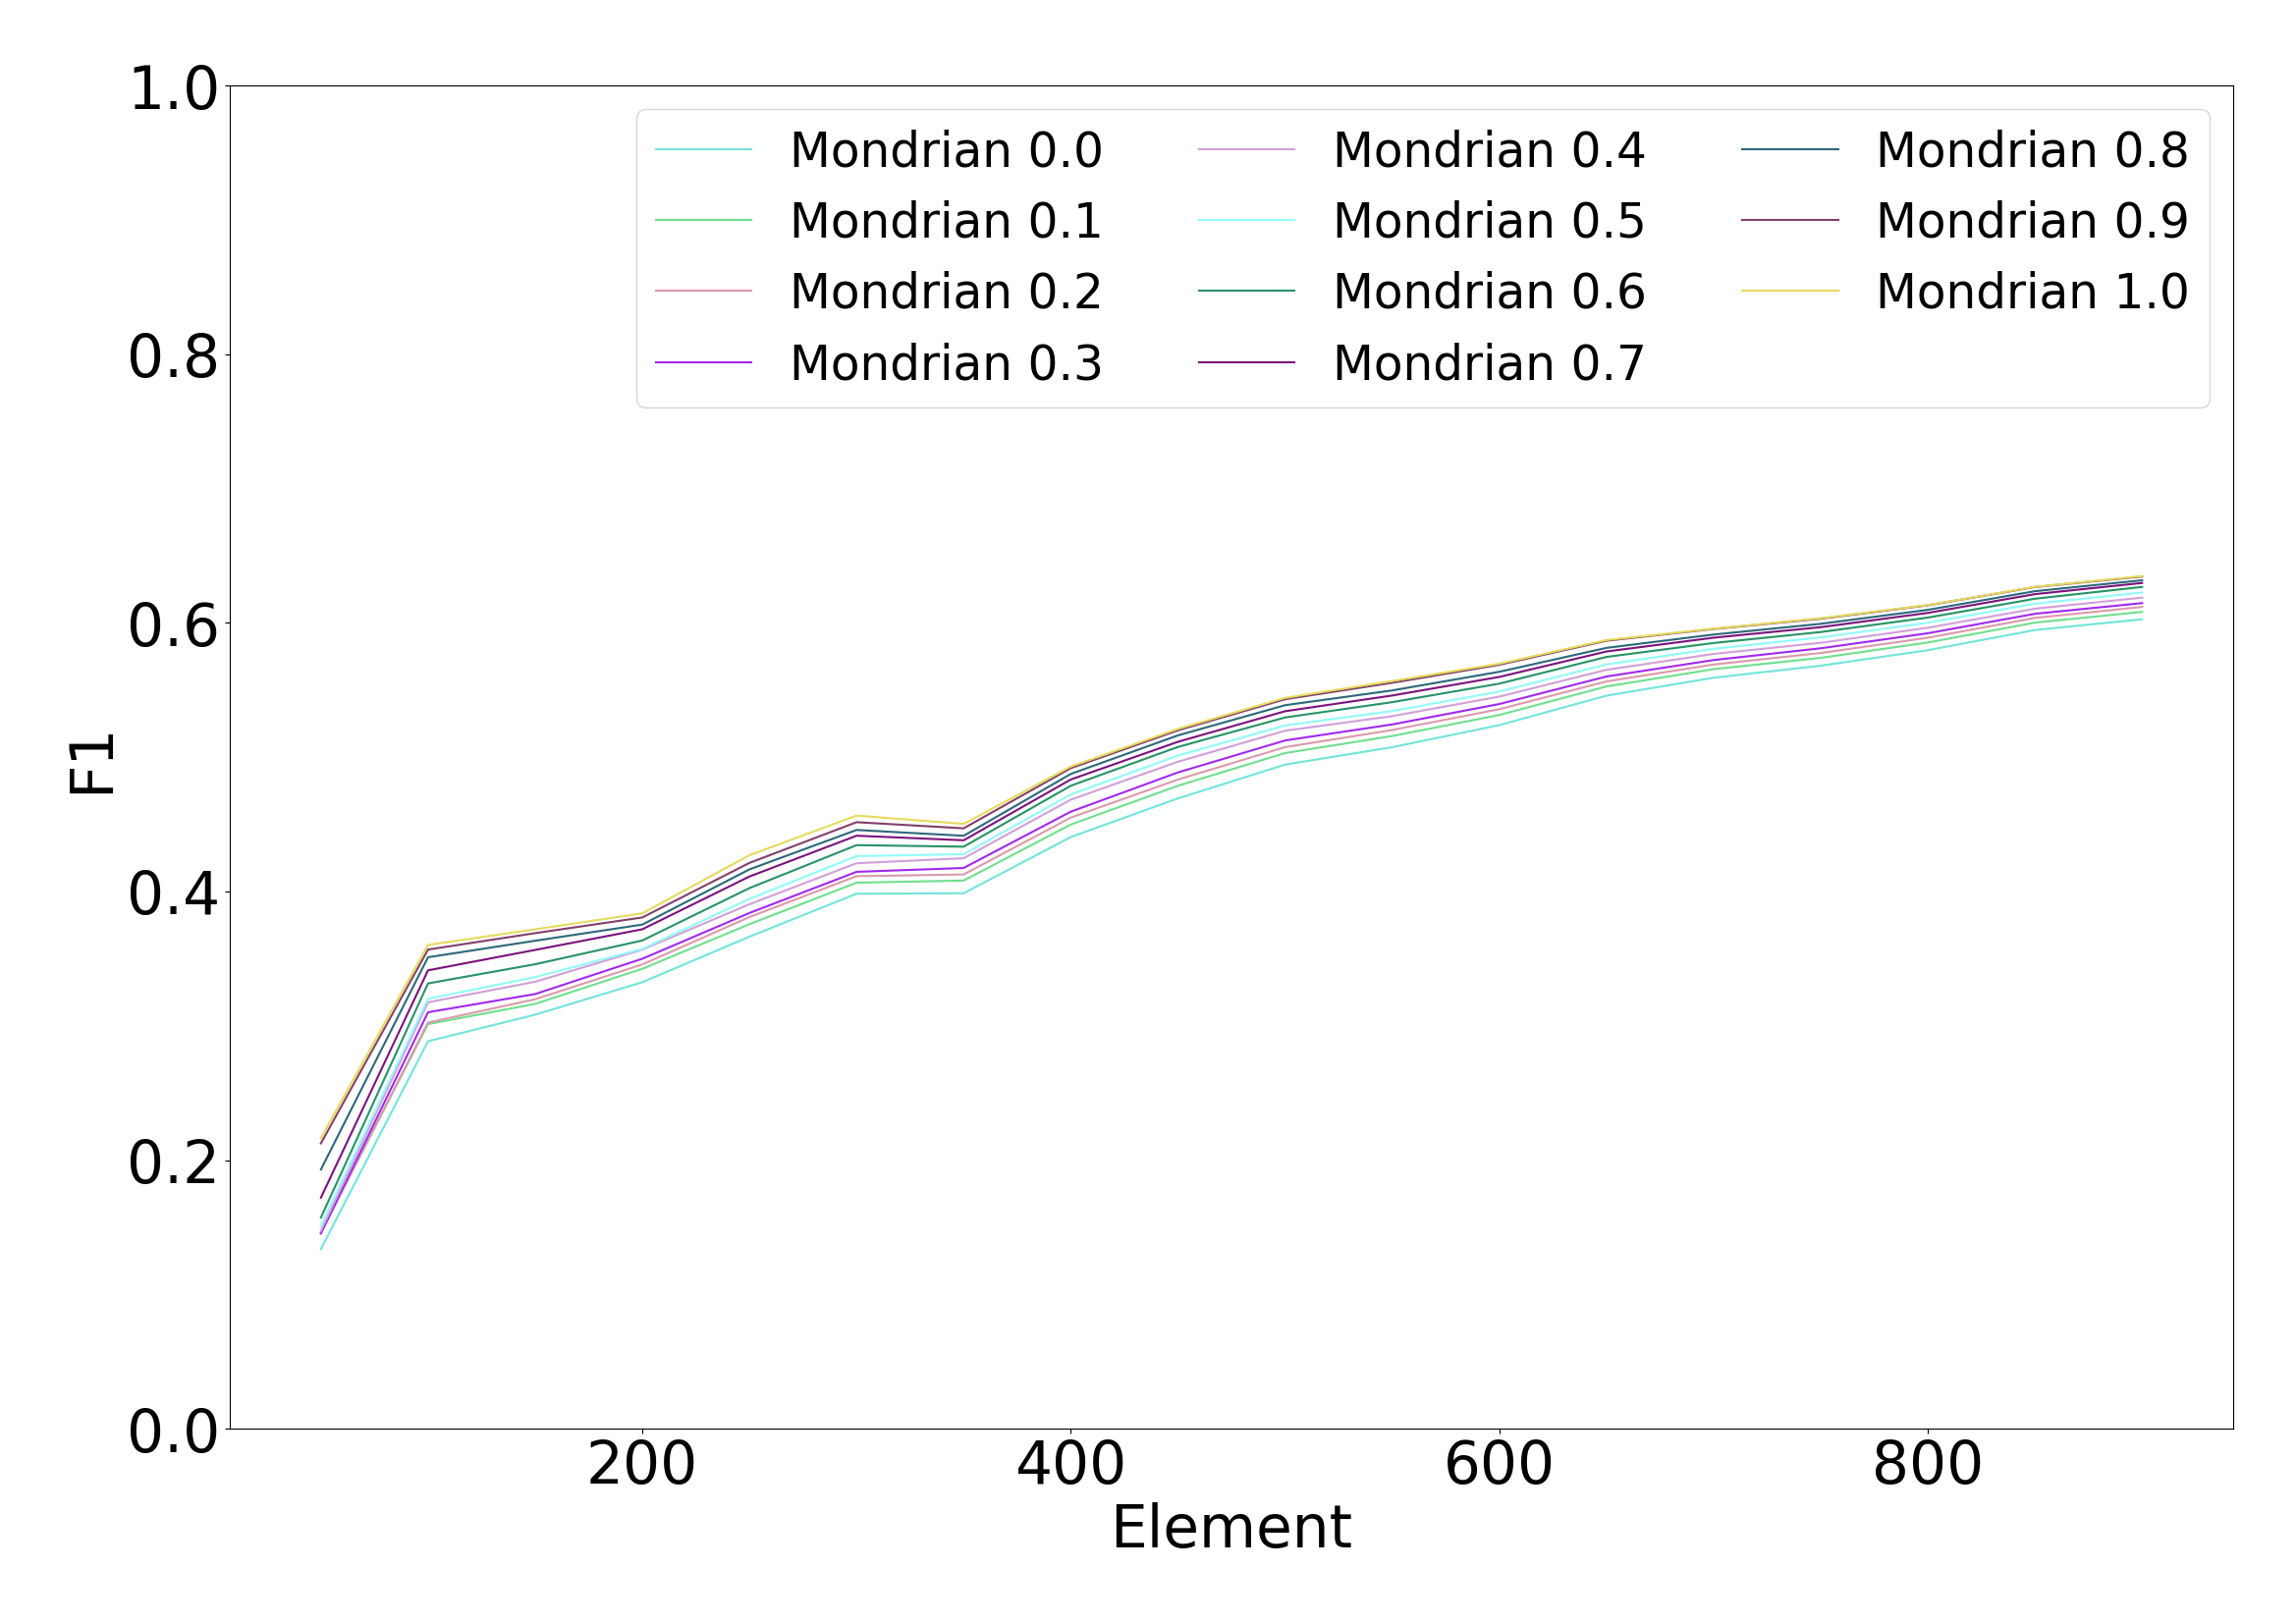
\includegraphics[width=\textwidth]{figures/calibration_mondrian_discount.png}
		 \caption{Impact of the discount factor with 10 trees, a budget of $1.0$, and a base count of $0.1$. \TG{put this graph on the same 0-1 scale as the two other ones.}}
		 \label{fig:mondrian-discount}
	 \end{subfigure}
		\caption{Hyperparameters tuning for Mondrian with first subject of \banosdataset dataset.}
		\label{fig:mondrian-tuning}
\end{figure}


